\documentclass{book}
\usepackage{xcolor}
\usepackage{tikz}

\usepackage{soul}
\usepackage{tikz}
\usetikzlibrary{calc,shapes.multipart,chains,arrows}
\usetikzlibrary{positioning}
\usetikzlibrary{arrows, shapes.gates.logic.US, calc}

\definecolor{darkyellow}{rgb}{0.8, 0.8, 0.0}
\definecolor{lightblue}{rgb}{0.68, 0.85, 0.9}
\definecolor{lightred}{rgb}{1.0, 0.8, 0.8}
\definecolor{lightgreen}{rgb}{0.8, 1.0, 0.8}
\definecolor{lightyellow}{rgb}{1.0, 1.0, 0.8}
\usepackage{colortbl}

\definecolor{forestgreen}{rgb}{0.13, 0.55, 0.13}
\usepackage{amsmath}

\DeclareMathOperator*{\argmax}{arg\,max}
\DeclareMathOperator*{\argmin}{arg\,min}

\usepackage{amsthm}

\usepackage{quantikz}

\usepackage{amssymb}
\newtheorem{definition}{Definition}


\usepackage{tikz-cd}
\usepackage{mdframed}
\usepackage{lipsum}
\usepackage{graphicx}
\graphicspath{ {./images/} }
\usepackage[left=0.5cm,right=0.5cm,top=0.5cm,bottom=0.5cm]{geometry}

\usepackage{circuitikz}
\usepackage{float}
\usepackage{tabularx}
\usepackage{blkarray}% http://ctan.org/pkg/blkarray
\newcommand{\matindex}[1]{\mbox{\scriptsize#1}}% Matrix index

\usepackage{xcolor}
\definecolor{myblue}{rgb}{.8, .8, 1}
\definecolor{mygreen}{rgb}{.8, 1, .8}
\definecolor{myred}{rgb}{1, .8, .8}
\definecolor{myyellow}{rgb}{1, 1, .5}
\definecolor{myorange}{rgb}{1, .8, .5}
\definecolor{mypurple}{rgb}{.8, .5, 1}
\definecolor{mygray}{rgb}{.8, .8, .8}
\definecolor{mycyan}{rgb}{.5, 1, 1}

\usepackage[most]{tcolorbox}
\usepackage{listings}
\usepackage{array}
\usepackage{ulem}

\usepackage{mathtools}
\DeclarePairedDelimiter\ceil{\lceil}{\rceil}
\DeclarePairedDelimiter\floor{\lfloor}{\rfloor}

\setlength\parindent{0pt} % No indent for all paragraphs

\usepackage{wrapfig}
\usepackage{placeins}
\usepackage{venndiagram}
\usepackage{braket}
\usepackage{enumitem}

% Definition Box
\newtcolorbox{defBox}[3][]{
arc=5mm,
lower separated=false,
fonttitle=\bfseries,
colbacktitle=green!10,
coltitle=green!50!black,
enhanced,
attach boxed title to top left={xshift=0.5cm,
        yshift=-2mm},
colframe=green!50!black,
colback=green!10,
overlay={
\node[draw=green!50!black,thick,
%inner sep=2mm,
fill= green!10,rounded corners=1mm, 
yshift=0pt, 
xshift=-0.5cm, 
left, 
text=green!50!black,
anchor=east,
font=\bfseries] 
at (frame.north east) {#3};},
title=#2,#1}

\newtcolorbox{thmBox}[3][]{
arc=5mm,
lower separated=false,
fonttitle=\bfseries,
colbacktitle=blue!10,
coltitle=blue!50!black,
enhanced,
attach boxed title to top left={xshift=0.5cm,     yshift=-2mm},
colframe=blue!50!black,
colback=blue!10,
overlay={
\node[draw=blue!50!black, thick,
fill=blue!10, rounded corners=1mm,
yshift=0pt,
xshift=-0.5cm,
left,
text=blue!50!black,
anchor=east,
font=\bfseries]
at (frame.north east) {#3};},
title=#2,#1}

\newtcolorbox{synBox}[3][]{
arc=5mm,
lower separated=false,
fonttitle=\bfseries,
colbacktitle=yellow!10, % Change green to yellow here
coltitle=yellow!50!black, % Change green to yellow here
enhanced,
attach boxed title to top left={xshift=0.5cm, yshift=-2mm},
colframe=yellow!50!black, % Change green to yellow here
colback=yellow!10, % Change green to yellow here
overlay={
\node[draw=yellow!50!black, thick,
fill=yellow!10, rounded corners=1mm,
yshift=0pt,
xshift=-0.5cm,
left,
text=yellow!50!black,
anchor=east,
font=\bfseries]
at (frame.north east) {#3};},
title=#2,#1}

\newtcolorbox{egBox}[3][]{
arc=5mm,
lower separated=false,
fonttitle=\bfseries,
colbacktitle=red!10,
coltitle=red!50!black,
enhanced,
attach boxed title to top left={xshift=0.5cm, yshift=-2mm},
colframe=red!50!black,
colback=red!10,
overlay={
\node[draw=red!50!black, thick,
fill=red!10, rounded corners=1mm,
yshift=0pt,
xshift=-0.5cm,
left,
text=red!50!black,
anchor=east,
font=\bfseries]
at (frame.north east) {#3};},
    title=#2,#1
}


\usepackage{titlesec}

\setcounter{secnumdepth}{4}

\titleformat{\paragraph}
{\normalfont\normalsize\bfseries}{\theparagraph}{1em}{}
\titlespacing*{\paragraph}
{0pt}{3.25ex plus 1ex minus .2ex}{1.5ex plus .2ex}

\newcommand{\customBox}[1]{%
    \colorbox{yellow}{\fbox{\textcolor{red}{#1}}}%
}

\title{\Large{\textbf{\texttt{\textcolor{teal}{\fbox{\fbox{\textcolor{purple}{PHYS1007: Quantum Information for Everyone}}}}}}}}
\author{
    \texttt{Author: ThunderDora}\\
    \texttt{Instructor: HUANG Shilin}
}
\date{
    \vfill
    \texttt{Last Update: \today}
}

\begin{document}
\maketitle

\tableofcontents
\chapter{Brief History of Computers}
\textcolor{magenta}{\section{\textbf{Computers before ENIAC}}}
\subsection{Chinese Abacus}
\textcolor{cyan}{Chinese Abacus} is a counting tool used since Han Dynasty (2nd century BC).\\
However, there are some limitations:
\begin{itemize}
    \item \textcolor{blue}{Speed and Robustness}: Faster and more reliable than mental computation, but limited by the speed and correctness of the our hand movements.
    \item \textcolor{blue}{Not Automatic}: It requires human intervention to operate.
\end{itemize}
\subsection{Pascaline}
\raggedright
\textcolor{cyan}{Pascaline} is the first mechanical calculator invented by Blaise Pascal in 1642.\\
It can perform addition and subtraction, but it is not automatic with less human errors.\\
\subsection{Difference Engine}
\raggedright
\textcolor{cyan}{Difference Engine} is a \textcolor{purple}{mechanical calculator} designed by \textcolor{purple}{Charles Babbage, the FATHER of the Computer}, in 1822.\\
It can be used to calculate \textcolor{red}{polynomial functions}: \fbox{\textcolor{teal}{$f(x) = a_n x^n + a_{n-1} x^{n-1} + \cdots + a_1 x + a_0$}}.\\
Each column is a "register" that holds a number in decimal form.\\
$\Rightarrow$ Consists of a stack of gears, where each gear corresponds to a digit (0-9).\\
\vspace{0.1cm}
\uline{\textbf{Difference Method}}\\
If the initial value of $x$ is $x_0$, then the value of $f(x)$ can be calculated by:
\begin{align*}
    f(x) &= f(x_0) + (x - x_0) f'(x_0) + \frac{(x - x_0)^2}{2!} f''(x_0) + \cdots + \frac{(x - x_0)^n}{n!} f^{(n)}(x_0)
\end{align*}
\begin{egBox}{Example 1.1}{Computing $f(x)$ using Difference Method}
    \raggedright
    Suppose we want to compute $f(x) = 2x^2 + 3x + 1$ for some integer $x$.\\
    We know $f(0) = 1$, $f(1) = 6$, $f(2) = 15$ and $f(3) = 28$, then we can compute the first differences and second differences.\\
    \textcolor{blue}{First Differences $\triangle f(x)$}:
    \begin{align*}
        & \triangle f(0) = f(1) - f(0) = 6 - 1 = 5\\
        & \triangle f(1) = f(2) - f(1) = 15 - 6 = 9\\
        & \triangle f(2) = f(3) - f(2) = 28 - 15 = 13
    \end{align*}
    \textcolor{blue}{Second Differences $\triangle^2 f(x)$}:\\
    \begin{align*}
        & \triangle^2 f(0) = \triangle f(1) - \triangle f(0) = 9 - 5 = 4\\
        & \triangle^2 f(1) = \triangle f(2) - \triangle f(1) = 13 - 9 = 4 = \triangle^2 f(0)
    \end{align*}
    Since the second differences are the same, we can conclude that the function is a \textcolor{red}{quadratic function}.\\
    Therefore, we can write $f(x) = 2x^2 + 3x + 1$.\\
\end{egBox}
\newpage
\begin{egBox}{Example 1.2}{Computing $f(x)$ using Addition Only}
    \raggedright
    Suppose we want to compute $f(x) = 2x^2 + 3x + 1$ for some integer $x$.\\
    Given $f(0) = 1$, $\triangle f(0) = 5$ and $\triangle^2 f(0) = 4$ as input, we can compute $f(x)$ for arbitrary positive integer $x$ using addition (+) only.\\
    For $f(6)$:
    \begin{center}
        \begin{tabular}{|c|c|c|c|c|c|c|c|}
            \hline
            \rowcolor{lightblue}
            $x$ & 0 & 1 & 2 & 3 & 4 & 5 & 6\\
            \hline
            \cellcolor{lightgreen}{$f(x)$} & 1 & \textcolor{red}{1 + 5 = 6} & \textcolor{red}{6 + 9 = 15} & \textcolor{red}{15 + 13 = 28} & \textcolor{red}{28 + 17 = 45} & \textcolor{red}{45 + 21 = 66} & \textcolor{red}{66 + 25 = 91}\\
            \hline
            \cellcolor{lightgreen}{$\triangle f(x)$} & 5 & \textcolor{blue}{5 + 4 = 9} & \textcolor{blue}{9 + 4 = 13} & \textcolor{blue}{13 + 4 = 17} & \textcolor{blue}{17 + 4 = 21} & \textcolor{blue}{21 + 4 = 25} & \textcolor{blue}{25 + 4 = 29}\\
            \hline
            \cellcolor{lightgreen}{$\triangle^2 f(x)$} & 4 & 4 & 4 & 4 & 4 & 4 & 4\\
            \hline
        \end{tabular}
    \end{center}
    Therefore, we can compute $f(6) = 91$ using addition only.\\
\end{egBox}
\subsection{Analytical Engine}
\raggedright
\textcolor{cyan}{Analytical Engine} is the first \textcolor{purple}{general-purpose computer} designed by Charles Babbage in 1837, which uses punched cards to input data and instructions.\\
However, it was never completed due to the lack of funding.\\
From 1880 to 1910, Babbage's son, Henry Babbage, completed a simplified version of the Analytical Engine called "The Mill" which was able to calculate a list of $\pi, 2\pi, 3\pi, \cdots$ to 29 decimal places.\\
\subsection{Electromechanical Computers}
\raggedright
\textcolor{cyan}{Electromechanical Computers} are computers that use both electrical and mechanical components.\\
\begin{itemize}
    \item \uline{e.g.}: \textcolor{purple}{Engima Machine} used by the Germans during WWII to encrypt and decrypt messages, \textcolor{purple}{Bombes} used by the British to break the Engima code and \textcolor{purple}{Z3} developed by Konrad Zuse in 1941.\\
\end{itemize}
However, there are some limitations for electromechanical computers:
\begin{itemize}
    \item \textcolor{blue}{Low Speed}: Rely on physical movements to operate which limits the speed.
    \item \textcolor{blue}{Unreliable}: Moving parts experience friction and wear out over time (Components would degrade and fail).
\end{itemize}
\subsection{ENIAC}
\raggedright
\textcolor{cyan}{ENIAC (Electronic Numerical Integrator and Computer)} is the first \textcolor{purple}{general-purpose electronic digital computer} designed by John Mauchly and J. Presper Eckert in 1943.\\
It was used to calculate artillery firing tables for the US Army during WWII.\\
\begin{itemize}
    \item \textcolor{blue}{Size}: Weighs 30 tons and occupies 167 square meters.
    \item \textcolor{blue}{Speed}: 5000 additions per second.
    \item \textcolor{blue}{Reliability}: It was reliable and could run for days without errors.
\end{itemize}
\textcolor{magenta}{\section{\textbf{Binary Numbers}}}
Claude Shannon, the father of modern digital circuit design theory, showed that the binary system is the most efficient way to represent numbers in electronic circuits in 1948.\\
\begin{itemize}
    \item \textcolor{blue}{Binary System}: Uses only two digits, 0 and 1, to represent numbers. (Mainly used in computers)
    \item \textcolor{blue}{Decimal System}: Uses ten digits, 0-9, to represent numbers. (Mainly used by humans)
\end{itemize}
\[
\begin{array}{|c|c|c|c|c|c|c|c|c|c|c|}
    \hline
    \text{Decimal} & 0 & 1 & 2 & 3 & 4 & 5 & 6 & 7 & 8 & 9\\
    \hline
    \text{Binary} & 0 & 1 & 10 & 11 & 100 & 101 & 110 & 111 & 1000 & 1001\\
    \hline
\end{array}
\]
\[
\boxed{\textcolor{teal}{A = \sum_k a_k 2^k \quad \text{where} \quad a_k \in \{0, 1\}}}
\]
\begin{egBox}{Example 1.3}{Converting Decimal to Binary}
    \raggedright
    Convert $83$ to binary.\\
    \[
        83 = 64 + 16 + 2 + 1 = 2^6 + 2^4 + 2^1 + 2^0 = \underline{\underline{(1010011)_2}}
    \]
\end{egBox}
\newpage
\begin{egBox}{Example 1.4}{Converting Binary to Decimal}
    \raggedright
    Convert $(1101)_2$ to decimal.\\
    \[
        (1101)_2 = 1 \times 2^3 + 1 \times 2^2 + 0 \times 2^1 + 1 \times 2^0 = \underline{\underline{13}}
    \]
\end{egBox}
\subsection{Binary Fraction}
\raggedright
\textcolor{cyan}{Binary Fraction} is a number that can be expressed as a sum of negative powers of 2.\\
\[
\boxed{\textcolor{teal}{A = \sum_k a_k 2^{-k} \quad \text{where} \quad a_k \in \{0, 1\}}}
\]
\begin{egBox}{Example 1.5}{Converting Decimal to Binary Fraction}
    \raggedright
    \begin{enumerate}
        \item Convert $\frac{1}{2}$ to binary fraction.\\
        \[
            \frac{1}{2} = 2^{-1} = \underline{\underline{(0.1)_2}}
        \]
        \item Convert $\frac{1}{3}$ to binary fraction.\\
        \[
            \frac{1}{3} = \frac{1}{4} + \frac{1}{8} + \frac{1}{16} + \cdots = \underline{\underline{(0.0101\cdots)_2}}
        \]
    \end{enumerate}
\end{egBox}
\subsection{Binary Addition}
\raggedright
\begin{wrapfigure}[4]{r}{0.3\textwidth}
    \[
    \begin{array}{c@{}c@{}c@{}c@{}c@{}c@{}c@{}c}
        & \textcolor{olive}{1} & \textcolor{olive}{1} & \textcolor{olive}{1} & \textcolor{olive}{1} & \textcolor{olive}{1} & & \hspace{3mm} \textcolor{olive}{\text{Carry Bits}}\\
        &  & 0 & 1 & 1 & 0 & 1 & = \textcolor{blue}{(13)_{10}}\\
        + &  & 1 & 0 & 1 & 1 & 1 & = \textcolor{blue}{(23)_{10}}\\
        \hline
        & 1 & 0 & 0 & 1 & 0 & 0 & = \textcolor{blue}{(36)_{10}}
    \end{array}
    \]
\end{wrapfigure}
\textcolor{cyan}{Binary Addition} is the process of adding two binary numbers.\\
\begin{itemize}
    \item \(0 + 0 = 0\)
    \item \(0 + 1 = 1 + 0 = 1\)
    \item \(1 + 1 = 10\) (Carry 1 to the next column)
\end{itemize}
\subsection{Binary Subtraction}
\raggedright
\begin{wrapfigure}[4]{r}{0.3\textwidth}
    \[
    \begin{array}{c@{}c@{}c@{}c@{}c@{}c@{}c@{}c@{}c}
        & & * & & * & * & * & & \hspace{3mm} \textcolor{olive}{\text{Borrow Bits}}\\
        & 1 & 1 & 0 & 1 & 1 & 1 & 0 & = \textcolor{blue}{(110)_{10}}\\
        - & & & 1 & 0 & 1 & 1 & 1 & = \textcolor{blue}{(23)_{10}}\\
        \hline
        & 1 & 0 & 1 & 0 & 1 & 1 & 1 & = \textcolor{blue}{(87)_{10}}
    \end{array}
    \]
\end{wrapfigure}
\textcolor{cyan}{Binary Subtraction} is the process of subtracting two binary numbers.\\
\begin{itemize}
    \item \(0 - 0 = 1 - 1 = 0\)
    \item \(1 - 0 = 1\)
    \item \(0 - 1 = 1\) (Borrow 1 from the next column)
\end{itemize}
\subsection{Binary Multiplication}
\raggedright
\begin{wrapfigure}[3]{r}{0.3\textwidth}
    \[
    \begin{array}{c@{}c@{}c@{}c@{}c@{}c@{}c@{}c@{}c}
        & & & & 1 & 0 & 1 & 1 & = \textcolor{blue}{(11)_{10}}\\
        \times & & & & 1 & 0 & 1 & 0 & = \textcolor{blue}{(10)_{10}}\\
        \hline
        & & & & 0 & 0 & 0 & 0 & \\
        + & & & 1 & 0 & 1 & 1 & & \\
        + & & 0 & 0 & 0 & 0 & & & \\
        + & 1 & 0 & 1 & 1 & & & & \\
        \hline
        & 1 & 1 & 0 & 1 & 1 & 1 & 0 & 
        \hspace{3mm} = \textcolor{blue}{(110)_{10}}
    \end{array}
    \]
\end{wrapfigure}
\textcolor{cyan}{Binary Multiplication} is the process of multiplying two binary numbers.\\
\begin{itemize}
    \item \(0 \times 0 = 0 \times 1 = 1 \times 0 = 0\)
    \item \(1 \times 1 = 1\)
\end{itemize}
\vspace{0.5cm}
\subsection{Binary Division}
\raggedright
\begin{wrapfigure}[4]{r}{0.2\textwidth}
    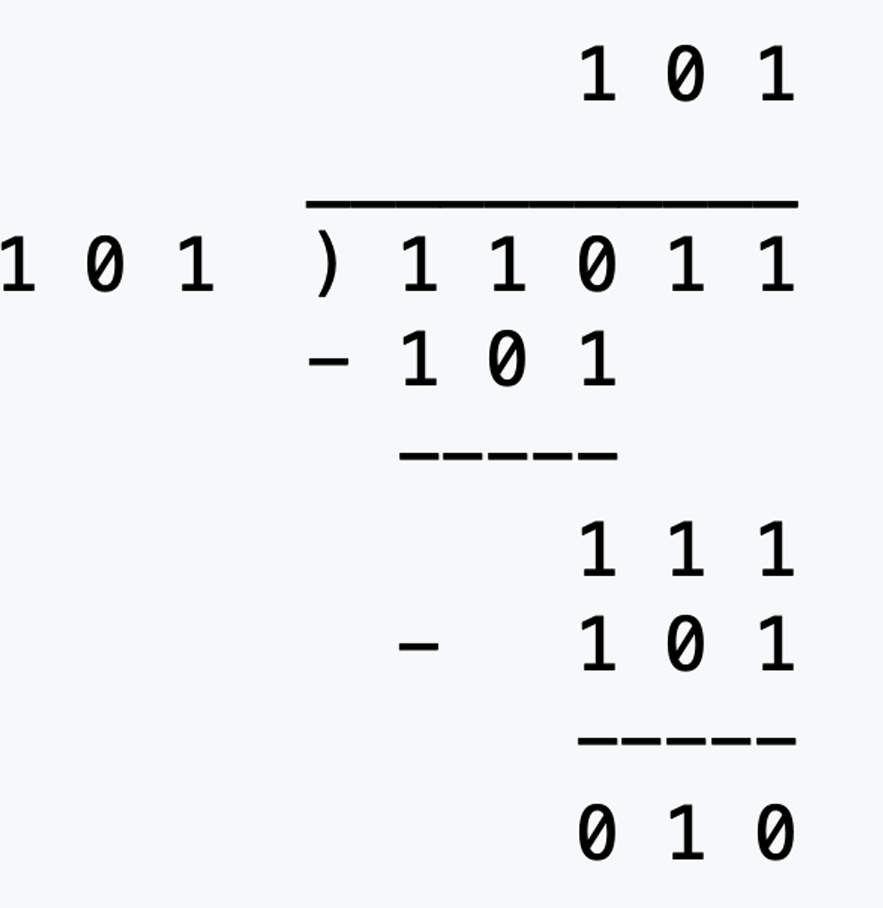
\includegraphics[scale=0.12]{ch1/ch1_figure1.jpeg}
\end{wrapfigure}
\textcolor{cyan}{Binary Division} is the process of dividing two binary numbers.\\
\begin{itemize}
    \item \(0 \div 1 = 0\)
    \item \(1 \div 1 = 1\)
    \item \(1 \div 0 = 0 \div 0 = \text{Undefined}\)
\end{itemize}
\newpage
\textcolor{magenta}{\section{\textbf{Base-$b$ Representation and Horner's Method}}}
We use $(a_{n-1}a_{n-2}\cdots a_1a_0)_b$ to represent a $n$-digit number in base $b$ where $b > 1$.\\
$\implies$ The value of the number is:
\[
\boxed{\textcolor{teal}{A = \sum_{k=0}^{n-1} a_k b^k}} \quad \text{where} \quad a_k \in \{0, 1, \cdots, b-1\}
\]
\begin{egBox}{Example 1.6}{Representing a Number in Different Bases}
    \raggedright
    Represent $13$ in base $10$, base $8$ and base $16$.\\
    \begin{itemize}
        \item Base $10$: $13 = 1 \times 10^1 + 3 \times 10^0 = \underline{\underline{(13)_{10}}}$
        \item Base $8$: $13 = 1 \times 8^1 + 5 \times 8^0 = \underline{\underline{(15)_8}}$
        \item Base $16$: $13 = 0 \times 16^1 + 13 \times 16^0 = \underline{\underline{(D)_{16}}}$
    \end{itemize}
\end{egBox}
\fbox{
    \parbox{0.97\textwidth}{
        \textit{\textbf{Remark}}: For hexadecimal numbers (base-16), we use the digits 0-9 and the letters A-F to represent the numbers 10-15.
    }
}\\
\vspace{0.3cm}
\uline{\textbf{\large Horner's Method}}\\
\begin{thmBox}{Theorem 1.1}{Horner's Method}
    \raggedright
    \textcolor{cyan}{Horner's Method} is a method to convert a number from base $b$ to base $10$.\\
    For Integers:
    \[
    \boxed{\textcolor{teal}{\sum_{k=0}^{n-1} a_k b^{k-1} = a_0 + b(a_1 + b(a_2 + b(a_3 + \cdots + b(a_{n-1})\cdots)))}}
    \]
    For Fractions:
    \[
    \boxed{\textcolor{teal}{\sum_{k=1}^{n} a_{-k} b^{-k} = a_{-1} + b(a_{-2} + b(a_{-3} + \cdots + b(a_{-n})\cdots))}}
    \]
\end{thmBox}
\begin{egBox}{Example 1.7}{Converting a Decimal Number to Binary using Horner's Method}
    \raggedright
    Convert $(35)_{10}$ to binary.\\
    \[
    \begin{array}{rcl}
        35 &=& 2 \times 17 \colorbox{yellow}{+1} \\
        17 &=& 2 \times 8 \colorbox{yellow}{+1} \\
        8 &=& 2 \times 4 \colorbox{yellow}{+0} \\
        4 &=& 2 \times 2 \colorbox{yellow}{+0} \\
        2 &=& 2 \times 1 \colorbox{yellow}{+0} \\
        1 &=& 2 \times 0 \colorbox{yellow}{+1} \\
    \end{array}
    \]
    $\therefore$ $(35)_{10} = \underline{\underline{(100011)_2}}$
\end{egBox}
\begin{egBox}{Example 1.8}{Converting a Decimal Fraction to Binary using Horner's Method}
    \raggedright
    Convert $\frac{1}{3}$ to binary.\\
    \[
    \begin{array}{rcl}
        & & \frac{1}{3} < 1 \implies \text{Real Number} = 0. \\
        \vspace{0.1cm}
        \frac{1}{3} \times 2 &=& \frac{2}{3} < 1 \implies \text{Real Number} = 0.0 \\
        \vspace{0.1cm}
        \frac{2}{3} \times 2 &=& \frac{4}{3} > 1 \implies \text{Real Number} = 0.01 \\
        \vspace{0.1cm}
        \frac{1}{3} \times 2 &=& \frac{2}{3} < 1 \implies \text{Real Number} = 0.010 \\
        \vspace{0.1cm}
        \frac{2}{3} \times 2 &=& \frac{4}{3} > 1 \implies \text{Real Number} = 0.0101 \\
        \vspace{0.1cm}
        \ldots & & \\
    \end{array}
    \]
    $\therefore$ $\frac{1}{3} = \underline{\underline{(0.0101\cdots)_2}}$
\end{egBox}


\newpage
\textcolor{magenta}{\section{\textbf{Boolean Algebra}}}
\textcolor{cyan}{Boolean Algebra} is a branch of algebra introduced by George Boole  that deals with variables that can take on one of two values, \textcolor{purple}{0 or 1 (True or False)}.\\
\uline{\textbf{Three Basic Operations}}:
\vspace{0.2cm}
\begin{itemize}
    \item \textcolor{blue}{Conjunction (AND)}: \fbox{\textcolor{teal}{\(x \land y = x \cdot y\)}}\\
    If \(x = 1\) and \(y = 1\), then \(x \land y = 1\). Otherwise, \(x \land y = 0\).
    \begin{center}
        \begin{venndiagram2sets}[labelA=$x$, labelB=$y$, radius=1.15cm]
            \setkeys{venn}{shade = red}
            \fillACapB
        \end{venndiagram2sets}
    \end{center}
    \item \textcolor{blue}{Disjunction (OR)}: \fbox{\textcolor{teal}{\(x \lor y = x + y\)}}\\
    If \(x = 0\) and \(y = 0\), then \(x \lor y = 0\). Otherwise, \(x \lor y = 1\).
    \begin{center}
        \begin{venndiagram2sets}[labelA=$x$, labelB=$y$, radius=1.15cm]
            \setkeys{venn}{shade = red}
            \fillA \fillB
        \end{venndiagram2sets}
    \end{center}
    \item \textcolor{blue}{Negation (NOT)}: \fbox{\textcolor{teal}{\(\neg x = 1 - x\)}} or \fbox{\textcolor{teal}{\(\overline{x}\)}}\\
    If \(x = 1\), then \(\neg x = 0\). Otherwise, \(\neg x = 1\).
    \begin{center}
        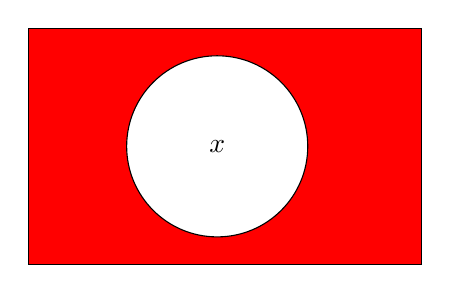
\begin{tikzpicture}
            
            \fill[red] (-1.5,-1.5) rectangle (3.5,1.5);
            \draw[fill=white] (0.9,0) circle (1.15cm);
            \draw (-1.5,-1.5) rectangle (3.5,1.5);
            \node at (0.9,0) {\(x\)};
        \end{tikzpicture}
    \end{center}
\end{itemize}
\textcolor{cyan}{Truth Table} is a table that shows the output of a Boolean function for all possible input values.\\
Here are the truth tables for the basic operations:
\begin{center}
    \begin{tabular}{|c|c|c|c|c|}
        \hline
        \rowcolor{lightblue}
        \(x\) & \(y\) & \(x \land y\) & \(x \lor y\) & \(\neg x\)\\
        \hline
        0 & 0 & 0 & 0 & 1\\
        0 & 1 & 0 & 1 & 1\\
        1 & 0 & 0 & 1 & 0\\
        1 & 1 & 1 & 1 & 0\\
        \hline
    \end{tabular}
\end{center}

\uline{\textbf{Other Basic Operations Built from the Three Basic Operations}}:
\begin{wrapfigure}[4]{r}{0.3\textwidth}
    \begin{tabular}{|c|c|c|c|c|}
        \hline
        \rowcolor{lightblue}
        \(x\) & \(y\) & \(x \rightarrow y\) & \(x \oplus y\) & \(x \leftrightarrow y\)\\
        \hline
        0 & 0 & 1 & 0 & 1\\
        0 & 1 & 1 & 1 & 0\\
        1 & 0 & 0 & 1 & 0\\
        1 & 1 & 1 & 0 & 1\\
        \hline
    \end{tabular}
\end{wrapfigure}
\begin{itemize}
    \item \textcolor{blue}{Implication (IMPL)}: \fbox{\textcolor{teal}{\(x \rightarrow y = \neg x \lor y\)}}\\
    \item \textcolor{blue}{Exclusive OR (XOR)}: \fbox{\textcolor{teal}{\(x \oplus y = (x \land \neg y) \lor (\neg x \land y)\)}}\\
    \item \textcolor{blue}{Equality (EQ)}: \fbox{\textcolor{teal}{\(x \leftrightarrow y = (x \land y) \lor (\neg x \land \neg y)\)}}\\
    \item \textcolor{blue}{De Morgan's Laws}: \fbox{\textcolor{teal}{\(x \land y = \neg (\neg x \lor \neg y)\)}} and \fbox{\textcolor{teal}{\(x \lor y = \neg (\neg x \land \neg y)\)}}\\
\end{itemize}
\newpage
\textcolor{magenta}{\section{\textbf{Boolean Functions}}}
\begin{defBox}{Definition 1.1}{Boolean Function}
    \raggedright
    A \textcolor{cyan}{Boolean Function} is a function that takes input values from a set of Boolean variables and returns a single Boolean value.\\
    \[
    \boxed{\textcolor{teal}{f: \{0, 1\}^k \rightarrow \{0, 1\}}}
    \]
\end{defBox}
\begin{egBox}{Example 1.9}{Boolean Function of AND Gate}
    For an AND Gate with $k=2$ inputs and $m=1$ output, the Boolean function is:
    \[
    \begin{array}{|c|c|c|}
        \hline
        \rowcolor{lightblue}
        $$x_1$$ & $$x_2$$ & $$f(x_1, x_2)$$\\
        \hline
        0 & 0 & 0\\
        0 & 1 & 0\\
        1 & 0 & 0\\
        1 & 1 & 1\\
        \hline
    \end{array}
    \]
    Therefore, the Boolean function of an AND Gate is:
    \[
    \boxed{\textcolor{teal}{f(x_1, x_2) = x_1 \land x_2}}
    \]
\end{egBox}
\begin{egBox}{Example 1.10}{Boolean Function of Parity Function}
    \fbox{\textcolor{cyan}{Parity Function} is a function that \textcolor{red}{returns 1 if the number of 1's in the input is odd, and 0 otherwise}}.\\
    \vspace{0.2cm}
    For a Parity Function with $k=3$ inputs and $m=1$ output, the Boolean function is:
    \[
    \begin{array}{|c|c|c|c|}
        \hline
        \rowcolor{lightblue}
        $$x_0$$ & $$x_1$$ & $$x_2$$ & $$f(x_0, x_1, x_2)$$\\
        \hline
        0 & 0 & 0 & 0\\
        0 & 0 & 1 & 1\\
        0 & 1 & 0 & 1\\
        0 & 1 & 1 & 0\\
        1 & 0 & 0 & 1\\
        1 & 0 & 1 & 0\\
        1 & 1 & 0 & 0\\
        1 & 1 & 1 & 1\\
        \hline
    \end{array}
    \]
    Therefore, the Boolean function of a Parity Function is:
    \[
    \boxed{\textcolor{teal}{f(x_0, x_1, x_2) = x_0 \oplus x_1 \oplus x_2}}
    \]
\end{egBox}
In Boolean Function, there are two types of adders:
\begin{enumerate}
    \item \textcolor{cyan}{Half Adder}: Adds two bits and produces a sum and a carry bit.
    \[
        \boxed{\textcolor{teal}{f(a,b) = (c, s) = (a \land b, a \oplus b)}} \quad \text{where} \quad a, b \in \{0, 1\}
    \]
    \begin{itemize}
        \item \textcolor{blue}{Sum Bit}: \(s = a \oplus b\)
        \item \textcolor{blue}{Carry Bit}: \(c = a \land b\)
    \end{itemize}
    \item \textcolor{cyan}{Full Adder}: Adds three bits and produces a sum and a carry bit.
    \[
        \boxed{\textcolor{teal}{f(a,b,c_{in}) = (c_{out}, s) = ((a \land b) \lor (b \land c_{in}) \lor (a \land c_{in}), a \oplus b \oplus c_{in})}} \quad \text{where} \quad a, b, c_{in} \in \{0, 1\}
    \]
    \begin{itemize}
        \item \textcolor{blue}{Sum Bit}: \(s = a \oplus b \oplus c_{in}\)
        \item \textcolor{blue}{Carry-in Bit generated by the Addition of Lower-order Bits}: \(c_{in} = a \land b\)
        \item \textcolor{blue}{Carry-out Bit passed to the Next Higher-order Bit}: \(c_{out} = (a \land b) \lor (b \land c_{in}) \lor (a \land c_{in})\)
    \end{itemize}
\end{enumerate}
\newpage
\textcolor{magenta}{\section{\textbf{Logic Circuits}}}
\subsection{Logic Gates}
There are 7 types of logic gates in Boolean Algebra:
\begin{enumerate}
    \item \textcolor{cyan}{AND Gate}: Outputs 1 if all inputs are 1.
    \[
        \boxed{\textcolor{teal}{\text{AND}(a, b) = a \land b}}
    \]
    \begin{center}
        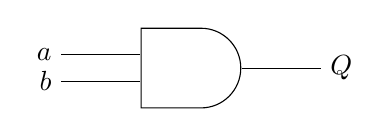
\begin{tikzpicture}
            \node[and gate US, draw, rotate=0, logic gate inputs=nn, scale=2] at (0,0) (and1) {};
            \draw (and1.input 1) -- ++(-1,0) node[left] {\(a\)};
            \draw (and1.input 2) -- ++(-1,0) node[left] {\(b\)};
            \draw (and1.output) -- ++(1,0) node[right] {\(Q\)};
        \end{tikzpicture}
    \end{center}
    \item \textcolor{cyan}{OR Gate}: Outputs 1 if at least one input is 1.
    \[
        \boxed{\textcolor{teal}{\text{OR}(a, b) = a \lor b}}
    \]
    \begin{center}
        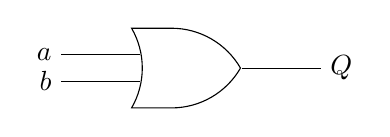
\begin{tikzpicture}
            \node[or gate US, draw, rotate=0, logic gate inputs=nn, scale=2] at (0,0) (or1) {};
            \draw (or1.input 1) -- ++(-1,0) node[left] {\(a\)};
            \draw (or1.input 2) -- ++(-1,0) node[left] {\(b\)};
            \draw (or1.output) -- ++(1,0) node[right] {\(Q\)};
        \end{tikzpicture}
    \end{center}
    \item \textcolor{cyan}{NOT Gate}: Outputs 1 if the input is 0.
    \[
        \boxed{\textcolor{teal}{\text{NOT}(a) = \neg a}}
    \]
    \begin{center}
        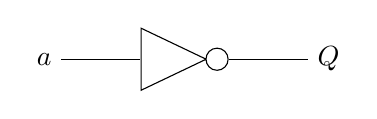
\begin{tikzpicture}
            \node[not gate US, draw, rotate=0, scale=2] at (0,0) (not1) {};
            \draw (not1.input) -- ++(-1,0) node[left] {\(a\)};
            \draw (not1.output) -- ++(1,0) node[right] {\(Q\)};
        \end{tikzpicture}
    \end{center}
    \item \textcolor{cyan}{NAND Gate}: Outputs 0 if all inputs are 1.
    \[
        \boxed{\textcolor{teal}{\text{NAND}(a, b) = \text{NOT}(\text{AND}(a, b)) = \neg (a \land b)}}
    \]
    \begin{center}
        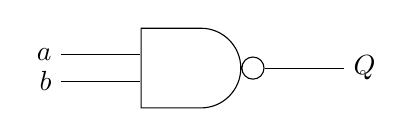
\begin{tikzpicture}
            \node[nand gate US, draw, rotate=0, logic gate inputs=nn, scale=2] at (0,0) (nand1) {};
            \draw (nand1.input 1) -- ++(-1,0) node[left] {\(a\)};
            \draw (nand1.input 2) -- ++(-1,0) node[left] {\(b\)};
            \draw (nand1.output) -- ++(1,0) node[right] {\(Q\)};
        \end{tikzpicture}
    \end{center}
    \item \textcolor{cyan}{NOR Gate}: Outputs 0 if at least one input is 1.
    \[
        \boxed{\textcolor{teal}{\text{NOR}(a, b) = \text{NOT}(\text{OR}(a, b)) = \neg (a \lor b)}}
    \]
    \begin{center}
        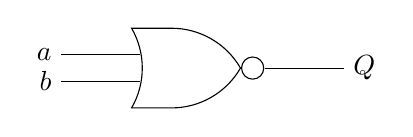
\begin{tikzpicture}
            \node[nor gate US, draw, rotate=0, logic gate inputs=nn, scale=2] at (0,0) (nor1) {};
            \draw (nor1.input 1) -- ++(-1,0) node[left] {\(a\)};
            \draw (nor1.input 2) -- ++(-1,0) node[left] {\(b\)};
            \draw (nor1.output) -- ++(1,0) node[right] {\(Q\)};
        \end{tikzpicture}
    \end{center}
    \item \textcolor{cyan}{XOR Gate}: Outputs 1 if the number of 1's in the input is odd.
    \[
        \boxed{\textcolor{teal}{\text{XOR}(a, b) = a \oplus b}}
    \]
    \begin{center}
        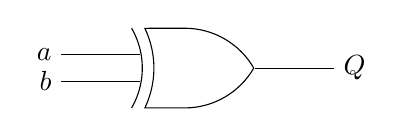
\begin{tikzpicture}
            \node[xor gate US, draw, rotate=0, logic gate inputs=nn, scale=2] at (0,0) (xor1) {};
            \draw (xor1.input 1) -- ++(-1,0) node[left] {\(a\)};
            \draw (xor1.input 2) -- ++(-1,0) node[left] {\(b\)};
            \draw (xor1.output) -- ++(1,0) node[right] {\(Q\)};
        \end{tikzpicture}
    \end{center}
    \item \textcolor{cyan}{XNOR Gate}: Outputs 1 if the number of 1's in the input is even.
    \[
        \boxed{\textcolor{teal}{\text{XNOR}(a, b) = \text{NOT}(\text{XOR}(a, b)) = \text{EQUAL}(a, b) = \neg (a \oplus b)}}
    \]
    \begin{center}
        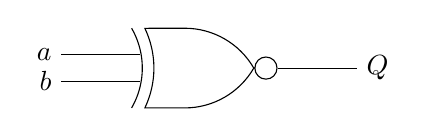
\begin{tikzpicture}
            \node[xnor gate US, draw, rotate=0, logic gate inputs=nn, scale=2] at (0,0) (xnor1) {};
            \draw (xnor1.input 1) -- ++(-1,0) node[left] {\(a\)};
            \draw (xnor1.input 2) -- ++(-1,0) node[left] {\(b\)};
            \draw (xnor1.output) -- ++(1,0) node[right] {\(Q\)};
        \end{tikzpicture}
    \end{center}
\end{enumerate}
\newpage
The truth tables for the logic gates are as follows:
\begin{center}
    \begin{tabular}{|c|c|c|c|c|c|c|c|c|}
        \hline
        \rowcolor{lightblue}
        \(a\) & \(b\) & \(\text{AND}(a, b)\) & \(\text{OR}(a, b)\) & \(\text{NOT}(a)\) & \(\text{NAND}(a, b)\) & \(\text{NOR}(a, b)\) & \(\text{XOR}(a, b)\) & \(\text{XNOR}(a, b)\)\\
        \hline
        0 & 0 & 0 & 0 & 1 & 1 & 1 & 0 & 1\\
        0 & 1 & 0 & 1 & 1 & 1 & 0 & 1 & 0\\
        1 & 0 & 0 & 1 & 0 & 1 & 0 & 1 & 0\\
        1 & 1 & 1 & 1 & 0 & 0 & 0 & 0 & 1\\
        \hline
    \end{tabular}
\end{center}
\subsection{Logic Circuits: Half Adder and Full Adder}
\uline{\textbf{Half Adder}}:\\
The boolean function of a half adder is:
\begin{align*}
    & \boxed{\textcolor{teal}{\text{Half Adder}(A, B) = (C, S) = (A \land B, A \oplus B)}} \quad \text{where} \quad A, B \in \{0, 1\} \\
    & \text{Carry Bit: } C = A \land B\\
    & \text{Sum Bit: } S = A \oplus B
\end{align*}
\begin{center}
    \begin{circuitikz}
        \draw
        (0,0) node[label = left: A] (sam) {} -- (3, 0)
        node [xor port, anchor=in 1] (xor1) {XOR} 
        (0, 52 |- xor1.in 2) node[label = left: B] (sam) {} -- (3, 52 |- xor1.in 2)
        (xor1.out) -- ++(1,0) node[label = right: S] {}
        (3, -2) node [and port, anchor=in 1] (and1) {AND}
        (and1.in 1) -- ++(-1,0) to [short, -*] (2, 0)
        (and1.in 2) -- ++(-2,0) to [short, -*] (1, 52 |- xor1.in 2)
        (and1.out) -- ++(1,0) node[label = right: C] {};
    \end{circuitikz}
\end{center}
The truth table for a half adder is:
\begin{center}
    \begin{tabular}{|c|c|c|c|}
        \hline
        \rowcolor{lightblue}
        \(A\) & \(B\) & \(S\) & \(C\)\\
        \hline
        0 & 0 & 0 & 0\\
        0 & 1 & 1 & 0\\
        1 & 0 & 1 & 0\\
        1 & 1 & 0 & 1\\
        \hline
    \end{tabular}
\end{center}
Half Adder is used to \textcolor{purple}{add two bits and produce a sum and a carry bit}, we can illustrate the half adder as follows:
\begin{center}
    \[
        \begin{array}{c@{}c@{}c@{}c@{}c@{}c@{}c@{}c}
            & \textcolor{olive}{1} & \textcolor{olive}{1} & \textcolor{olive}{1} & \textcolor{olive}{1} & \textcolor{olive}{1}^{\textcolor{red}{C}} & & \hspace{3mm} \textcolor{olive}{\text{Carry Bits}}\\
            &  & 0 & 1 & 1 & 0 & 1^{\textcolor{red}{A}} & = \textcolor{blue}{(13)_{10}}\\
            + &  & 1 & 0 & 1 & 1 & 1^{\textcolor{red}{B}} & = \textcolor{blue}{(23)_{10}}\\
            \hline
            & 1 & 0 & 0 & 1 & 0 & 0^{\textcolor{red}{S}} & = \textcolor{blue}{(36)_{10}}
        \end{array}
    \]
\end{center}
\uline{\textbf{Full Adder}}:\\
The boolean function of a full adder is:
\begin{align*}
    & \boxed{\textcolor{teal}{\text{Full Adder}(A, B, C_{in}) = (C_{out}, S) = ((A \land B) \lor (B \land C_{in}) \lor (A \land C_{in}), A \oplus B \oplus C_{in})}} \quad \text{where} \quad A, B, C_{in} \in \{0, 1\} \\
    & \text{Carry-out Bit: } C_{out} = (A \land B) \lor (B \land C_{in}) \lor (A \land C_{in})\\
    & \text{Sum Bit: } S = A \oplus B \oplus C_{in}
\end{align*}
\begin{center}
    \begin{circuitikz}
        \draw (0,8) node[xor port](xor1){XOR}
        (-4.25, 8.25) node[anchor=east] {A} %%input A
        (-4.25, 7.75) node[anchor=east] {B} %%input B
        (-4, 6.75) node[anchor=east] {$\text{C}_{in}$} %%input C_in
        (2, 7.5) node[xor port] (xor2){XOR} 
        (xor2.out) node[anchor=west] {S}
        (2, 5.5) node[and port] (and1){AND}
        (2, 3.5) node[and port] (and2){AND}
        (4, 4.5) node[or port] (or){OR}
        (-4, 8.28) to[short, -*](-3, 8.28)-|(xor1.in 1)
        (-4, 7.72) to[short, -*](-2.5, 7.72)-|(xor1.in 2)
        (-4, 6.75) to[short, -*](0.6, 6.75)-|(and1.in 1)
        (0, 6.75)-|(xor2.in 2)
        (0, 8) to[short, -*](0.25, 8)-|(xor2.in 1)

        (0.25, 8)--(0.25, 5.22)-|(and1.in 2)
        (-3, 8.28)--(-3, 3.22)-|(and2.in 2)
        (-2.5, 7.72)--(-2.5, 3.78)-|(and2.in 1)
        (and1.out)-|(or.in 1)
        (and2.out)-|(or.in 2)
        (or.out) node[anchor=west]{$\text{C}_{out}$}
        ;
    \end{circuitikz}
\end{center}
\newpage
The truth table for a full adder is:
\begin{center}
    \begin{tabular}{|c|c|c|c|c|c|c|}
        \hline
        \rowcolor{lightblue}
        \(A\) & \(B\) & \(C_{in}\) & \(S\) & \(C_{out}\)\\
        \hline
        0 & 0 & 0 & 0 & 0\\
        0 & 0 & 1 & 1 & 0\\
        0 & 1 & 0 & 1 & 0\\
        0 & 1 & 1 & 0 & 1\\
        1 & 0 & 0 & 1 & 0\\
        1 & 0 & 1 & 0 & 1\\
        1 & 1 & 0 & 0 & 1\\
        1 & 1 & 1 & 1 & 1\\
        \hline
    \end{tabular}
\end{center}
Full Adder is used to \textcolor{purple}{add three bits and produce a sum and a carry-out bit}.
\begin{itemize}
    \item Check $S$: \textcolor{forestgreen}{If there are an odd number of 1's among the three bits, then $S = 1$. Otherwise, $S = 0$.}
    \item Check $C_{out}$:
    \begin{itemize}
        \item \textcolor{blue}{Case 1}: \textcolor{forestgreen}{If $A \land B = 1$}, then \textcolor{orange}{$C_{out} = 1$}.
        \item \textcolor{blue}{Case 2}: \textcolor{forestgreen}{If $A \oplus B = 1$ and $C_{in} = 1$}, then \textcolor{orange}{$C_{out} = 1$}.
        \item \textcolor{blue}{Case 3}: \textcolor{forestgreen}{If $A = 0$ and $B = 0$}, then \textcolor{orange}{$C_{out} = 0$}.
    \end{itemize}
\end{itemize}
We can illustrate the full adder as follows:
\begin{center}
    \[
        \begin{array}{c@{}c@{}c@{}c@{}c@{}c@{}c@{}c}
            & & & \textcolor{red}{\text{\small C}_{\text{out}}} & \textcolor{red}{\text{\small C}_{\text{in}}} & & & \\
            & \textcolor{olive}{1} & \textcolor{olive}{1} & \textcolor{olive}{1} & \textcolor{olive}{1} & \textcolor{olive}{1} & & \hspace{3mm} \textcolor{olive}{\text{Carry Bits}}\\
            &  & 0 & 1 & 1^{\textcolor{red}{A}} & 0 & 1 & = \textcolor{blue}{(13)_{10}}\\
            + &  & 1 & 0 & 1^{\textcolor{red}{B}} & 1 & 1 & = \textcolor{blue}{(23)_{10}}\\
            \hline
            & 1 & 0 & 0 & 1^{\textcolor{red}{S}} & 0 & 0 & = \textcolor{blue}{(36)_{10}}
        \end{array}
        \]
\end{center}
A multi-bit adder can be constructed by connecting multiple full adders together.\\
\begin{center}
    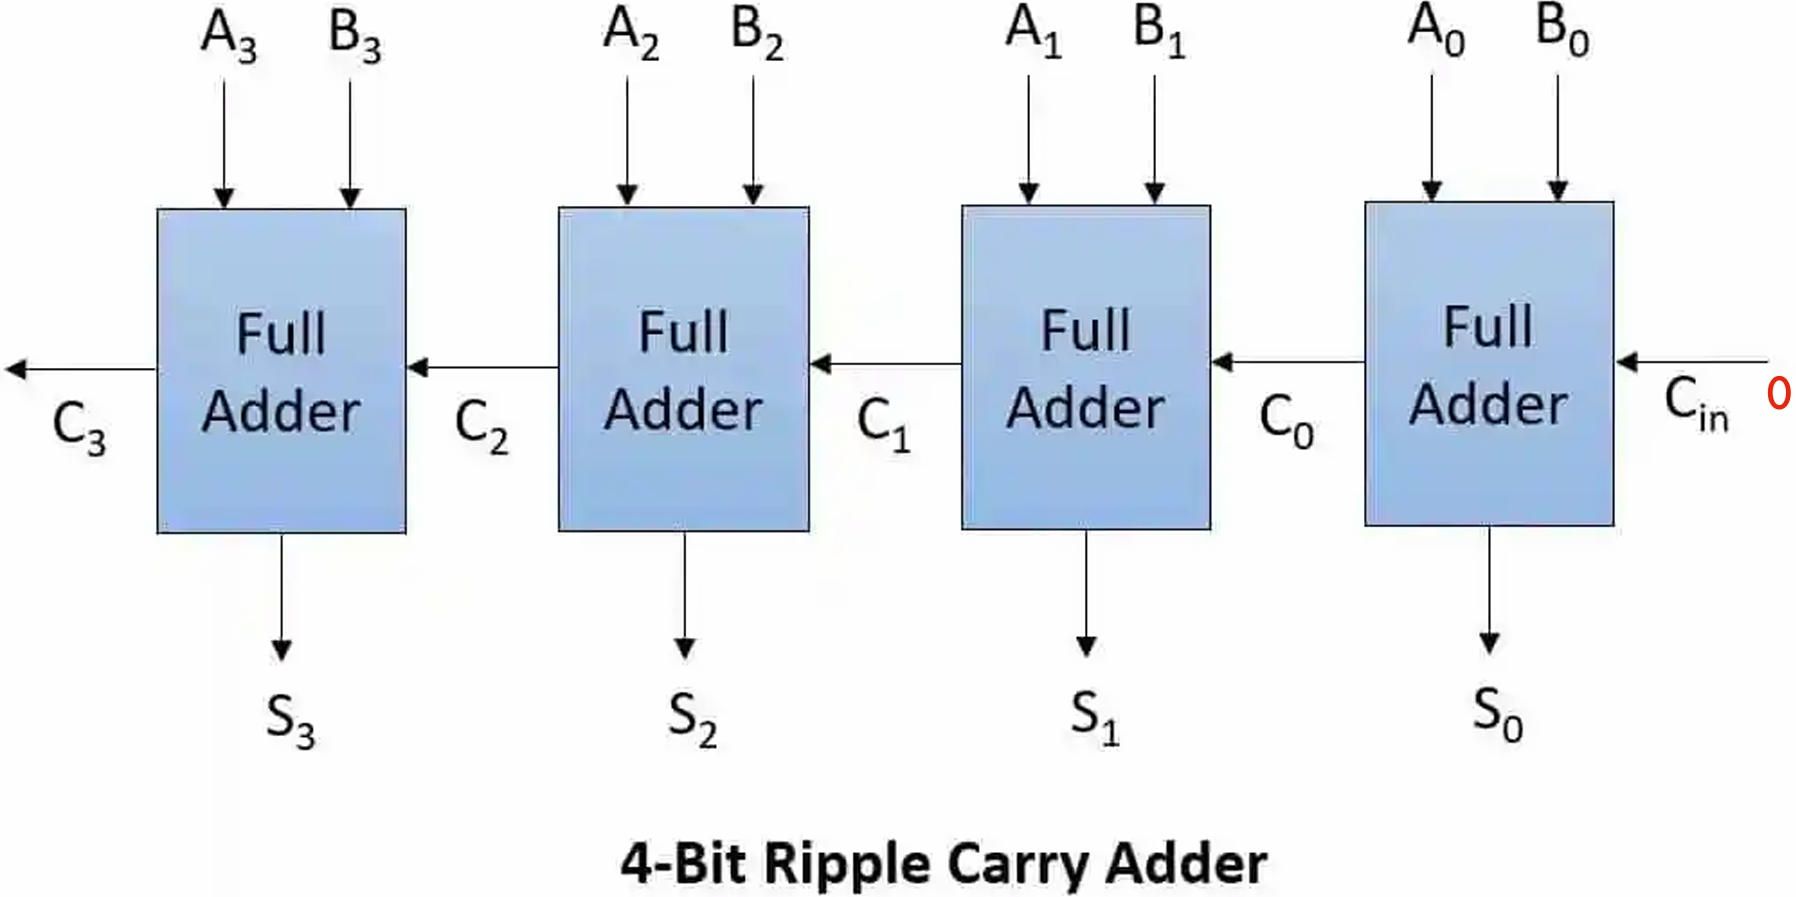
\includegraphics[scale = 0.18]{ch1/ch1_figure2.jpeg}
\end{center}
\subsection{Universality of NAND Gate}
Originally, we can use \textcolor{cyan}{AND}, \textcolor{cyan}{OR} and \textcolor{cyan}{NOT} gates to construct any logic circuit.\\
\fbox{
    \parbox{0.97\textwidth}{
        \textit{\textbf{Example:}} $f(a,b,c) = (a \land b \land \neg c) \lor (\neg a \land \neg b \land c) \lor (a \land \neg b \land c)$ can be constructed using AND, OR and NOT gates.\\
        From the truth table, we can see that $f(a,b,c) = 1$ when $(a,b,c) = (1, 1, 0)$, $(0, 0, 1)$ and $(1, 0, 1)$.
    }
}\\
\vspace{0.2cm}
However, we can also use \textcolor{cyan}{NAND} gates to construct any logic circuit.\\
\begin{enumerate}
    \item \textcolor{cyan}{NOT Gate}: \fbox{\textcolor{teal}{\(\text{NOT}(A) = \text{NAND}(A, A)\)}}
    \begin{center}
        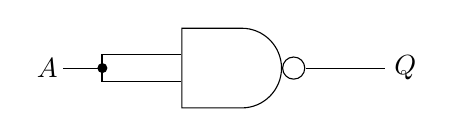
\begin{tikzpicture}
            \node[nand gate US, draw, rotate=0, logic gate inputs=nn, scale=2] at (0,0) (nand1) {};
            \draw (nand1.input 1) -- ++(-1,0) |- (nand1.input 2);
            \draw (nand1.output) -- ++(1,0) node[right] {\(Q\)};
            \node at (-2.3,0) {\(A\)};
            \draw (-2.1,0) to[short, -*] (-1.6,0);
        \end{tikzpicture}
    \end{center}
    \newpage
    \item \textcolor{cyan}{AND Gate}: \fbox{\textcolor{teal}{\(\text{AND}(A, B) = \text{NOT}(\text{NAND}(A, B))\)}}
    \begin{center}
        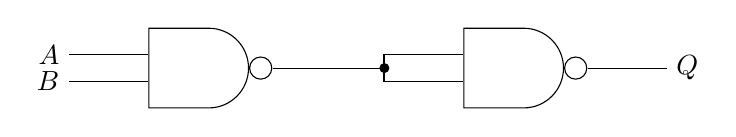
\begin{tikzpicture}
            \node[nand gate US, draw, rotate=0, logic gate inputs=nn, scale=2] at (0,0) (nand1) {};
            \node[nand gate US, draw, rotate=0, logic gate inputs=nn, scale=2] at (4,0) (nand2) {};
            \draw (nand2.input 1) -- ++(-1,0) |- (nand2.input 2);
            \draw (nand2.output) -- ++(1,0) node[right] {\(Q\)};
            \draw (nand1.input 1) -- ++(-1,0) node[left] {\(A\)};
            \draw (nand1.input 2) -- ++(-1,0) node[left] {\(B\)};
            \draw (nand1.output) to[short, -*] (2.4, 0);
        \end{tikzpicture}
    \end{center}
    \item \textcolor{cyan}{OR Gate}: \fbox{\textcolor{teal}{\(\text{OR}(A, B) = \text{NAND}(\text{NOT}(A), \text{NOT}(B))\)}}\\
    \begin{center}
        \begin{tikzpicture}
            \node[nand gate US, draw, rotate=0, logic gate inputs=nn, scale=2] at (0,0) (nand1) {};
            \node[nand gate US, draw, rotate=0, logic gate inputs=nn, scale=2] at (3,-1) (nand2) {};
            \node[nand gate US, draw, rotate=0, logic gate inputs=nn, scale=2] at (0,-2) (nand3) {};
            \draw (nand1.input 1) -- ++(-1,0) |- (nand1.input 2);
            \node (A) at (-2.9,0) {\(A\)};
            \draw (-2.6, 0) to [short, -*] (-1.6, 0);
            \draw (nand3.input 1) -- ++(-1,0) |- (nand3.input 2);
            \node (B) at (-2.9,-2) {\(B\)};
            \draw (-2.6, -2) to [short, -*] (-1.6, -2);
            \draw (nand1.output) -- ++(0.5,0) |- (nand2.input 1);
            \draw (nand3.output) -- ++(0.5,0) |- (nand2.input 2);
            \draw (nand2.output) -- ++(1,0) node[right] {\(Q\)};
        \end{tikzpicture}
    \end{center}
\end{enumerate}
Since \{AND, OR, NOT\} are universal, \textcolor{orange}{NAND gates are also universal} as they can be used to construct any logic circuit.
\textcolor{magenta}{\section{\textbf{Computer Science and Architecture}}}
\subsection{Turing Machine}
In 1936, \textcolor{cyan}{Alan Turing} introduced the concept of a Turing Machine as a mathematical model of computation and proved that universal computation can be achieved with a simple machine.\\
\begin{defBox}{Definition 1.2}{Turing Machine}
    \raggedright
    \textcolor{cyan}{Turing Machine} is a \textcolor{red}{simplified mathematical model} of a computer that can use for \textcolor{red}{general-purpose/universal computation}. \\
    It consists of an infinite tape divided into cells, a read/write head that can move left or right, and a finite set of states.
\end{defBox}
\uline{\textbf{Components of a Turing Machine}}:
\begin{itemize}
    \item \textcolor{gray}{Input:} \textcolor{blue}{A sequence of symbols on the infinite tape}.
    \item \textcolor{gray}{Rules:} \textcolor{blue}{A set of instructions for the read/write head to move left or right, read or write a symbol, and change state}.
    \item \textcolor{gray}{Output:} \textcolor{blue}{The result of the computation on the tape}.
\end{itemize}
Turing Machines nowadays can be applied in realizations of computers, games like Minecraft and Manufactoria (Puzzle Game) or Brainf**k Language Simulation.
\subsection{Von Neumann Architecture}
In 1945, \textcolor{cyan}{John von Neumann} proposed the concept of a stored-program computer, which is the basis of modern computer architecture.\\
\vspace{0.2cm}
\uline{\textbf{Components of a Von Neumann Architecture}}:
\begin{itemize}
    \item \textcolor{blue}{Central Processing Unit (CPU)}: \textcolor{forestgreen}{Performs arithmetic and logical operations} \& \textcolor{forestgreen}{Manages the data registers}.
    \item \textcolor{blue}{Memory}: \textcolor{forestgreen}{Stores data and programs}.
    \item \textcolor{blue}{Control Unit}: \textcolor{forestgreen}{Manages the instructions registers} \& \textcolor{forestgreen}{Acts as the program counter}.
    \item \textcolor{blue}{External Mass Storage}: \textcolor{forestgreen}{Stores large amounts of data}.
    \item \textcolor{blue}{Input/Output (I/O) Devices}: \textcolor{forestgreen}{Interacts with the user}.
\end{itemize}
\subsection{Random Access Memory (RAM)}
\begin{defBox}{Definition 1.3}{Random Access Memory (RAM)}
    \raggedright
    \textcolor{cyan}{Random Access Memory (RAM)} is a type of computer memory that can be \textcolor{red}{accessed at any memory location} and \textcolor{red}{quickly} by the CPU.\\
    $\implies$ \textcolor{purple}{Volatile} and \textcolor{purple}{Temporary}, meaning that the data is lost when the computer is turned off.
\end{defBox}
Since Turing Machines and Von Neumann Architecture read data sequentially, they are slow when accessing data stored at widely separated memory locations.\\
$\implies$ \textcolor{orange}{RAM is used to store data temporarily for quick access by the CPU}.
\newpage
\textcolor{magenta}{\section{\textbf{Reversible Computing}}}
\subsection{Landauer's Principle}
\begin{defBox}{Definition 1.4}{Landauer's Principle}
    \raggedright
    \textcolor{cyan}{Landauer's Principle} states that \textcolor{purple}{any logically irreversible operation like the erasure of 1 bit of information} must result in an \textcolor{purple}{increase in entropy and heat dissipation} in the physical system performing the computation.\\
    $\implies$ \textcolor{red}{Losing 1 bit of information dissipates \(k_BT \ln 2\) of energy}, where:
    \begin{itemize}
        \item \textcolor{brown}{\(k_B\)} is the Boltzmann constant.
        \item \textcolor{brown}{\(T\)} is the temperature (K).
    \end{itemize}
\end{defBox}
\begin{itemize}
    \item \uline{e.g.:} If $T = 300$ K, then the energy dissipated is \(k_BT \ln 2 \approx 2.9 \times 10^{-21}\) J.
\end{itemize}
\uline{\textbf{Information Erasure}}:\\
There are two cases for information erasure:
\begin{itemize}
    \item \textcolor{gray}{Case 1:} If \textcolor{forestgreen}{A bit has a value of 0/1 with probability of 50\%}, then we gain \textcolor{orange}{1 bit of information} when we measure the bit.
    \item \textcolor{gray}{Case 2:} If \textcolor{forestgreen}{A bit has a value of 0 with probability of 100\%}, then we gain \textcolor{orange}{0 bit of information} when we measure the bit.
\end{itemize}
\begin{thmBox}{Theorem 1.2}{Average Information Gain}
    \textcolor{cyan}{Average Information Gain} when measuring a bit if \textcolor{brown}{\(P[0] = p\)} and \textcolor{brown}{\(P[1] = 1 - p\)} is:
    \[
    \boxed{\textcolor{teal}{H_b(p) = -p \log_2(p) - (1 - p) \log_2(1 - p)}}
    \]
\end{thmBox}
\begin{egBox}{Example 1.11}{Average Information Lost of Irreversible NAND Gate}
    \raggedright
    Naively, the 2 input bits of a NAND gate will produce 1 output bit. $\implies$ Probability of output bit being 0 is $\frac{1}{4}$ and 1 is $\frac{3}{4}$.\\
    \vspace{1mm}
    Information in Output Bit: $H_b\left(\frac{1}{4}\right) = -\frac{1}{4} \log_2\left(\frac{1}{4}\right) - \frac{3}{4} \log_2\left(\frac{3}{4}\right) \approx 0.811$ bits.\\
    \vspace{1mm}
    $\therefore$ The average information lost for a NAND gate is:
    \[
    \text{Average Information Lost} = 2 - 0.811 \approx \underline{\underline{1.189 \text{ bits}}}
    \]
\end{egBox}
\textcolor{blue}{AND, OR, NAND, NOR, XOR and XNOR gates} are all irreversible, meaning these gates will \textcolor{orange}{lose information and dissipate heat} when performing computations.\\
As a result, we need to design reversible circuits to \textcolor{red}{have no heat dissipation due to information erasure}.
\subsection{Reversible Computing and Functions}
\begin{defBox}{Definition 1.5}{Reversible Computing}
    \raggedright
    \textcolor{cyan}{Reversible Computing} is a form of unconventional computing that \hl{performs reversible computation in the entire process}.\\
    $\implies$ \textcolor{red}{Each step of the computation implements a reversible function}.
\end{defBox}
\begin{defBox}{Definition 1.6}{Reversible Function}
    \raggedright
    A \textcolor{cyan}{reversible function} is a function that \textcolor{red}{is one-to-one/bijective} (Given the output $y$, we can uniquely determine the input $x$).
\end{defBox}
\textcolor{blue}{NOT gate} is an example of a reversible function as it is one-to-one.\\
\newpage
\subsection{Reversible Gates}
\begin{defBox}{Definition 1.7}{Reversible Gates}
    \raggedright
    \textcolor{cyan}{Reversible Gates} are logic gates that \textcolor{red}{implement reversible functions}.\\
    $\implies$ \textcolor{purple}{The number of input bits is equal to the number of output bits}.
\end{defBox}
There are several reversible gates that can be used to construct reversible circuits:
\begin{enumerate}
    \item \textcolor{blue}{Reversible XOR/Controlled NOT (CNOT) Gate}: \textcolor{teal}{\(\text{CNOT}(A, QB) = (A, A \oplus B) = (P, Q)\)}
    \begin{center}
        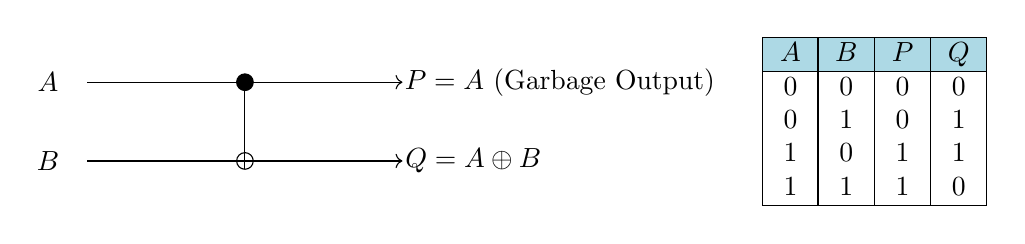
\begin{tikzpicture}
            \draw[->] (0, 1) -- (4, 1);
            \draw[->] (0, 0) -- (4, 0);
            \node at (-0.5, 1) {\(A\)};
            \node at (-0.5, 0) {\(B\)};
            \node at (6, 1) {\(P = A\) (Garbage Output)};
            \node at (4.9, 0) {\(Q = A \oplus B\)};
            \draw (2, 1) -- (2, -0.1);
            \filldraw[black] (2, 1) circle (3pt);
            \draw (2, 0) circle (3pt);

            \node at (10, 0.5) {\begin{tabular}{|c|c|c|c|}
                \hline
                \rowcolor{lightblue}
                \(A\) & \(B\) & \(P\) & \(Q\)\\
                \hline
                0 & 0 & 0 & 0\\
                0 & 1 & 0 & 1\\
                1 & 0 & 1 & 1\\
                1 & 1 & 1 & 0\\
                \hline
            \end{tabular}};
        \end{tikzpicture}
    \end{center}
    \item \textcolor{blue}{Toffoli Gate}: \textcolor{teal}{\(\text{TOF}(A, B, C) = (A, B, (A \land B) \oplus C) = (P, Q, R)\)}\\
    $\implies$ If \(C = 1\), then \(\text{TOF}(A, B, C) = (A, B, \text{NAND}(A, B))\) which is universal.
    \begin{center}
        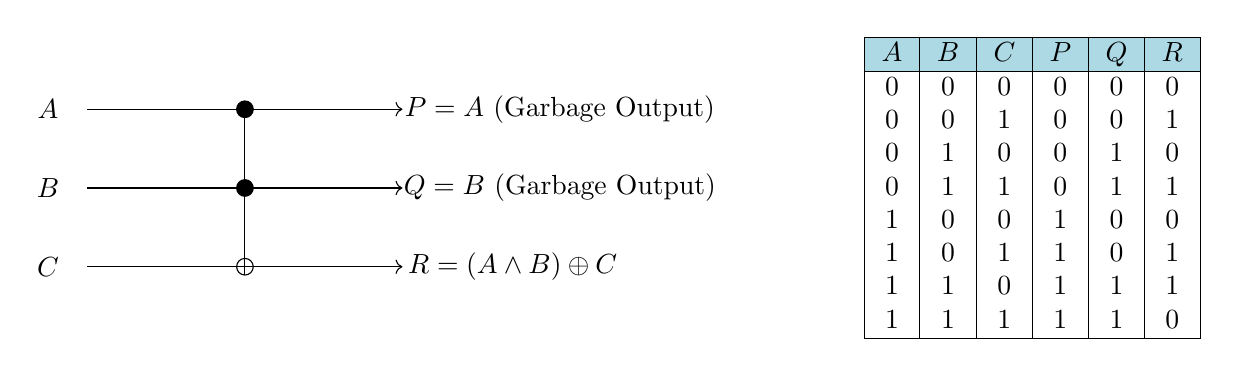
\begin{tikzpicture}
            \draw[->] (0, 3) -- (4, 3);
            \draw[->] (0, 2) -- (4, 2);
            \draw[->] (0, 1) -- (4, 1);
            \node at (-0.5, 3) {\(A\)};
            \node at (-0.5, 2) {\(B\)};
            \node at (-0.5, 1) {\(C\)};
            \node at (6, 3) {\(P = A\) (Garbage Output)};
            \node at (6, 2) {\(Q = B\) (Garbage Output)};
            \node at (5.4, 1) {\(R = (A \land B) \oplus C\)};
            \draw (2, 3) -- (2, 0.9);
            \filldraw[black] (2, 3) circle (3pt);
            \filldraw[black] (2, 2) circle (3pt);
            \draw (2, 1) circle (3pt);

            \node at (12, 2) {\begin{tabular}{|c|c|c|c|c|c|c|}
                \hline
                \rowcolor{lightblue}
                \(A\) & \(B\) & \(C\) & \(P\) & \(Q\) & \(R\)\\
                \hline
                0 & 0 & 0 & 0 & 0 & 0\\
                0 & 0 & 1 & 0 & 0 & 1\\
                0 & 1 & 0 & 0 & 1 & 0\\
                0 & 1 & 1 & 0 & 1 & 1\\
                1 & 0 & 0 & 1 & 0 & 0\\
                1 & 0 & 1 & 1 & 0 & 1\\
                1 & 1 & 0 & 1 & 1 & 1\\
                1 & 1 & 1 & 1 & 1 & 0\\
                \hline
            \end{tabular}};
        \end{tikzpicture}
    \end{center}
    \item \textcolor{blue}{Reversible Half Adder}: \textcolor{teal}{\(\text{Half Adder}(A, B) = (A \oplus B, A \land B) = (S, C_0)\)}
    \begin{center}
        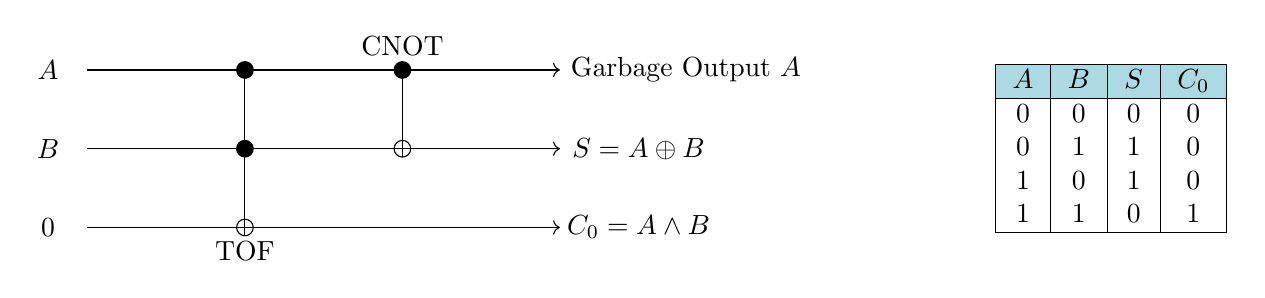
\begin{tikzpicture}
            \draw[->] (0, 1) -- (6, 1);
            \draw[->] (0, 0) -- (6, 0);
            \draw[->] (0, -1) -- (6, -1);
            \node at (-0.5, 1) {\(A\)};
            \node at (-0.5, 0) {\(B\)};
            \node at (-0.5, -1) {\(0\)};
            \node at (7.6, 1) {Garbage Output \(A\)};
            \node at (7, 0) {\(S = A \oplus B\)};
            \node at (7, -1) {\(C_0 = A \land B\)};
            \draw (2, 1) -- (2, -1.1);
            \filldraw[black] (2, 1) circle (3pt);
            \filldraw[black] (2, 0) circle (3pt);
            \draw (2, -1) circle (3pt);
            \draw (4, 1) -- (4, -0.1);
            \filldraw[black] (4, 1) circle (3pt);
            \draw (4, 0) circle (3pt);
            \node at (2, -1.3) {TOF};
            \node at (4, 1.3) {CNOT};


            \node at (13, 0) {\begin{tabular}{|c|c|c|c|}
                \hline
                \rowcolor{lightblue}
                \(A\) & \(B\) & \(S\) & \(C_0\)\\
                \hline
                0 & 0 & 0 & 0\\
                0 & 1 & 1 & 0\\
                1 & 0 & 1 & 0\\
                1 & 1 & 0 & 1\\
                \hline
            \end{tabular}};
        \end{tikzpicture}
    \end{center}
\end{enumerate}





\chapter{Brief Introduction to Quantum Computers}
\textcolor{magenta}{\section{\textbf{Quantum States}}}
\subsection{Quantization and Superposition}
\begin{defBox}{Definition 2.1}{Quantization}
    \raggedright
    \textcolor{cyan}{Quantization} is the process of \textcolor{red}{discretizing} a continuous variable into \textcolor{red}{quantum states $\ket{\psi}$}.
\end{defBox}
Differences between Classical Bits and Quantum Bits:
\begin{itemize}
    \item \textcolor{blue}{Classical Bit}: \textcolor{teal}{\(0\) or \(1\)}.
    \item \textcolor{blue}{Quantum Bit (Qubit)}: \textcolor{teal}{\(\ket{0}\) or \(\ket{1}\)}.
\end{itemize}
\begin{defBox}{Definition 2.2}{Superposition}
    \raggedright
    \textcolor{cyan}{Superposition} is the ability of a quantum system to combine multiple quantum states \(\ket{\psi}\) into a single quantum state.
\end{defBox}
\fbox{
    \parbox{0.97\textwidth}{
        \textit{\textbf{Remark:}} \\
        There is no $\ket{0} + \ket{1} = \ket{1}$ in quantum computing. $\implies$ Physical Meaning of Superposition: \textcolor{orange}{A combination of $\ket{0}$ and $\ket{1}$}.
    }
}
\subsection{State of a Qubit}
\begin{defBox}{Definition 2.3}{State of a Qubit}
    \raggedright
    The \textcolor{cyan}{state of a qubit} is a \textcolor{red}{superposition/combination} of the \textcolor{red}{basis states \(\ket{0}\) and \(\ket{1}\)}:
    \[
    \boxed{\textcolor{teal}{\ket{\psi} = \alpha \ket{0} + \beta \ket{1}}} \quad \text{where } \alpha \neq 0 \text{ or } \beta \neq 0
    \]
\end{defBox}
Examples of Qubit States with Different \(\alpha\) and \(\beta\):
\begin{itemize}
    \item \textcolor{gray}{\(\alpha = 1, \beta = 0\)}: \textcolor{forestgreen}{\(\ket{\psi} = 1 \ket{0} + 0 \ket{1} = \ket{0}\)}.
    \item \textcolor{gray}{\(\alpha = 0, \beta = 1\)}: \textcolor{forestgreen}{\(\ket{\psi} = 0 \ket{0} + 1 \ket{1} = \ket{1}\)}.
    \item \textcolor{gray}{\(\alpha = 1, \beta = 1\)}: \textcolor{forestgreen}{\(\ket{\psi} = 1 \ket{0} + 1 \ket{1} = \ket{0} + \ket{1}\)}.
    \item \textcolor{gray}{\(\alpha = 1, \beta = -1\)}: \textcolor{forestgreen}{\(\ket{\psi} = 1 \ket{0} - 1 \ket{1} = \ket{0} - \ket{1}\)}.
    \item \textcolor{blue}{All real numbers} $\implies$ \textcolor{gray}{\(\alpha = \sqrt{\frac{1}{10}}, \beta = -\sqrt{\frac{9}{10}}\)}: \textcolor{forestgreen}{\(\ket{\psi} = \sqrt{\frac{1}{10}} \ket{0} + \sqrt{\frac{9}{10}} \ket{1}\)}.
    \item \textcolor{blue}{All complex numbers} $\implies$ \textcolor{gray}{\(\alpha = 1, \beta = -j\)}: \textcolor{forestgreen}{\(\ket{\psi} = 1 \ket{0} - j \ket{1}\)}.
\end{itemize}
\subsection{Algebra of Qubit States}
Qubit states are \textcolor{cyan}{vectors} which can form a \textcolor{purple}{vector space}. \\
$\implies$ Therefore, they can perform vector operations such as \textcolor{cyan}{sclar multiplication} and \textcolor{cyan}{vector addition}.\\
\newpage
\uline{\textbf{Scalar Multiplication}}:
\begin{thmBox}{Theorem 2.1}{Scalar Multiplication of Qubit States}
    The \textcolor{cyan}{scalar multiplication} of a qubit state \textcolor{brown}{\(\ket{\psi} = \alpha \ket{0} + \beta \ket{1}\)} by a scalar \(\gamma\) is:
    \[
    \boxed{\textcolor{teal}{\gamma \ket{\psi} = \gamma \alpha \ket{0} + \gamma \beta \ket{1}}} \quad \text{where } \alpha, \beta, \gamma \in \mathbb{C}
    \]
\end{thmBox}
\begin{itemize}
    \item \uline{e.g.} \textcolor{gray}{\(\gamma = \frac{1}{\sqrt{2}}\)}: \textcolor{forestgreen}{\(\frac{1}{\sqrt{2}} \ket{\psi} = \frac{1}{\sqrt{2}} \alpha \ket{0} + \frac{1}{\sqrt{2}} \beta \ket{1}\)}.
\end{itemize}
\uline{\textbf{Vector Addition}}:
\begin{thmBox}{Theorem 2.2}{Vector Addition of Qubit States}
    The \textcolor{cyan}{vector addition} of two qubit states \textcolor{brown}{\(\ket{\psi_1} = \alpha_1 \ket{0} + \beta_1 \ket{1}\)} and \textcolor{brown}{\(\ket{\psi_2} = \alpha_2 \ket{0} + \beta_2 \ket{1}\)} is:
    \[
    \boxed{\textcolor{teal}{\ket{\psi_1} + \ket{\psi_2} = (\alpha_1 + \alpha_2) \ket{0} + (\beta_1 + \beta_2) \ket{1}}} \quad \text{where } \alpha_1, \alpha_2, \beta_1, \beta_2 \in \mathbb{C}
    \]
\end{thmBox}
Combing both scalar multiplication and vector addition, we can perform the following operations:
\[
    \boxed{c_1(\alpha_1 \ket{0} + \beta_1 \ket{1}) + c_2(\alpha_2 \ket{0} + \beta_2 \ket{1}) = (\alpha_1 c_1 + \alpha_2 c_2) \ket{0} + (\beta_1 c_1 + \beta_2 c_2) \ket{1}}
\]
\begin{itemize}
    \item \uline{e.g.} \textcolor{forestgreen}{\(\frac{1}{2} (\ket{0} + \ket{1}) + \frac{1}{2} (\ket{0} - \ket{1}) = \frac{1}{2} \ket{0} + \frac{1}{2} \ket{1} + \frac{1}{2} \ket{0} - \frac{1}{2} \ket{1} = \ket{0}\)}.
\end{itemize}
\fbox{
    \parbox{0.97\textwidth}{
        \textit{\textbf{Remark:}} Do not write \(\alpha \ket{0} + \beta \ket{1} \) in other courses as vector operations.
    }
}\\
\textcolor{magenta}{\section{\textbf{Single-Qubit Gates}}}
\subsection{Quantum Gates}
\begin{defBox}{Definition 2.4}{Quantum Gates}
    \raggedright
    \textcolor{cyan}{Quantum Gates} are \textcolor{red}{unitary operators} that \textcolor{red}{operate on qubit states} to perform quantum computations.\\
    $\implies$ Function $U(\cdot)$ takes a qubit state $\ket{\psi}$ and outputs a new qubit state $U(\ket{\psi})$.
    \begin{center}
        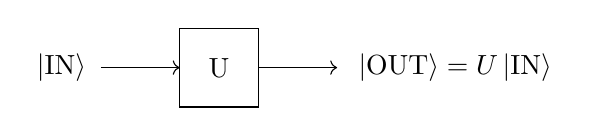
\begin{tikzpicture}
            \draw (0,0) rectangle (1,1) node[midway] {U};
            \draw[->] (-1,0.5) -- (0,0.5);
            \node at (-1.5, 0.5) {$\ket{\text{IN}}$};
            \draw[->] (1,0.5) -- (2,0.5);
            \node at (3.5,0.5) {$\ket{\text{OUT}} = U \ket{\text{IN}}$};
        \end{tikzpicture}
    \end{center}
\end{defBox}
Linearity of Quantum Gates: \textcolor{forestgreen}{\(U \left( U(\alpha \ket{\psi_1} + \beta \ket{\psi_2}) \right) = \alpha U(\ket{\psi_1}) + \beta U(\ket{\psi_2})\)}.
\begin{center}
    \begin{tikzpicture}
        \draw (0,0) rectangle (1,1) node[midway] {U};
        \draw[->] (-1,0.5) -- (0,0.5);
        \node at (-1.3, 0.5) {$\ket{\text{0}}$};
        \draw[->] (1,0.5) -- (2,0.5);
        \node at (2.5,0.5) {$U \ket{\text{0}}$};

        \draw (6,0) rectangle (7,1) node[midway] {U};
        \draw[->] (5,0.5) -- (6,0.5);
        \node at (4.7, 0.5) {$\ket{\text{1}}$};
        \draw[->] (7,0.5) -- (8,0.5);
        \node at (8.5,0.5) {$U \ket{\text{1}}$};

        \draw (3,-2) rectangle (4,-1) node[midway] {U};
        \draw[->] (2,-1.5) -- (3,-1.5);
        \node at (1, -1.5) {$\alpha \ket{\text{0}} + \beta \ket{\text{1}}$};
        \draw[->] (4,-1.5) -- (5,-1.5);
        \node at (6.3,-1.5) {$\alpha U \ket{\text{0}} + \beta U \ket{\text{1}}$};
    \end{tikzpicture}
\end{center}
\fbox{
    \parbox{0.97\textwidth}{
        \textit{\textbf{Remark:}} \textcolor{orange}{Quantum Gates are reversible} as they are unitary operators.
    }
}\\
\subsection{Types of Single-Qubit Gates}
There are several types of single-qubit gates that can be used to perform quantum computations:
\begin{enumerate}
    \item \textcolor{blue}{Identity Gates}: \textcolor{teal}{\(\ket{0} \rightarrow \ket{0}\)} and \textcolor{teal}{\(\ket{1} \rightarrow \ket{1}\)}.
    \begin{center}
        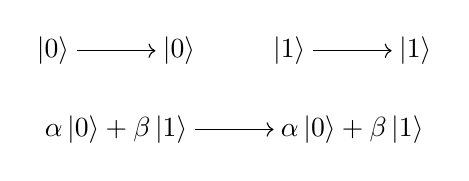
\begin{tikzpicture}
            \draw[->] (0,0) -- (1,0);
            \node at (-0.3,0) {\(\ket{0}\)};
            \node at (1.3,0) {\(\ket{0}\)};

            \draw[->] (3,0) -- (4,0);
            \node at (2.7,0) {\(\ket{1}\)};
            \node at (4.3,0) {\(\ket{1}\)};

            \draw[->] (1.5, -1) -- (2.5, -1);
            \node at (0.5,-1) {\(\alpha \ket{0} + \beta \ket{1}\)};
            \node at (3.5,-1) {\(\alpha \ket{0} + \beta \ket{1}\)};
        \end{tikzpicture}
    \end{center}
    \newpage
    \item \textcolor{blue}{X Gate} (Bit-Flip Gate): \textcolor{teal}{\(\ket{0} \rightarrow \ket{1}\)} and \textcolor{teal}{\(\ket{1} \rightarrow \ket{0}\)}
    \begin{center}
        \begin{tikzpicture}
            \draw (0,0) rectangle (1,1) node[midway] {X};
            \draw[->] (-1,0.5) -- (0,0.5);
            \node at (-1.3, 0.5) {$\ket{\text{0}}$};
            \draw[->] (1,0.5) -- (2,0.5);
            \node at (2.3,0.5) {$\ket{\text{1}}$};
    
            \draw (6,0) rectangle (7,1) node[midway] {X};
            \draw[->] (5,0.5) -- (6,0.5);
            \node at (4.7, 0.5) {$\ket{\text{1}}$};
            \draw[->] (7,0.5) -- (8,0.5);
            \node at (8.3,0.5) {$\ket{\text{0}}$};
    
            \draw (3,-2) rectangle (4,-1) node[midway] {X};
            \draw[->] (2,-1.5) -- (3,-1.5);
            \node at (1, -1.5) {$\alpha \ket{\text{0}} + \beta \ket{\text{1}}$};
            \draw[->] (4,-1.5) -- (5,-1.5);
            \node at (6,-1.5) {$\alpha \ket{\text{1}} + \beta \ket{\text{0}}$};
        \end{tikzpicture}
    \end{center}
    \begin{itemize}
        \item \uline{e.g. 1:} \textcolor{gray}{\(\alpha = \frac{1}{\sqrt{2}}, \beta = \frac{1}{\sqrt{2}}\)}: \textcolor{forestgreen}{\(\ket{\psi} = \frac{1}{\sqrt{2}} \ket{0} + \frac{1}{\sqrt{2}} \ket{1}\)}.
        \item \uline{e.g. 2:} \textcolor{gray}{\(\alpha = \frac{1}{\sqrt{2}}, \beta = -\frac{1}{\sqrt{2}}\)}: \textcolor{forestgreen}{\(\ket{\psi} = \frac{1}{\sqrt{2}} \ket{0} - \frac{1}{\sqrt{2}} \ket{1}\)}.
    \end{itemize}
    \item \textcolor{blue}{Z Gate} (Phase-Flip Gate): \textcolor{teal}{\(\ket{0} \rightarrow \ket{0}\)} and \textcolor{teal}{\(\ket{1} \rightarrow -\ket{1}\)}
    \begin{center}
        \begin{tikzpicture}
            \draw (0,0) rectangle (1,1) node[midway] {Z};
            \draw[->] (-1,0.5) -- (0,0.5);
            \node at (-1.3, 0.5) {$\ket{\text{0}}$};
            \draw[->] (1,0.5) -- (2,0.5);
            \node at (2.3,0.5) {$\ket{\text{0}}$};
    
            \draw (6,0) rectangle (7,1) node[midway] {Z};
            \draw[->] (5,0.5) -- (6,0.5);
            \node at (4.7, 0.5) {$\ket{\text{1}}$};
            \draw[->] (7,0.5) -- (8,0.5);
            \node at (8.4,0.5) {$-\ket{\text{1}}$};
    
            \draw (3,-2) rectangle (4,-1) node[midway] {Z};
            \draw[->] (2,-1.5) -- (3,-1.5);
            \node at (1, -1.5) {$\alpha \ket{\text{0}} + \beta \ket{\text{1}}$};
            \draw[->] (4,-1.5) -- (5,-1.5);
            \node at (6,-1.5) {$\alpha \ket{\text{0}} - \beta \ket{\text{1}}$};
        \end{tikzpicture}
    \end{center}
    \begin{itemize}
        \item \uline{e.g. 1:} \textcolor{gray}{\(\alpha = \frac{1}{\sqrt{2}}, \beta = \frac{1}{\sqrt{2}}\)}: \textcolor{forestgreen}{\(\ket{\psi} = \frac{1}{\sqrt{2}} \ket{0} - \frac{1}{\sqrt{2}} \ket{1}\)}.
        \item \uline{e.g. 2:} \textcolor{gray}{\(\alpha = \frac{1}{\sqrt{2}}, \beta = -\frac{1}{\sqrt{2}}\)}: \textcolor{forestgreen}{\(\ket{\psi} = \frac{1}{\sqrt{2}} \ket{0} + \frac{1}{\sqrt{2}} \ket{1}\)}.
    \end{itemize}
    \item \textcolor{blue}{H Gate} (Hadamard Gate): \textcolor{teal}{\(\ket{0} \rightarrow \frac{1}{\sqrt{2}}\ket{0} + \frac{1}{\sqrt{2}}\ket{1}\)} and \textcolor{teal}{\(\ket{1} \rightarrow \frac{1}{\sqrt{2}}\ket{0} - \frac{1}{\sqrt{2}}\ket{1}\)}
    \begin{center}
        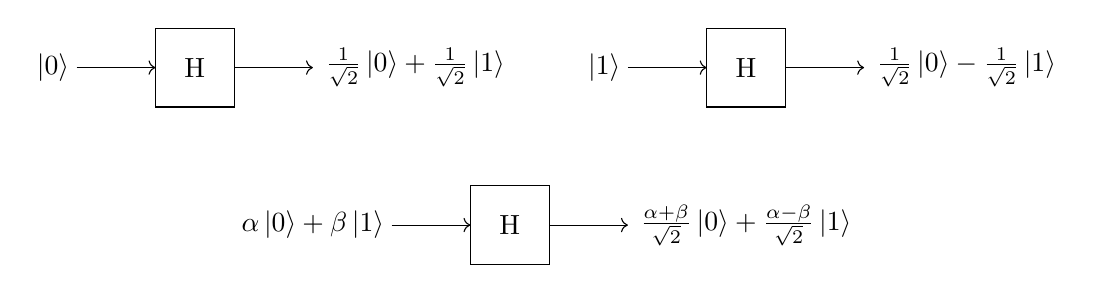
\begin{tikzpicture}
            \draw (0,0) rectangle (1,1) node[midway] {H};
            \draw[->] (-1,0.5) -- (0,0.5);
            \node at (-1.3, 0.5) {$\ket{\text{0}}$};
            \draw[->] (1,0.5) -- (2,0.5);
            \node at (3.3,0.5) {\(\frac{1}{\sqrt{2}}\ket{\text{0}} + \frac{1}{\sqrt{2}}\ket{\text{1}}\)};
    
            \draw (7,0) rectangle (8,1) node[midway] {H};
            \draw[->] (6,0.5) -- (7,0.5);
            \node at (5.7, 0.5) {$\ket{\text{1}}$};
            \draw[->] (8,0.5) -- (9,0.5);
            \node at (10.3,0.5) {\(\frac{1}{\sqrt{2}}\ket{\text{0}} - \frac{1}{\sqrt{2}}\ket{\text{1}}\)};
    
            \draw (4,-2) rectangle (5,-1) node[midway] {H};
            \draw[->] (3,-1.5) -- (4,-1.5);
            \node at (2, -1.5) {$\alpha \ket{\text{0}} + \beta \ket{\text{1}}$};
            \draw[->] (5,-1.5) -- (6,-1.5);
            \node at (7.5,-1.5) {\(\frac{\alpha + \beta}{\sqrt{2}}\ket{\text{0}} + \frac{\alpha - \beta}{\sqrt{2}}\ket{\text{1}}\)};
        \end{tikzpicture}
    \end{center}
    \begin{itemize}
        \item \uline{e.g. 1:} \textcolor{gray}{\(\alpha = \frac{1}{\sqrt{2}}, \beta = \frac{1}{\sqrt{2}}\)}: \textcolor{forestgreen}{\(\ket{\psi} = \frac{\frac{1}{\sqrt{2}} + \frac{1}{\sqrt{2}}}{\sqrt{2}} \ket{0} + \frac{\frac{1}{\sqrt{2}} - \frac{1}{\sqrt{2}}}{\sqrt{2}} \ket{1} = \ket{0}\)}.
        \item \uline{e.g. 2:} \textcolor{gray}{\(\alpha = \frac{1}{\sqrt{2}}, \beta = -\frac{1}{\sqrt{2}}\)}: \textcolor{forestgreen}{\(\ket{\psi} = \frac{\frac{1}{\sqrt{2}} - \frac{1}{\sqrt{2}}}{\sqrt{2}} \ket{0} + \frac{\frac{1}{\sqrt{2}} + \frac{1}{\sqrt{2}}}{\sqrt{2}} \ket{1} = \ket{1}\)}.
    \end{itemize}
\end{enumerate}
They are \textcolor{red}{all reversible} as they are unitary operators.\\
\textcolor{magenta}{\section{\textbf{Multi-Qubit States and Gates}}}
\subsection{Two-Qubit States}
\begin{defBox}{Definition 2.5}{Two-Qubit States}
    \raggedright
    The \textcolor{cyan}{state of two qubits} is a \textcolor{red}{superposition/combination} of the \hl{basis states of 2 classical bits} \textcolor{red}{ \(\ket{00}, \ket{01}, \ket{10}, \ket{11}\)}:
    \[
    \boxed{\textcolor{teal}{\ket{\psi} = c_{00} \ket{00} + c_{01} \ket{01} + c_{10} \ket{10} + c_{11} \ket{11}}} \quad \text{where } c_{00}, c_{01}, c_{10}, c_{11} \text{ are complex numbers}
    \]
\end{defBox}
\uline{\textbf{Joint State of Two Qubits}}
\begin{thmBox}{Theorem 2.3}{Joint State of Two Qubits}
    The \textcolor{cyan}{joint state of two qubits} is the \textcolor{red}{tensor product ($\otimes$)} of the \textcolor{red}{individual qubit states} \textcolor{brown}{\(\ket{\psi_1} = \alpha_1 \ket{0} + \beta_1 \ket{1}\)} and \textcolor{brown}{\(\ket{\psi_2} = \alpha_2 \ket{0} + \beta_2 \ket{1}\)}:
    \begin{center}
        \fbox{
            \textcolor{teal}{
            \(
            \begin{aligned}
            \ket{\psi} &= \ket{\psi_1} \otimes \ket{\psi_2} \\
            &= (\alpha_1 \ket{0} + \beta_1 \ket{1}) \otimes (\alpha_2 \ket{0} + \beta_2 \ket{1}) \\
            &= \alpha_1 \alpha_2 \ket{00} + \alpha_1 \beta_2 \ket{01} + \beta_1 \alpha_2 \ket{10} + \beta_1 \beta_2 \ket{11}
            \end{aligned}
            \)
            }
        }
    \end{center}
\end{thmBox}
\newpage
Examples of Joint States of Two Qubits (Sometimes omit the tensor product symbol):
\begin{itemize}
    \item \textcolor{gray}{\(\alpha_1 = \alpha_2 = 1, \beta_1 = \beta_2 = 0\)}: \textcolor{forestgreen}{\(\ket{\psi} = \ket{0} \otimes \ket{0} = \ket{00}\)}.
    \item \textcolor{gray}{\(\alpha_1 = \beta_2 = 1, \beta_1 = \alpha_2 = 0\)}: \textcolor{forestgreen}{\(\ket{\psi} = \ket{0} \otimes \ket{1} = \ket{01}\)}.
    \item \textcolor{gray}{\(\beta_1 = \alpha_2 = 1, \alpha_1 = \beta_2 = 0\)}: \textcolor{forestgreen}{\(\ket{\psi} = \ket{1} \otimes \ket{0} = \ket{10}\)}.
    \item \textcolor{gray}{\(\beta_1 = \beta_2 = 1, \alpha_1 = \alpha_2 = 0\)}: \textcolor{forestgreen}{\(\ket{\psi} = \ket{1} \otimes \ket{1} = \ket{11}\)}.
\end{itemize}
\uline{\textbf{Properties of Two-Qubit States}}\\
Distribution Law of Tensor Product: \textcolor{blue}{\(\ket{A} \otimes (\ket{B} + \ket{C}) = \ket{A} \otimes \ket{B} + \ket{A} \otimes \ket{C}\)} or \textcolor{blue}{\((\ket{A} + \ket{B}) \otimes \ket{C} = \ket{A} \otimes \ket{C} + \ket{B} \otimes \ket{C}\)}.
\begin{itemize}
    \item \uline{e.g. 1:} \textcolor{forestgreen}{\((\ket{0} + \ket{1}) \otimes (\ket{0} + \ket{1}) = \ket{0} \otimes \ket{0} + \ket{0} \otimes \ket{1} + \ket{1} \otimes \ket{0} + \ket{1} \otimes \ket{1}\) = \(\ket{00} + \ket{01} + \ket{10} + \ket{11}\)}.
    \item \uline{e.g. 2:} \textcolor{forestgreen}{\((\ket{0} + \ket{1}) \otimes (\ket{0} - \ket{1}) = \ket{0} \otimes \ket{0} - \ket{0} \otimes \ket{1} + \ket{1} \otimes \ket{0} - \ket{1} \otimes \ket{1}\) = \(\ket{00} - \ket{01} + \ket{10} - \ket{11}\)}.
\end{itemize}
Linearity of Tensor Product: \textcolor{blue}{\(\alpha \ket{A} + \beta \ket{B} = \ket{A} \otimes (\alpha \ket{B}) = \alpha (\ket{A} \otimes \ket{B})\)}.\\
Communative Property of Tensor Product: \textcolor{blue}{\(\ket{A} \otimes \ket{B} = \ket{B} \otimes \ket{A}\)}.
\subsection{N-Qubit States}
\begin{defBox}{Definition 2.6}{N-Qubit States}
    \raggedright
    The \textcolor{cyan}{state of N qubits} is a \textcolor{red}{superposition/combination} of the \hl{basis states of N classical bits} \textcolor{red}{$\{0, 1\}^N$}:
    \[
    \boxed{\textcolor{teal}{\ket{\psi} = \sum_{s \in \{0, 1\}^N} c_s \ket{s}}} \quad \text{where } c_s \text{ are } 2^N \text{ complex numbers}
    \]
\end{defBox}
Example of N-Qubit States: \textcolor{forestgreen}{\(\ket{\psi} = \ket{0...0} + \ket{0...01} + \ldots + \ket{1...1} = (\ket{0} + \ket{1})^{\otimes N}\)}.
\subsection{Multi-Qubit Gates}
There are several types of multi-qubit gates that can be used to perform quantum computations:
\begin{enumerate}
    \item \textcolor{blue}{Controlled-X (CNOT) Gate}: First qubit is the control qubit and the second qubit is the target qubit.\\
    $\implies$ \textcolor{teal}{$\text{CNOT}\ket{00} = \ket{00}$}, \textcolor{teal}{$\text{CNOT}\ket{01} = \ket{01}$}, \textcolor{teal}{$\text{CNOT}\ket{10} = \ket{11}$}, \textcolor{teal}{$\text{CNOT}\ket{11} = \ket{10}$}.
    \begin{center}
        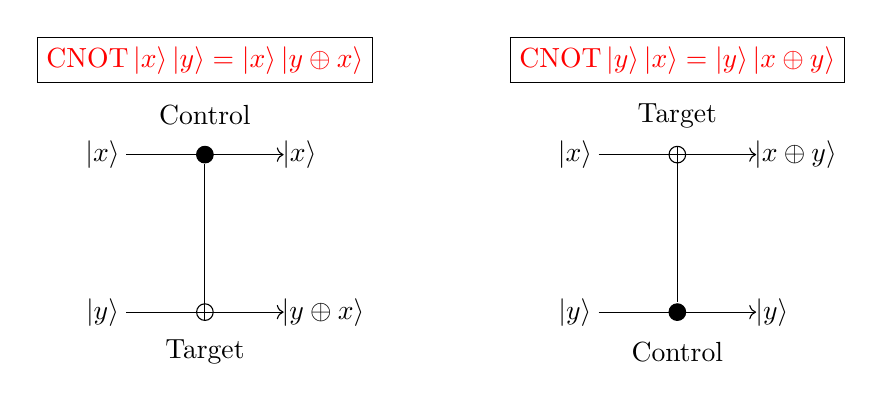
\begin{tikzpicture}
            \node at (0, 1.2) {$\boxed{\textcolor{red}{\text{CNOT}\ket{x}\ket{y} = \ket{x}\ket{y \oplus x}}}$};
            \node at (0,0) (control) {};
            \node at (0,-2) (target) {};
            \draw (control) -- (0, -2.1);
            \filldraw[black] (control) circle (3pt);
            \draw (target) circle (3pt);
            \draw [->] (-1, 0) -- (1, 0);
            \draw [->] (-1, -2) -- (1, -2);
            \node at (-1.3, 0) {\(\ket{x}\)};
            \node at (-1.3, -2) {\(\ket{y}\)};
            \node at (1.2, 0) {\(\ket{x}\)};
            \node at (1.5, -2) {\(\ket{y \oplus x}\)};
            \node at (0, 0.5) {Control};
            \node at (0, -2.5) {Target};

            \node at (6, 1.2) {$\boxed{\textcolor{red}{\text{CNOT}\ket{y}\ket{x} = \ket{y}\ket{x \oplus y}}}$};
            \node at (6, 0) (target2){};
            \node at (6, -2) (control2){};
            \draw (6, 0.1) -- (control2);
            \draw (target2) circle (3pt);
            \filldraw[black] (control2) circle (3pt);
            \draw [->] (5, 0) -- (7, 0);
            \draw [->] (5, -2) -- (7, -2);
            \node at (4.7, 0) {\(\ket{x}\)};
            \node at (4.7, -2) {\(\ket{y}\)};
            \node at (7.5, 0) {\(\ket{x \oplus y}\)};
            \node at (7.2, -2) {\(\ket{y}\)};
            \node at (6, 0.5) {Target};
            \node at (6, -2.5) {Control};
        \end{tikzpicture}
    \end{center}
    \begin{itemize}
        \item \uline{e.g.:} \begin{align*}
            \text{CNOT}(c_{00}\ket{00} + c_{01}\ket{01} + c_{10}\ket{10} + c_{11}\ket{11}) &= c_{00}\text{CNOT}\ket{00} + c_{01}\text{CNOT}\ket{01} + c_{10}\text{CNOT}\ket{10} + c_{11}\text{CNOT}\ket{11} \\
            &= c_{00}\ket{00} + c_{01}\ket{01} + \textcolor{orange}{c_{10}\ket{11}} + \textcolor{orange}{c_{11}\ket{10}}
        \end{align*}
    \end{itemize}
    \item \textcolor{blue}{1-Qubit Gates on Multi-Qubit States}: Apply the 1-qubit gate to the target qubit.
    \begin{itemize}
        \item \uline{e.g. 1:} If we apply the U gate to the first bit of the 2-qubit state \(\ket{\psi} = c_{00}\ket{00} + c_{01}\ket{01} + c_{10}\ket{10} + c_{11}\ket{11}\), we get:
        \begin{align*}
            & c_{00}(U\ket{0})\ket{0} + c_{01}(U\ket{0})\ket{1} + c_{10}(U\ket{1})\ket{0} + c_{11}(U\ket{1})\ket{1} \\
            &= U\ket{0} \otimes (c_{00}\ket{0} + c_{01}\ket{1}) + U\ket{1} \otimes (c_{10}\ket{0} + c_{11}\ket{1})
        \end{align*}
        \item \uline{e.g. 2:} If we apply the U gate to the second bit of the 2-qubit state \(\ket{\psi} = c_{00}\ket{00} + c_{01}\ket{01} + c_{10}\ket{10} + c_{11}\ket{11}\), we get:
        \begin{align*}
            & c_{00}\ket{0}(U\ket{0}) + c_{01}\ket{0}(U\ket{1}) + c_{10}\ket{1}(U\ket{0}) + c_{11}\ket{1}(U\ket{1}) \\
            &= (c_{00}\ket{0} + c_{10}\ket{1}) \otimes U\ket{0} + (c_{01}\ket{0} + c_{11}\ket{1}) \otimes U\ket{1}
        \end{align*}
    \end{itemize}
    \newpage
    \item \textcolor{blue}{3-Qubit Toffoli Gate}: First two qubits are control qubits and the third qubit is the target qubit.
    \[
        \boxed{\textcolor{red}{\text{TOF}\ket{x, y, z} = \ket{x, y, z}}} \quad \text{if } x, y \neq 1
    \]
    \[
        \boxed{\textcolor{red}{\text{TOF}\ket{x, y, z} = \ket{x, y, z \oplus x \land y}}} \quad \text{if } x, y = 1
    \]
    \begin{center}
        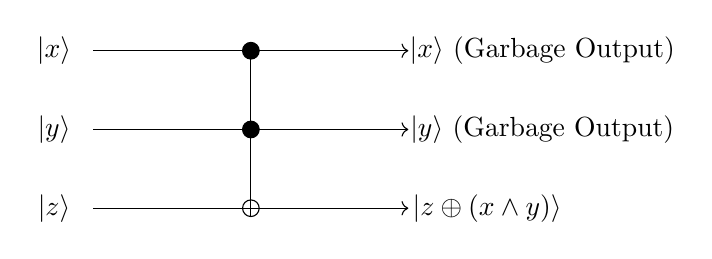
\begin{tikzpicture}
            \draw[->] (0, 3) -- (4, 3);
            \draw[->] (0, 2) -- (4, 2);
            \draw[->] (0, 1) -- (4, 1);
            \node at (-0.5, 3) {\(\ket{x}\)};
            \node at (-0.5, 2) {\(\ket{y}\)};
            \node at (-0.5, 1) {\(\ket{z}\)};
            \node at (5.7, 3) {\(\ket{x}\) (Garbage Output)};
            \node at (5.7, 2) {\(\ket{y}\) (Garbage Output)};
            \node at (5, 1) {\(\ket{z \oplus (x \land y)}\)};
            \draw (2, 3) -- (2, 0.9);
            \filldraw[black] (2, 3) circle (3pt);
            \filldraw[black] (2, 2) circle (3pt);
            \draw (2, 1) circle (3pt);
        \end{tikzpicture}
    \end{center}
    \begin{itemize}
        \item \uline{e.g.:} \(\text{TOF}(\ket{010} + \ket{110}) = \ket{010} + \ket{111}\).
    \end{itemize}
\end{enumerate}
\textcolor{magenta}{\section{\textbf{Measurement of Quantum Outputs}}}
\begin{defBox}{Definition 2.7}{Measurement of Quantum Outputs}
    \raggedright
    The \textcolor{cyan}{measurement of quantum outputs} is the process of \textcolor{red}{extracting classical information} from a quantum state.\\
    $\implies$ The \textcolor{red}{quantum state collapses} to one of the \textcolor{red}{basis states} \textcolor{brown}{\(\ket{0}, \ket{1}\)}.
\end{defBox}
\subsection{Single-Qubit Measurement}
\begin{thmBox}{Theorem 2.4}{Measurement of a Qubit State}
    The \textcolor{cyan}{measurement of a qubit state} \textcolor{brown}{\(\ket{\psi} = \alpha \ket{0} + \beta \ket{1}\)} results in:
    \begin{align*}
        & \text{Probability of Output Classical 0: } \boxed{\textcolor{teal}{P[0] = \frac{|\alpha|^2}{|\alpha|^2 + |\beta|^2}}} \\
        & \text{Probability of Output Classical 1: } \boxed{\textcolor{teal}{P[1] = \frac{|\beta|^2}{|\alpha|^2 + |\beta|^2}}} 
    \end{align*}
\end{thmBox}
\begin{itemize}
    \item \uline{e.g.:} For  \(\ket{\psi} = 4\ket{0} + 3\ket{1}\), the probability of measuring 0 is \(\frac{16}{25}\) and the probability of measuring 1 is \(\frac{9}{25}\).
\end{itemize}
There are different situations that can occur when measuring a qubit state:
\begin{enumerate}
    \item For real numbers, \(|\alpha|^2 = \alpha^2\) and \(|\beta|^2 = \beta^2\).
    \item For complex numbers, \(|\alpha|^2 = \alpha \cdot \alpha^* = |\alpha|^2\) and \(|\beta|^2 = \beta \cdot \beta^* = |\beta|^2\).
    \item If \(\ket{\psi} = \ket{0}\), then \(P[0] = 1\) and \(P[1] = 0\).
    \item If \(\ket{\psi} = \ket{1}\), then \(P[0] = 0\) and \(P[1] = 1\).
    \item If \(\ket{\psi} = \frac{1}{\sqrt{2}}(\ket{0} + \ket{1})\) or \(\ket{\psi} = \frac{1}{\sqrt{2}}(\ket{0} - \ket{1})\), then \(P[0] = P[1] = \frac{1}{2}\).
\end{enumerate}
\textcolor{purple}{Qubit States cannot be remeasured} as \hl{the qubit will be destroyed} after the first measurement.\\
\subsection{Two-Qubit Measurement}
\begin{thmBox}{Theorem 2.5}{Measurement of a Two-Qubit State}
    The \textcolor{cyan}{measurement of a two-qubit state} \textcolor{brown}{\(\ket{\psi} = c_{00}\ket{00} + c_{01}\ket{01} + c_{10}\ket{10} + c_{11}\ket{11}\)} results in:
    \begin{align*}
        & \text{Probability of Output } x_0x_1: \boxed{\textcolor{teal}{P[x_0x_1] = \frac{|c_{x_0x_1}|^2}{\sum_{y_0y_1} |c_{y_0y_1}|^2}}} \quad \text{where } x_0, x_1 \in \{0, 1\}
    \end{align*}
\end{thmBox}
\begin{itemize}
    \item \uline{e.g.:} For \(\ket{\psi} = \sqrt{3} \ket{00} + \sqrt{2} \ket{01} + \sqrt{5} \ket{10} + \sqrt{7} \ket{11}\), the probability of measuring 00 is \(\frac{3}{17}\), 01 is \(\frac{2}{17}\), 10 is \(\frac{5}{17}\), and 11 is \(\frac{7}{17}\).
\end{itemize}
\newpage
\subsection{Difference between Classical and Quantum Measurements}
\begin{center}
    \begin{tabular}{|c|c|c|}
        \hline
        \rowcolor{lightblue}
        & \textbf{Classical Measurement} & \textbf{Quantum Measurement} \\      \hline
        \textcolor{red}{\textbf{Output}} & \textcolor{teal}{Deterministic} & \textcolor{teal}{Probabilistic} \\
        \hline
        \textcolor{red}{\textbf{Reusability}} & \textcolor{teal}{Yes} & \textcolor{teal}{No} \\
        \hline
        \textcolor{red}{\textbf{Information}} & \textcolor{teal}{Extracted} & \textcolor{teal}{Destroyed} \\
        \hline
        \textcolor{red}{\textbf{State}} & \textcolor{teal}{Definite} & \textcolor{teal}{Superposition} \\
        \hline
    \end{tabular}
\end{center}
For measurements of \(\ket{+} = \frac{1}{\sqrt{2}}(\ket{0} + \ket{1})\) and \(\ket{-} = \frac{1}{\sqrt{2}}(\ket{0} - \ket{1})\), they are not the same since \textcolor{orange}{measurements with Hadamard gates: \(\text{H}\ket{+} = \ket{0}\) and \(\text{H}\ket{-} = \ket{1}\) have different outputs} even though they have the same probability of \(\frac{1}{2}\).\\
For measurements of \(\ket{+} = \frac{1}{\sqrt{2}}(\ket{0} + \ket{1})\) and \(\sqrt{2}\ket{+} = \ket{0} + \ket{1}\), they are the same since \textcolor{orange}{in general $\ket{\psi}$ and $\gamma\ket{\psi}$ are indistinguishable states} with the same probability of \(\frac{1}{2}\). $\implies$ Only $\ket{A} + \ket{B}$ and $\ket{A} + \gamma\ket{B}$ are distinguishable states.\\
Even though $\ket{1}$ and $-\ket{1}$ are the same states, for $Z\ket{1} = -\ket{1}$, we cannot write $Z\ket{1} = \ket{1}$ as it will lose the linearity of quantum mechanics.\\
\textcolor{magenta}{\section{\textbf{Deutsch's Algorithm}}}
\begin{defBox}{Definition 2.8}{Deutsch's Algorithm}
    \raggedright
    \textcolor{cyan}{Deutsch's Algorithm} is a \textcolor{red}{quantum algorithm} that determines whether a \textcolor{red}{black box function} is \textcolor{red}{constant} or \textcolor{red}{balanced} with \textcolor{red}{only one query}.
\end{defBox}
\begin{thmBox}{Theorem 2.6}{Deutsch's Algorithm}
    Given a Boolean function \(f: \{0, 1\} \rightarrow \{0, 1\}\) as a black box.
    \begin{center}
        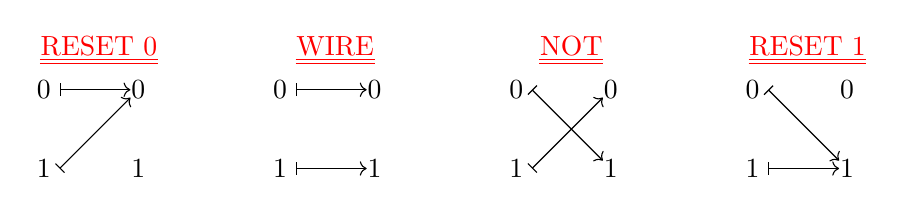
\begin{tikzpicture}
            \draw (0, 1) [|->] -- (0.9, 1);
            \draw (0, 0) [|->] -- (0.9, 0.9);
            \node at (-0.2, 1) {0};
            \node at (-0.2, 0) {1};
            \node at (1, 1) {0};
            \node at (1, 0) {1};
            \node at (0.5, 1.5) {\textcolor{red}{\uuline{RESET 0}}};

            \draw (3, 1) [|->] -- (3.9, 1);
            \draw (3, 0) [|->] -- (3.9, 0);
            \node at (2.8, 1) {0};
            \node at (2.8, 0) {1};
            \node at (4, 1) {0};
            \node at (4, 0) {1};
            \node at (3.5, 1.5) {\textcolor{red}{\uuline{WIRE}}};

            \draw (6, 1) [|->] -- (6.9, 0.1);
            \draw (6, 0) [|->] -- (6.9, 0.9);
            \node at (5.8, 1) {0};
            \node at (5.8, 0) {1};
            \node at (7, 1) {0};
            \node at (7, 0) {1};
            \node at (6.5, 1.5) {\textcolor{red}{\uuline{NOT}}};

            \draw (9, 1) [|->] -- (9.9, 0.1);
            \draw (9, 0) [|->] -- (9.9, 0);
            \node at (8.8, 1) {0};
            \node at (8.8, 0) {1};
            \node at (10, 1) {0};
            \node at (10, 0) {1};
            \node at (9.5, 1.5) {\textcolor{red}{\uuline{RESET 1}}};
        \end{tikzpicture}
    \end{center}
    One can feed an input bit \( x \in \{0, 1\} \) to the black box and ask the black box to provide $f(x)$ as the output, but cannot "look inside" and see how the black box computes the output.
    \begin{center}
        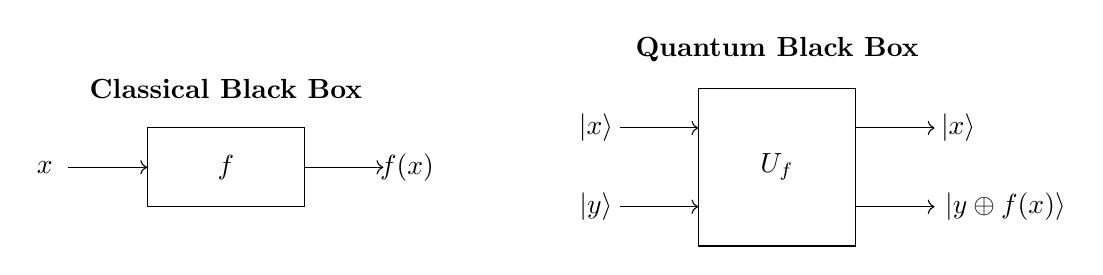
\begin{tikzpicture}
            \draw (0, 0.5) rectangle (2, 1.5) node[midway] {$f$};
            \draw[->] (-1, 1) -- (0, 1);
            \node at (-1.3, 1) {$x$};
            \draw[->] (2, 1) -- (3, 1);
            \node at (3.3, 1) {$f(x)$};
            \node at (1, 2) {\textbf{Classical Black Box}};

            \draw (7, 0) rectangle (9, 2) node[midway] {$U_f$};
            \draw[->] (6, 1.5) -- (7, 1.5);
            \node at (5.7, 1.5) {$\ket{x}$};
            \draw[->] (9, 1.5) -- (10, 1.5);
            \node at (10.3, 1.5) {$\ket{x}$};

            \draw [->] (6, 0.5) -- (7, 0.5);
            \node at (5.7, 0.5) {$\ket{y}$};
            \draw [->] (9, 0.5) -- (10, 0.5);
            \node at (10.9, 0.5) {$\ket{y \oplus f(x)}$};
            \node at (8, 2.5) {\textbf{Quantum Black Box}};
        \end{tikzpicture}
    \end{center}
    The goal is to determine if the function is balanced or constant:
    \begin{itemize}
        \item If \textcolor{blue}{$f(0) = f(1)$ or $f(0) \oplus f(1) = 0$}, then the function is \hl{constant}.
        \item If \textcolor{blue}{$f(0) \neq f(1)$ or $f(0) \oplus f(1) = 1$}, then the function is \hl{balanced}.
    \end{itemize}
\end{thmBox}
In the classical world, we need to ask the black box twice to get one bit of information $f(0) \oplus f(1)$, but in the quantum world, we only need to ask the black box once to get the same information.\\
\vspace{1mm}
Here are some examples of Deutsch's Algorithm:
\begin{enumerate}
    \item For \(\ket{\psi_1} = \frac{1}{\sqrt{2}}(\ket{x, 0} + \ket{x, 1})\), the output is \(\ket{\psi_2} = \frac{1}{\sqrt{2}}(\ket{x, f(x)} + \ket{x, f(x) \oplus 1}) = \frac{1}{\sqrt{2}}(\ket{x, 0} + \ket{x, 1})\).
    \begin{center}
        \begin{tikzpicture}
            \draw (0, 0) rectangle (3, 2) node[midway] {$U_f$};
            \draw[->] (-2, 1.5) -- (0, 1.5);
            \node at (-2.3, 1.5) {$\ket{x}$};
            \draw[->] (3, 1.5) -- (5, 1.5);
            \draw[->] (3, 0.5) -- (5, 0.5);
            \node at (-2.3, 0.5) {$\ket{0}$};
            \draw[->] (-2, 0.5) -- (-1.5, 0.5);
            \draw (-1.5, 1) rectangle (-0.5, 0) node[midway] {$H$};
            \draw[->] (-0.5, 0.5) -- (0, 0.5);
            \draw[-, red, dashed] (-0.3, -0.5) -- (-0.3, 2);
            \draw[-, red, dashed] (4, -0.5) -- (4, 2);
            \node at (-0.3, -1) {\textcolor{red}{$\ket{\psi_1} = \frac{1}{\sqrt{2}}(\ket{x, 0} + \ket{x, 1})$}};
            \node at (6, 2.5) {\textcolor{red}{$\ket{\psi_2} = \frac{1}{\sqrt{2}}(\ket{x, f(x)} + \ket{x, f(x) \oplus 1}) = \frac{1}{\sqrt{2}}(\ket{x, 0} + \ket{x, 1})$}};
        \end{tikzpicture}
    \end{center}
    \newpage
    \item For \(\ket{\psi_1} = \frac{1}{\sqrt{2}}(\ket{x, 0} - \ket{x, 1})\), the output is \(\ket{\psi_2} = \frac{1}{\sqrt{2}}(\ket{x, f(x)} - \ket{x, f(x) \oplus 1}) = \frac{\textcolor{red}{(-1)^{f(x)}}}{\sqrt{2}}\ket{x}(\ket{0} - \ket{1})\)\\
    \hfill where \textcolor{blue}{\((-1)^{f(x)} = 1\)} if \(f(x) = 0\) and \textcolor{blue}{\((-1)^{f(x)} = -1\)} if \(f(x) = 1\).
    \begin{center}
        \begin{tikzpicture}
            \draw (0, 0) rectangle (3, 2) node[midway] {$U_f$};
            \draw[->] (-2, 1.5) -- (0, 1.5);
            \node at (-2.3, 1.5) {$\ket{x}$};
            \draw[->] (3, 1.5) -- (5, 1.5);
            \draw[->] (3, 0.5) -- (5, 0.5);
            \node at (-2.3, 0.5) {\textcolor{blue}{$\ket{1}$}};
            \draw[->] (-2, 0.5) -- (-1.5, 0.5);
            \draw (-1.5, 1) rectangle (-0.5, 0) node[midway] {$H$};
            \draw[->] (-0.5, 0.5) -- (0, 0.5);
            \draw[-, orange, dashed] (-0.3, -0.5) -- (-0.3, 2);
            \draw[-, orange, dashed] (4, -0.5) -- (4, 2);
            \node at (-0.3, -1) {\textcolor{orange}{$\ket{\psi_1} = \frac{1}{\sqrt{2}}(\ket{x, 0} - \ket{x, 1})$}};
            \node at (6, 2.5) {\textcolor{orange}{$\ket{\psi_2} = \frac{1}{\sqrt{2}}(\ket{x, f(x)} - \ket{x, f(x) \oplus 1}) = \frac{\textcolor{red}{(-1)^{f(x)}}}{\sqrt{2}}\ket{x}(\ket{0} - \ket{1})$}};
        \end{tikzpicture}
    \end{center}
    \item For \(\ket{\psi_1} = \frac{1}{2}(\ket{0} + \ket{1})(\ket{0} - \ket{1})\),\\
    the outputs are \(\ket{\psi_2} = \frac{1}{2}((-1)^{f(0)}\ket{0} + (-1)^{f(1)}\ket{1})(\ket{0} - \ket{1})\) and \(\ket{\psi_3} = \frac{1}{\sqrt{2}}(\ket{f(0) \oplus f(1)})(\ket{0} - \ket{1})\).
    \vspace{1mm}
    \fbox{
        \parbox{0.94\textwidth}{  
    \textit{\textbf{Remark:}} The measurement of the first qubit always outputs $\ket{0} \oplus \ket{1}$, but the measurement of the second qubit will determine if the function is constant or balanced.}}
    \begin{center}
        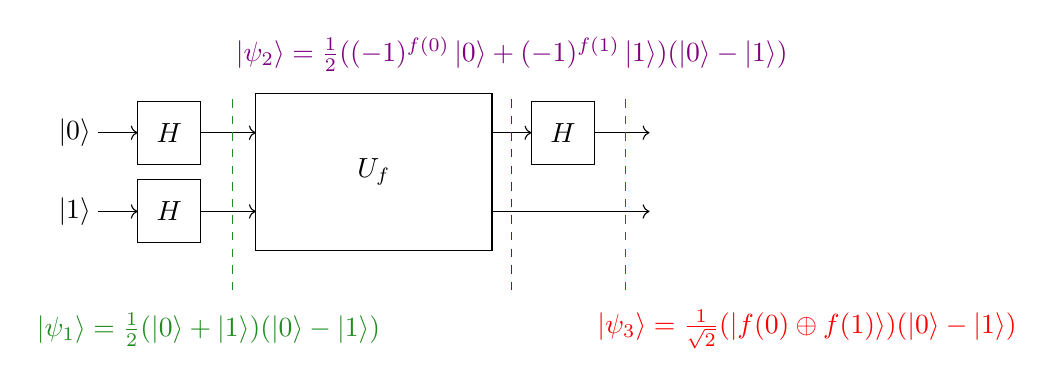
\begin{tikzpicture}
            \draw (0, 0) rectangle (3, 2) node[midway] {$U_f$};
            \draw[->] (-2, 1.5) -- (-1.5, 1.5);
            \draw (-1.5, 1.9) rectangle (-0.7, 1.1) node[midway] {$H$};
            \draw[->] (-0.7, 1.5) -- (0, 1.5);
            \node at (-2.3, 1.5) {$\ket{0}$};
            \draw[->] (3, 1.5) -- (3.5, 1.5);
            \draw (3.5, 1.9) rectangle (4.3, 1.1) node[midway] {$H$};
            \draw[->] (4.3, 1.5) -- (5, 1.5);
            \draw[->] (3, 0.5) -- (5, 0.5);
            \node at (-2.3, 0.5) {$\ket{1}$};
            \draw[->] (-2, 0.5) -- (-1.5, 0.5);
            \draw (-1.5, 0.9) rectangle (-0.7, 0.1) node[midway] {$H$};
            \draw[->] (-0.7, 0.5) -- (0, 0.5);
            \draw[-, forestgreen, dashed] (-0.3, -0.5) -- (-0.3, 2);
            \draw[-, violet, dashed] (3.25, -0.5) -- (3.25, 2);
            \draw[-, red, dashed] (4.7, -0.5) -- (4.7, 2);
            \node at (-0.6, -1) {\textcolor{forestgreen}{$\ket{\psi_1} = \frac{1}{2}(\ket{0} + \ket{1})(\ket{0} - \ket{1})$}};
            \node at (3.25, 2.5) {\textcolor{violet}{$\ket{\psi_2} = \frac{1}{2}((-1)^{f(0)}\ket{0} + (-1)^{f(1)}\ket{1})(\ket{0} - \ket{1})$}};
            \node at (7, -1) {\textcolor{red}{$\ket{\psi_3} = \frac{1}{\sqrt{2}}(\ket{f(0) \oplus f(1)})(\ket{0} - \ket{1})$}};
        \end{tikzpicture}
    \end{center}
    There are two cases for the outputs: \hl{$f(0) = f(1)$} and \hl{$f(0) \neq f(1)$}.\\
    \uwave{Case 1:} If \textcolor{blue}{\(f(0) = f(1)\)}, then \(\ket{\psi_2} = \frac{(-1)^{f(0)}}{2}(\ket{0} + \ket{1})(\ket{0} - \ket{1})\) and \(\ket{\psi_3} = \frac{(-1)^{f(0)}}{\textcolor{orange}{\sqrt{2}}}\textcolor{orange}{\ket{0}}(\ket{0} - \ket{1})\).\\
    \begin{center}
        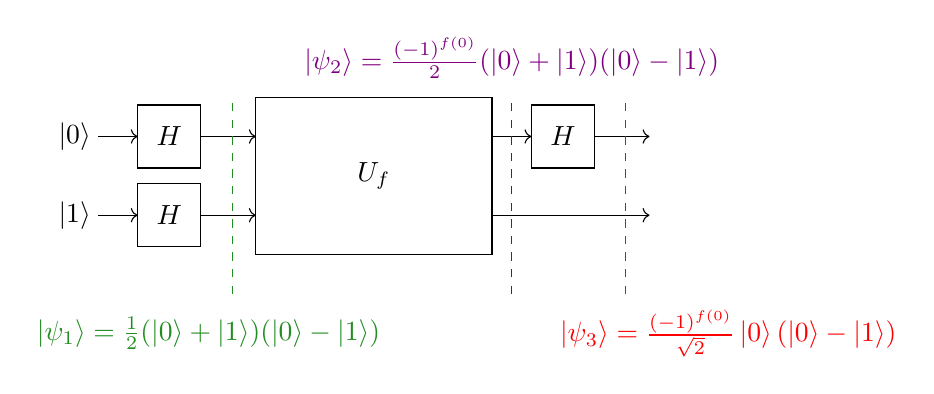
\begin{tikzpicture}
            \draw (0, 0) rectangle (3, 2) node[midway] {$U_f$};
            \draw[->] (-2, 1.5) -- (-1.5, 1.5);
            \draw (-1.5, 1.9) rectangle (-0.7, 1.1) node[midway] {$H$};
            \draw[->] (-0.7, 1.5) -- (0, 1.5);
            \node at (-2.3, 1.5) {$\ket{0}$};
            \draw[->] (3, 1.5) -- (3.5, 1.5);
            \draw (3.5, 1.9) rectangle (4.3, 1.1) node[midway] {$H$};
            \draw[->] (4.3, 1.5) -- (5, 1.5);
            \draw[->] (3, 0.5) -- (5, 0.5);
            \node at (-2.3, 0.5) {$\ket{1}$};
            \draw[->] (-2, 0.5) -- (-1.5, 0.5);
            \draw (-1.5, 0.9) rectangle (-0.7, 0.1) node[midway] {$H$};
            \draw[->] (-0.7, 0.5) -- (0, 0.5);
            \draw[-, forestgreen, dashed] (-0.3, -0.5) -- (-0.3, 2);
            \draw[-, violet, dashed] (3.25, -0.5) -- (3.25, 2);
            \draw[-, red, dashed] (4.7, -0.5) -- (4.7, 2);
            \node at (-0.6, -1) {\textcolor{forestgreen}{$\ket{\psi_1} = \frac{1}{2}(\ket{0} + \ket{1})(\ket{0} - \ket{1})$}};
            \node at (3.25, 2.5) {\textcolor{violet}{$\ket{\psi_2} = \frac{(-1)^{f(0)}}{2}(\ket{0} + \ket{1})(\ket{0} - \ket{1})$}};
            \node at (6, -1) {\textcolor{red}{$\ket{\psi_3} = \frac{(-1)^{f(0)}}{\sqrt{2}}\ket{0}(\ket{0} - \ket{1})$}};
        \end{tikzpicture}
    \end{center}
    \uwave{Case 2:} If \textcolor{blue}{\(f(0) \neq f(1)\)}, then \(\ket{\psi_2} = \frac{(-1)^{f(0)}}{2}(\ket{0} - \ket{1})(\ket{0} - \ket{1})\) and \(\ket{\psi_3} = \frac{(-1)^{f(0)}}{\textcolor{orange}{\sqrt{2}}}\textcolor{orange}{\ket{1}}(\ket{0} - \ket{1})\).\\
    \begin{center}
        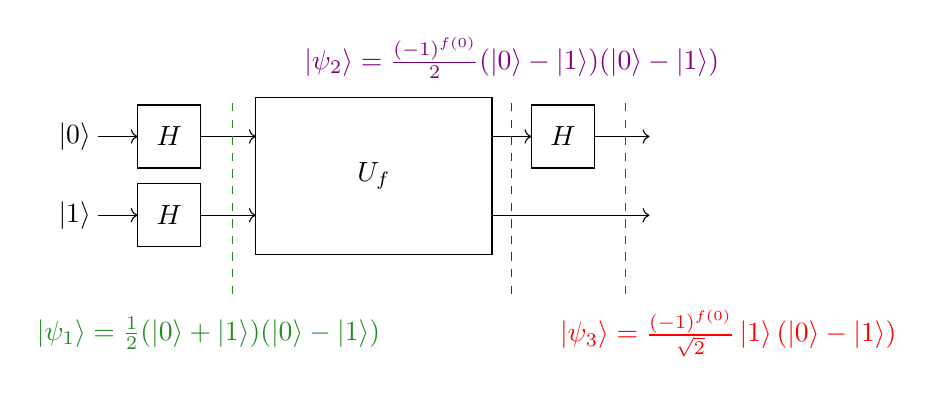
\begin{tikzpicture}
            \draw (0, 0) rectangle (3, 2) node[midway] {$U_f$};
            \draw[->] (-2, 1.5) -- (-1.5, 1.5);
            \draw (-1.5, 1.9) rectangle (-0.7, 1.1) node[midway] {$H$};
            \draw[->] (-0.7, 1.5) -- (0, 1.5);
            \node at (-2.3, 1.5) {$\ket{0}$};
            \draw[->] (3, 1.5) -- (3.5, 1.5);
            \draw (3.5, 1.9) rectangle (4.3, 1.1) node[midway] {$H$};
            \draw[->] (4.3, 1.5) -- (5, 1.5);
            \draw[->] (3, 0.5) -- (5, 0.5);
            \node at (-2.3, 0.5) {$\ket{1}$};
            \draw[->] (-2, 0.5) -- (-1.5, 0.5);
            \draw (-1.5, 0.9) rectangle (-0.7, 0.1) node[midway] {$H$};
            \draw[->] (-0.7, 0.5) -- (0, 0.5);
            \draw[-, forestgreen, dashed] (-0.3, -0.5) -- (-0.3, 2);
            \draw[-, violet, dashed] (3.25, -0.5) -- (3.25, 2);
            \draw[-, red, dashed] (4.7, -0.5) -- (4.7, 2);
            \node at (-0.6, -1) {\textcolor{forestgreen}{$\ket{\psi_1} = \frac{1}{2}(\ket{0} + \ket{1})(\ket{0} - \ket{1})$}};
            \node at (3.25, 2.5) {\textcolor{violet}{$\ket{\psi_2} = \frac{(-1)^{f(0)}}{2}(\ket{0} - \ket{1})(\ket{0} - \ket{1})$}};
            \node at (6, -1) {\textcolor{red}{$\ket{\psi_3} = \frac{(-1)^{f(0)}}{\sqrt{2}}\ket{1}(\ket{0} - \ket{1})$}};
        \end{tikzpicture}
    \end{center}
    \newpage
    \item For \(\ket{\psi_1} = \frac{1}{2}(\ket{0} + \ket{1})(\ket{0} - \ket{1})\), \\
    the output is \(\ket{\psi_2} = \frac{1}{2}((-1)^{f(0)}\ket{0} + (-1)^{f(1)}\ket{1})(\ket{0} - \ket{1}) = \frac{(-1)^{f(0)}}{2}(\ket{0} + (-1)^{f(0) \oplus f(1)}\ket{1})(\ket{0} - \ket{1})\).
    \begin{center}
        \begin{tikzpicture}
            \draw (0, 0) rectangle (3, 2) node[midway] {$U_f$};
            \draw[->] (-2, 1.5) -- (-1.5, 1.5);
            \draw (-1.5, 1.9) rectangle (-0.7, 1.1) node[midway] {$H$};
            \draw[->] (-0.7, 1.5) -- (0, 1.5);
            \node at (-2.3, 1.5) {$\ket{0}$};
            \draw[->] (3, 1.5) -- (5, 1.5);
            \draw[->] (3, 0.5) -- (5, 0.5);
            \node at (-2.3, 0.5) {$\ket{1}$};
            \draw[->] (-2, 0.5) -- (-1.5, 0.5);
            \draw (-1.5, 0.9) rectangle (-0.7, 0.1) node[midway] {$H$};
            \draw[->] (-0.7, 0.5) -- (0, 0.5);
            \draw[-, violet, dashed] (-0.3, -0.5) -- (-0.3, 2);
            \draw[-, violet, dashed] (4, -0.5) -- (4, 2);
            \node at (-0.3, -1) {\textcolor{violet}{$\ket{\psi_1} = \frac{1}{2}(\ket{0} + \ket{1})(\ket{0} - \ket{1})$}};
            \node at (8, 2.5) {\textcolor{violet}{$\ket{\psi_2} = \frac{1}{2}((-1)^{f(0)}\ket{0} + (-1)^{f(1)}\ket{1})(\ket{0} - \ket{1}) = \frac{(-1)^{f(0)}}{2}(\ket{0} + (-1)^{f(0) \oplus f(1)}\ket{1})(\ket{0} - \ket{1})$}};
        \end{tikzpicture}
    \end{center}
\end{enumerate}



\chapter{Matrix Representation of Quantum Gates and Circuits}
\textcolor{magenta}{\section{\textbf{Matrix Representation of Single-Qubit States and Gates}}}
\subsection{Matrix Representation and Multiplication}
\textcolor{purple}{\textbf{$2 \times 1$ array representation of a single-qubit state $\ket{\psi} = \alpha\ket{0} + \beta\ket{1}$:}}
\[
    \boxed{\textcolor{teal}{\text{VEC}(\ket{\alpha\ket{0} + \beta\ket{1}}) = \begin{bmatrix} \alpha \\ \beta \end{bmatrix}}}
\]
\fbox{
    \parbox{0.97\textwidth}{
\textit{\textbf{Remark:}} We cannot write $\ket{0} = \begin{bmatrix} 0 \\ 1 \end{bmatrix}$ and $\ket{1} = \begin{bmatrix} 1 \\ 0 \end{bmatrix}$ as it will lose the linearity of quantum mechanics.}}\\
\vspace{2mm}
$\implies$ Vector Addition of $2 \times 1$ arrays of single-qubit states:
\[
    \boxed{\textcolor{teal}{\text{VEC}(\alpha\ket{0} + \beta\ket{1}) + \text{VEC}(\gamma\ket{0} + \delta\ket{1}) = \begin{bmatrix} \alpha \\ \beta \end{bmatrix} + \begin{bmatrix} \gamma \\ \delta \end{bmatrix} = \begin{bmatrix} \alpha + \gamma \\ \beta + \delta \end{bmatrix}}}
\]
$\implies$ Scalar Multiplication of $2 \times 1$ arrays of single-qubit states:
\[
    \boxed{\textcolor{teal}{c(\text{VEC}(\alpha\ket{0} + \beta\ket{1})) = c \begin{bmatrix} \alpha \\ \beta \end{bmatrix} = \begin{bmatrix} c\alpha \\ c\beta \end{bmatrix}}} 
\]
\textcolor{purple}{\textbf{$2 \times 2$ matrix representation of single-qubit gates:}}\\
\textcolor{blue}{\textbf{U Gate:}} $\begin{cases}
    U\ket{0} = \textcolor{forestgreen}{u_{00}}\ket{0} + \textcolor{forestgreen}{u_{10}}\ket{1} \\
    U\ket{1} = \textcolor{forestgreen}{u_{01}}\ket{0} + \textcolor{forestgreen}{u_{11}}\ket{1}
\end{cases}$ \\
\hspace{1.5cm} $\implies 2\times 2$ Matrix representation of the U gate: $\boxed{\textcolor{red}{U = \begin{bmatrix} u_{00} & u_{01} \\ u_{10} & u_{11} \end{bmatrix}}}
$ \\
\textcolor{blue}{\textbf{X Gate:}} $\begin{cases}
    X\ket{0} = \ket{1} = \textcolor{forestgreen}{0}\ket{0} + \textcolor{forestgreen}{1}\ket{1} \\
    X\ket{1} = \ket{0} = \textcolor{forestgreen}{1}\ket{0} + \textcolor{forestgreen}{0}\ket{1}
\end{cases}$\\
\hspace{1.5cm} $\implies 2\times 2$ Matrix representation of the X gate: $\boxed{\textcolor{red}{X = \begin{bmatrix} 0 & 1 \\ 1 & 0 \end{bmatrix}}}$\\
\textcolor{blue}{\textbf{Z Gate:}} $\begin{cases}
    Z\ket{0} = \ket{0} = \textcolor{forestgreen}{1}\ket{0} + \textcolor{forestgreen}{0}\ket{1} \\
    Z\ket{1} = -\ket{1} = \textcolor{forestgreen}{0}\ket{0} - \textcolor{forestgreen}{1}\ket{1}
\end{cases}$ \\
\hspace{1.5cm} $\implies 2\times 2$ Matrix representation of the Z gate: $\boxed{\textcolor{red}{Z = \begin{bmatrix} 1 & 0 \\ 0 & -1 \end{bmatrix}}}$\\
\textcolor{blue}{\textbf{Hadamard Gate:}} $\begin{cases}
    H\ket{0} = \frac{1}{\sqrt{2}}(\ket{0} + \ket{1}) = \textcolor{forestgreen}{\frac{1}{\sqrt{2}}}\ket{0} + \textcolor{forestgreen}{\frac{1}{\sqrt{2}}}\ket{1} \\
    H\ket{1} = \frac{1}{\sqrt{2}}(\ket{0} - \ket{1}) = \textcolor{forestgreen}{\frac{1}{\sqrt{2}}}\ket{0} - \textcolor{forestgreen}{\frac{1}{\sqrt{2}}}\ket{1}
\end{cases}$ \\
\hspace{3cm} $\implies 2\times 2$ Matrix representation of the H gate: $\boxed{\textcolor{red}{H = \begin{bmatrix}
        \frac{1}{\sqrt{2}} & \frac{1}{\sqrt{2}} \\
        \frac{1}{\sqrt{2}} & -\frac{1}{\sqrt{2}}
    \end{bmatrix} = \frac{1}{\sqrt{2}}\begin{bmatrix}
        1 & 1 \\
        1 & -1
    \end{bmatrix}}} $
\newpage
\textcolor{purple}{\textbf{Transformation of State Vectors by Quantum Gates:}}\\
\textcolor{blue}{\textbf{U Gate}}: \( U(\alpha \ket{0} + \beta \ket{1}) = \alpha U\ket{0} + \beta U\ket{1} = \alpha(u_{00}\ket{0} + u_{10}\ket{1}) + \beta(u_{01}\ket{0} + u_{11}\ket{1}) = (u_{00}\alpha + u_{01}\beta)\ket{0} + (u_{10}\alpha + u_{11}\beta)\ket{1} \)\\
\hspace{1.5cm} $\implies$ Transformation of state vectors by the U gate: $\boxed{\textcolor{red}{\begin{bmatrix} u_{00} & u_{01} \\ u_{10} & u_{11} \end{bmatrix} \begin{bmatrix} \alpha \\ \beta \end{bmatrix} = \begin{bmatrix} u_{00}\alpha + u_{01}\beta \\ u_{10}\alpha + u_{11}\beta \end{bmatrix}}}$\\
\vspace{2mm}
\textcolor{blue}{\textbf{X Gate}}: \( X(\alpha \ket{0} + \beta \ket{1}) = \alpha X\ket{0} + \beta X\ket{1} = \alpha\ket{1} + \beta\ket{0} = \beta\ket{0} + \alpha\ket{1} \)\\
\hspace{1.5cm} $\implies$ Transformation of state vectors by the X gate: $\boxed{\textcolor{red}{\begin{bmatrix} 0 & 1 \\ 1 & 0 \end{bmatrix} \begin{bmatrix} \alpha \\ \beta \end{bmatrix} = \begin{bmatrix} \beta \\ \alpha \end{bmatrix}}}$\\
\vspace{2mm}
\textcolor{blue}{\textbf{Z Gate}}: \( Z(\alpha \ket{0} + \beta \ket{1}) = \alpha Z\ket{0} + \beta Z\ket{1} = \alpha\ket{0} - \beta\ket{1} \)\\
\hspace{1.5cm} $\implies$ Transformation of state vectors by the Z gate: $\boxed{\textcolor{red}{\begin{bmatrix} 1 & 0 \\ 0 & -1 \end{bmatrix} \begin{bmatrix} \alpha \\ \beta \end{bmatrix} = \begin{bmatrix} \alpha \\ -\beta \end{bmatrix}}}$\\
\vspace{2mm}
\textcolor{blue}{\textbf{Hadamard Gate}}: \( H(\alpha \ket{0} + \beta \ket{1}) = \alpha H\ket{0} + \beta H\ket{1} = \alpha\frac{1}{\sqrt{2}}(\ket{0} + \ket{1}) + \beta\frac{1}{\sqrt{2}}(\ket{0} - \ket{1}) = \frac{1}{\sqrt{2}}(\alpha + \beta)\ket{0} + \frac{1}{\sqrt{2}}(\alpha - \beta)\ket{1} \)\\
\hspace{3cm} $\implies$ Transformation of state vectors by the H gate: $\boxed{\textcolor{red}{\begin{bmatrix} \frac{1}{\sqrt{2}} & \frac{1}{\sqrt{2}} \\ \frac{1}{\sqrt{2}} & -\frac{1}{\sqrt{2}} \end{bmatrix} \begin{bmatrix} \alpha \\ \beta \end{bmatrix} = \begin{bmatrix} \frac{1}{\sqrt{2}}(\alpha + \beta) \\ \frac{1}{\sqrt{2}}(\alpha - \beta) \end{bmatrix}}}$\\
\subsection{Seqeuntial Gates}
\begin{defBox}{Definition 3.1}{Seqeuntial Gates}
    \raggedright
    \textcolor{cyan}{\textbf{Sequential Gates:}} If we apply two gates $A$ and $B$ in sequence, then the matrix representation of the combined gate is the \\
    \hspace{3.2cm} matrix product of the individual gates, read from \textcolor{red}{right to left}.
    \begin{center}
        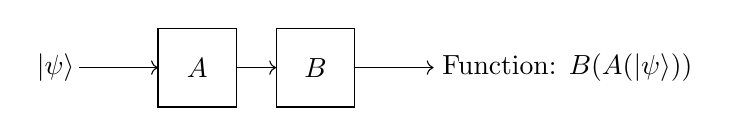
\begin{tikzpicture}
            \draw (0, 0) rectangle (1, 1) node[midway] {$A$};
            \draw (1.5, 0) rectangle (2.5, 1) node[midway] {$B$};
            \draw[->] (-1, 0.5) -- (0, 0.5);
            \draw[->] (1, 0.5) -- (1.5, 0.5);
            \node at (-1.3, 0.5) {$\ket{\psi}$};
            \draw[->] (2.5, 0.5) -- (3.5, 0.5);
            \node at (5.2, 0.5) {Function: $B(A(\ket{\psi}))$};
        \end{tikzpicture}
    \end{center}
    $\implies$ Matrix representation is \hl{$\text{MAT}(B) \cdot \text{MAT}(A) \cdot \text{VEC}(\ket{\psi}) = B(A(\ket{\psi}))$}.
\end{defBox}
\begin{egBox}{Example 3.1}{Difference between $XH$ and $HX$ Circuits}
    \begin{center}
        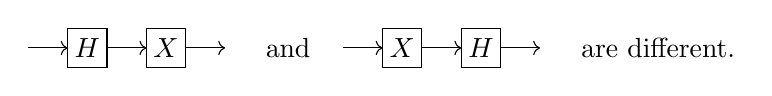
\begin{tikzpicture}
            \draw(0, 0) rectangle(0.5, 0.5) node[midway] {$H$};
            \draw(1, 0) rectangle(1.5, 0.5) node[midway] {$X$};
            \draw[->] (-0.5, 0.25) -- (0, 0.25);
            \draw[->] (0.5, 0.25) -- (1, 0.25);
            \draw[->] (1.5, 0.25) -- (2, 0.25);

            \node at (2.8, 0.25) {and};

            \draw(4, 0) rectangle(4.5, 0.5) node[midway] {$X$};
            \draw(5, 0) rectangle(5.5, 0.5) node[midway] {$H$};
            \draw[->] (3.5, 0.25) -- (4, 0.25);
            \draw[->] (4.5, 0.25) -- (5, 0.25);
            \draw[->] (5.5, 0.25) -- (6, 0.25);
            \node at (7.5, 0.25) {are different.};
        \end{tikzpicture}
    \end{center}
    \begin{align*}
        XH &= \begin{bmatrix} 0 & 1 \\ 1 & 0 \end{bmatrix} \cdot \frac{1}{\sqrt{2}}\begin{bmatrix} 1 & 1 \\ 1 & -1 \end{bmatrix} = \frac{1}{\sqrt{2}}\begin{bmatrix} 1 & -1 \\ 1 & 1 \end{bmatrix} \\
        HX &= \frac{1}{\sqrt{2}}\begin{bmatrix} 1 & 1 \\ 1 & -1 \end{bmatrix} \cdot \begin{bmatrix} 0 & 1 \\ 1 & 0 \end{bmatrix} = \frac{1}{\sqrt{2}}\begin{bmatrix} 1 & 1 \\ -1 & 1 \end{bmatrix} \neq XH 
    \end{align*}
\end{egBox}
\textcolor{purple}{\textbf{Useful Identities for Single-Qubit Gates:}}
\begin{enumerate}
    \item \textcolor{blue}{$HZH = X$}: \(\frac{1}{\sqrt{2}} \begin{bmatrix} 1 & 1 \\ 1 & -1 \end{bmatrix} \cdot \begin{bmatrix} 1 & 0 \\ 0 & -1 \end{bmatrix} \cdot \frac{1}{\sqrt{2}} \begin{bmatrix} 1 & 1 \\ 1 & -1 \end{bmatrix} = \begin{bmatrix} 0 & 1 \\ 1 & 0 \end{bmatrix}\).
    \item \textcolor{blue}{$HXH = Z$}: \(\begin{bmatrix} 0 & 1 \\ 1 & 0 \end{bmatrix} \cdot \frac{1}{\sqrt{2}} \begin{bmatrix} 1 & 1 \\ 1 & -1 \end{bmatrix} \cdot \begin{bmatrix} 0 & 1 \\ 1 & 0 \end{bmatrix} = \begin{bmatrix} 1 & 0 \\ 0 & -1 \end{bmatrix}\).
\end{enumerate}
\textcolor{magenta}{\section{\textbf{Matrix Representation of Multi-Qubit States and Gates}}}
\subsection{Matrix Representation of Two-Qubit States and Gates}
\textcolor{purple}{\textbf{$4 \times 1$ array representation of two-qubit states:}}\\
$\implies$ The two-qubit state $\ket{\psi} = a_{00}\ket{00} + a_{01}\ket{01} + a_{10}\ket{10} + a_{11}\ket{11}$ is represented as:
\[
    \boxed{\textcolor{teal}{\text{VEC}(\ket{\psi}) = a_{00}\begin{bmatrix} 1 \\ 0 \\ 0 \\ 0 \end{bmatrix} + a_{01}\begin{bmatrix} 0 \\ 1 \\ 0 \\ 0 \end{bmatrix} + a_{10}\begin{bmatrix} 0 \\ 0 \\ 1 \\ 0 \end{bmatrix} + a_{11}\begin{bmatrix} 0 \\ 0 \\ 0 \\ 1 \end{bmatrix} = \begin{bmatrix} a_{00} \\ a_{01} \\ a_{10} \\ a_{11} \end{bmatrix}}}
\]
\newpage
\textcolor{purple}{\textbf{CNOT Gate $4 \times 4$ Matrix Representation:}}\\
\begin{itemize}
    \item $\ket{x, y}$ is the input state and $\ket{x, y \oplus x}$ is the output state (First qubit is the control qubit).
    \[
        \begin{blockarray}
        {cccccc}
        \textcolor{red}{\text{Output}} & \textcolor{cyan}{\ket{00}} & \textcolor{cyan}{\ket{01}} & \textcolor{cyan}{\ket{10}} & \textcolor{cyan}{\ket{11}} & \textcolor{cyan}{\text{Input}} \\
        \begin{block}{c[cccc]c}
        \textcolor{red}{\ket{00}} & 1 & 0 & 0 & 0 & \\
        \textcolor{red}{\ket{01}} & 0 & 1 & 0 & 0 & \\
        \textcolor{red}{\ket{10}} & 0 & 0 & 0 & 1 & \\
        \textcolor{red}{\ket{11}} & 0 & 0 & 1 & 0 & \\
        \end{block}
        \end{blockarray}
    \]
    \item $\ket{x, y}$ is the input state and $\ket{x \oplus y, y}$ is the output state (Second qubit is the control qubit).
    \[
        \begin{blockarray}
        {cccccc}
        \textcolor{red}{\text{Output}} & \textcolor{cyan}{\ket{00}} & \textcolor{cyan}{\ket{01}} & \textcolor{cyan}{\ket{10}} & \textcolor{cyan}{\ket{11}} & \textcolor{cyan}{\text{Input}} \\
        \begin{block}{c[cccc]c}
        \textcolor{red}{\ket{00}} & 1 & 0 & 0 & 0 & \\
        \textcolor{red}{\ket{01}} & 0 & 0 & 0 & 1 & \\
        \textcolor{red}{\ket{10}} & 0 & 0 & 1 & 0 & \\
        \textcolor{red}{\ket{11}} & 0 & 1 & 0 & 0 & \\
        \end{block}
        \end{blockarray}
    \]
\end{itemize}

\textcolor{purple}{\textbf{Controlled-Z Gate $4 \times 4$ Matrix Representation:}}\\
\begin{itemize}
    \item Given $\ket{00} \rightarrow \ket{00}$, $\ket{01} \rightarrow \ket{01}$, $\ket{10} \rightarrow \ket{10}$, $\ket{11} \rightarrow -\ket{11}$, the matrix representation is:
    \begin{center}
        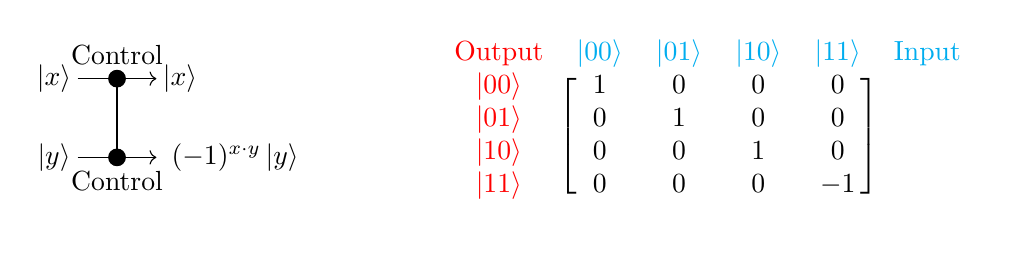
\begin{tikzpicture}
        \draw [->] (0, 0) -- (1, 0);
        \draw [->] (0, -1) -- (1, -1);
        \draw [-] (0.5, 0) -- (0.5, -1);
        \node at (0.5, -1.3) {Control};
        \node at (0.5, 0.3) {Control};
        \filldraw[fill=black, draw=black] (0.5, 0) circle (3pt);
        \filldraw[fill=black, draw=black] (0.5, -1) circle (3pt);
        \node at (-0.3, 0) {$\ket{x}$};
        \node at (-0.3, -1) {$\ket{y}$};
        \node at (1.3, 0) {$\ket{x}$};
        \node at (2, -1) {$(-1)^{x \cdot y}\ket{y}$};

        \node at (8, -0.7) {$\begin{blockarray}
        {cccccc}
        \textcolor{red}{\text{Output}} & \textcolor{cyan}{\ket{00}} & \textcolor{cyan}{\ket{01}} & \textcolor{cyan}{\ket{10}} & \textcolor{cyan}{\ket{11}} & \textcolor{cyan}{\text{Input}} \\
        \begin{block}{c[cccc]c}
        \textcolor{red}{\ket{00}} & 1 & 0 & 0 & 0 & \\
        \textcolor{red}{\ket{01}} & 0 & 1 & 0 & 0 & \\
        \textcolor{red}{\ket{10}} & 0 & 0 & 1 & 0 & \\
        \textcolor{red}{\ket{11}} & 0 & 0 & 0 & -1 & \\
        \end{block}
        \end{blockarray}$};
        \end{tikzpicture}
    \end{center}
\end{itemize}
\subsection{Matrix Representation of 3-Qubit States and Gates}
\textcolor{purple}{\textbf{$8 \times 1$ array representation of 3-qubit states:}}\\
$\implies$ The 8 states of a 3-qubit system are $\ket{000}$, $\ket{001}$, $\ket{010}$, $\ket{011}$, $\ket{100}$, $\ket{101}$, $\ket{110}$, and $\ket{111}$.\\
\begin{align*}
    & \ket{000} \leftrightarrow \begin{bmatrix} 1 \\ 0 \\ 0 \\ 0 \\ 0 \\ 0 \\ 0 \\ 0 \end{bmatrix}, \quad \ket{001} \leftrightarrow \begin{bmatrix} 0 \\ 1 \\ 0 \\ 0 \\ 0 \\ 0 \\ 0 \\ 0 \end{bmatrix}, \quad \ket{010} \leftrightarrow \begin{bmatrix} 0 \\ 0 \\ 1 \\ 0 \\ 0 \\ 0 \\ 0 \\ 0 \end{bmatrix}, \quad \ket{011} \leftrightarrow \begin{bmatrix} 0 \\ 0 \\ 0 \\ 1 \\ 0 \\ 0 \\ 0 \\ 0 \end{bmatrix}, \quad \ket{100} \leftrightarrow \begin{bmatrix} 0 \\ 0 \\ 0 \\ 0 \\ 1 \\ 0 \\ 0 \\ 0 \end{bmatrix}, \quad \ket{101} \leftrightarrow \begin{bmatrix} 0 \\ 0 \\ 0 \\ 0 \\ 0 \\ 1 \\ 0 \\ 0 \end{bmatrix}, \quad \ket{110} \leftrightarrow \begin{bmatrix} 0 \\ 0 \\ 0 \\ 0 \\ 0 \\ 0 \\ 1 \\ 0 \end{bmatrix}, \quad \ket{111} \leftrightarrow \begin{bmatrix} 0 \\ 0 \\ 0 \\ 0 \\ 0 \\ 0 \\ 0 \\ 1 \end{bmatrix}
\end{align*}
\textcolor{purple}{\textbf{Toffoli Gate $8 \times 8$ Matrix Representation:}}
    \[
        \begin{blockarray}
        {cccccccccc}
        \textcolor{red}{\text{Output}} & \textcolor{cyan}{\ket{000}} & \textcolor{cyan}{\ket{001}} & \textcolor{cyan}{\ket{010}} & \textcolor{cyan}{\ket{011}} & \textcolor{cyan}{\ket{100}} & \textcolor{cyan}{\ket{101}} & \textcolor{cyan}{\ket{110}} & \textcolor{cyan}{\ket{111}} & \textcolor{cyan}{\text{Input}} \\
        \begin{block}{c[cccccccc]c}
        \textcolor{red}{\ket{000}} & 1 & 0 & 0 & 0 & 0 & 0 & 0 & 0 & \\
        \textcolor{red}{\ket{001}} & 0 & 1 & 0 & 0 & 0 & 0 & 0 & 0 & \\
        \textcolor{red}{\ket{010}} & 0 & 0 & 1 & 0 & 0 & 0 & 0 & 0 & \\
        \textcolor{red}{\ket{011}} & 0 & 0 & 0 & 1 & 0 & 0 & 0 & 0 & \\
        \textcolor{red}{\ket{100}} & 0 & 0 & 0 & 0 & 1 & 0 & 0 & 0 & \\
        \textcolor{red}{\ket{101}} & 0 & 0 & 0 & 0 & 0 & 1 & 0 & 0 & \\
        \textcolor{red}{\ket{110}} & 0 & 0 & 0 & 0 & 0 & 0 & 0 & 1 & \\
        \textcolor{red}{\ket{111}} & 0 & 0 & 0 & 0 & 0 & 0 & 1 & 0 & \\
        \end{block}
        \end{blockarray}
    \]
\newpage
\subsection{Matrix Representation of n-Qubit States}
\begin{thmBox}{Theorem 3.1}{Matrix Representation of n-Qubit States}
    The $2^n \times 1$ array representation of an n-qubit state $\ket{\psi} = \sum_{x=0}^{2^n-1} a_x\ket{x}$ is given by:
    \[
        \boxed{\textcolor{teal}{\ket{a_{n-1}a_{n-2}\ldots a_1a_0} \leftrightarrow \begin{bmatrix} a_0 \\ a_1 \\ a_2 \\ \vdots \\ a_{2^n-1} \end{bmatrix}}} \quad \text{where} \quad a_x \in \{0, 1\}.
    \]
\end{thmBox}
\fbox{
    \parbox{0.97\textwidth}{
\textit{\textbf{Remark:}} The entry indices of the $2^n \times 1$ array representation of an n-qubit state begins at 0 and ends at $2^n-1$.}}\\
\textcolor{magenta}{\section{\textbf{Tensor Product of Qubit States and Gates}}}
\begin{thmBox}{Theorem 3.2}{Tensor Product of Two Matrices}
    \raggedright
    Let $A = \begin{bmatrix} a_{0,0} & \ldots & a_{0,n-1} \\ \vdots & \ddots & \vdots \\ a_{m-1,0} & \ldots & a_{m-1,n-1} \end{bmatrix}$ be a $m \times n$ matrix and $B$ be a $p \times q$ matrix.\\
    \vspace{2mm}
    $\implies$ \textcolor{red}{Tensor/Kronecker Product} of $A$ and $B$ is a $(mp) \times (nq)$ matrix given by:
    \[
        \boxed{\textcolor{teal}{A \otimes B = \begin{bmatrix} a_{0,0}B & \ldots & a_{0,n-1}B \\ \vdots & \ddots & \vdots \\ a_{m-1,0}B & \ldots & a_{m-1,n-1}B \end{bmatrix}}}
    \]
\end{thmBox}
\subsection{Tensor Product of Qubit States}
\begin{thmBox}{Theorem 3.3}{Tensor Product of 2-Qubit States}
    The \textcolor{red}{two-qubit joint state (tensor product of two-qubits)} $\ket{\psi_1} = a\ket{0} + b\ket{1}$ and $\ket{\psi_2} = c\ket{0} + d\ket{1}$ is given by:
    \[
        \boxed{\textcolor{teal}{\ket{\psi_1} \otimes \ket{\psi_2} = (a\ket{0} + b\ket{1}) \otimes (c\ket{0} + d\ket{1}) = ac\ket{00} + ad\ket{01} + bc\ket{10} + bd\ket{11}}}
    \]
    $\implies$ The $4 \times 1$ array representation of the two-qubit joint state is:
    \[
        \begin{bmatrix} a \\ b \end{bmatrix} \otimes \begin{bmatrix} c \\ d \end{bmatrix} = \begin{bmatrix} a \begin{bmatrix} c \\ d \end{bmatrix} \\ b \begin{bmatrix} c \\ d \end{bmatrix} \end{bmatrix} = \begin{blockarray}{cc}
            \begin{block}{[c]c}
                ac & \textcolor{red}{\ket{00}} \\
                ad & \textcolor{red}{\ket{01}} \\
                bc & \textcolor{red}{\ket{10}} \\
                bd & \textcolor{red}{\ket{11}} \\
            \end{block}  
        \end{blockarray}\quad \text{which is a \textcolor{orange}{separable} state}
    \]
\end{thmBox}
Examples of Tensor Product of 2-Qubit States:
\begin{itemize}
    \item \uline{\textbf{e.g. 1}}: $\ket{0} \otimes \ket{0} = \begin{bmatrix} 1 \\ 0 \end{bmatrix} \otimes \begin{bmatrix} 1 \\ 0 \end{bmatrix} = \begin{bmatrix} 1 \begin{bmatrix} 1 \\ 0 \end{bmatrix} \\ 0 \begin{bmatrix} 1 \\ 0 \end{bmatrix} \end{bmatrix} = \begin{blockarray}{cc}
        \begin{block}{[c]c}
            1 & \textcolor{red}{\ket{00}} \\
            0 & \textcolor{red}{\ket{01}} \\
            0 & \textcolor{red}{\ket{10}} \\
            0 & \textcolor{red}{\ket{11}} \\
        \end{block}
    \end{blockarray} = \ket{00}$.
    \item \uline{\textbf{e.g. 2}}: $\ket{1} \otimes \ket{0} = \begin{bmatrix} 0 \\ 1 \end{bmatrix} \otimes \begin{bmatrix} 1 \\ 0 \end{bmatrix} = \begin{bmatrix} 0 \begin{bmatrix} 1 \\ 0 \end{bmatrix} \\ 1 \begin{bmatrix} 1 \\ 0 \end{bmatrix} \end{bmatrix} = \begin{blockarray}{cc}
        \begin{block}{[c]c}
            0 & \textcolor{red}{\ket{00}} \\
            0 & \textcolor{red}{\ket{01}} \\
            1 & \textcolor{red}{\ket{10}} \\
            0 & \textcolor{red}{\ket{11}} \\
        \end{block}
    \end{blockarray} = \ket{10}$.
\end{itemize}
However, for $\ket{00} + \ket{11} = \begin{bmatrix} 1 \\ 0 \\ 0 \\ 1 \end{bmatrix}$, the state is \textcolor{orange}{\textbf{entangled}}.\\
\newpage
There are some useful properties of the tensor product of qubit states:
\begin{enumerate}
    \item \textcolor{blue}{Non-commutative}: $A \otimes B \neq B \otimes A$.
    \item \textcolor{blue}{Associative}: $A \otimes (B \otimes C) = (A \otimes B) \otimes C$.
    \item \textcolor{blue}{Distributive}: $(A \otimes B) \cdot (C \otimes D) = (A \cdot C) \otimes (B \cdot D)$ if $A, C$ are $m \times n$ matrices and $B, D$ are $p \times q$ matrices.
\end{enumerate}
\begin{egBox}{Example 3.2}{Non-Commutativeness of $X$ and $I$}
    \raggedright
    Let the matrices X gate be $X = \begin{bmatrix} 0 & 1 \\ 1 & 0 \end{bmatrix}$ and the identity matrix be $I = \begin{bmatrix} 1 & 0 \\ 0 & 1 \end{bmatrix}$.\\
    \begin{align*}
        \implies X \otimes I &= \begin{bmatrix} 0 \begin{bmatrix} 1 & 0 \\ 0 & 1 \end{bmatrix} & 1 \begin{bmatrix} 1 & 0 \\ 0 & 1 \end{bmatrix} \\ 1 \begin{bmatrix} 1 & 0 \\ 0 & 1 \end{bmatrix} & 0 \begin{bmatrix} 1 & 0 \\ 0 & 1 \end{bmatrix} \end{bmatrix} = \begin{bmatrix} 0 & 0 & 1 & 0 \\ 0 & 0 & 0 & 1 \\ 1 & 0 & 0 & 0 \\ 0 & 1 & 0 & 0 \end{bmatrix}\\
        \implies I \otimes X &= \begin{bmatrix} 1 \begin{bmatrix} 0 & 1 \\ 1 & 0 \end{bmatrix} & 0 \begin{bmatrix} 0 & 1 \\ 1 & 0 \end{bmatrix} \\ 0 \begin{bmatrix} 0 & 1 \\ 1 & 0 \end{bmatrix} & 1 \begin{bmatrix} 0 & 1 \\ 1 & 0 \end{bmatrix} \end{bmatrix} = \begin{bmatrix} 0 & 1 & 0 & 0 \\ 1 & 0 & 0 & 0 \\ 0 & 0 & 0 & 1 \\ 0 & 0 & 1 & 0 \end{bmatrix}
    \end{align*}
    $\therefore$ $X \otimes I \neq I \otimes X$.
\end{egBox}
\subsection{Tensor Product of a Single-Qubit Gate on Multi-Qubit Systems}
\begin{thmBox}{Theorem 3.4}{Tensor Product of a Single-Qubit Gate on Multi-Qubit Systems}
    If a circuit has $n$ qubits and a single-qubit gate $U$ acts on the $k$-th qubit\\
    $\implies$ \textcolor{red}{Tensor product of the $n$-qubit identity matrix and the single-qubit gate $U$} is given by:
    \[
        \boxed{\textcolor{teal}{U_k = I^{\otimes (k-1)} \otimes U \otimes I^{\otimes (n-k)}}} \quad \text{where } I^{\otimes k-1} = I \otimes \ldots \otimes I \text{ for } k-1 \text{ times}
    \]
\end{thmBox}
\begin{egBox}{Example 3.3}{Tensor Product of a X Gate on 3-Qubit Systems}
    \raggedright
    Let the X gate be $X = \begin{bmatrix} 0 & 1 \\ 1 & 0 \end{bmatrix}$ and the identity matrix be $I = \begin{bmatrix} 1 & 0 \\ 0 & 1 \end{bmatrix}$.\\
    $\implies$ The tensor product of the X gate on the 2nd qubit of a 3-qubit system is:
    \begin{align*}
        X_2 &= I \otimes X \otimes I = \begin{bmatrix} 1 & 0 \\ 0 & 1 \end{bmatrix} \otimes \begin{bmatrix} 0 & 1 \\ 1 & 0 \end{bmatrix} \otimes \begin{bmatrix} 1 & 0 \\ 0 & 1 \end{bmatrix} = \begin{bmatrix} 0 & 0 & 1 & 0 & 0 & 0 & 0 & 0 \\ 0 & 0 & 0 & 1 & 0 & 0 & 0 & 0 \\ 1 & 0 & 0 & 0 & 0 & 0 & 0 & 0 \\ 0 & 1 & 0 & 0 & 0 & 0 & 0 & 0 \\ 0 & 0 & 0 & 0 & 0 & 0 & 1 & 0 \\ 0 & 0 & 0 & 0 & 0 & 0 & 0 & 1 \\ 0 & 0 & 0 & 0 & 1 & 0 & 0 & 0 \\ 0 & 0 & 0 & 0 & 0 & 1 & 0 & 0 \end{bmatrix}
    \end{align*}
\end{egBox}
\subsection{Parallel Gates on Multi-Qubit Systems}
\begin{thmBox}{Theorem 3.5}{Parallel Gates on Multi-Qubit Systems}
    If a circuit has a gate $A$ on qubit $i$ and a gate $B$ on qubit $j$\\
    $\implies$ \textcolor{red}{Tensor product of the $n$-qubit identity matrix and the gates $A$ and $B$} is given by:
    \[
        \boxed{\textcolor{teal}{A_i \otimes B_j = I^{\otimes (i-1)} \otimes A \otimes I^{\otimes (j-i-1)} \otimes B \otimes I^{\otimes (n-j)}}} \quad \text{for } i < j
    \]
    \[
        \boxed{\textcolor{teal}{B_j \otimes A_i = I^{\otimes (i-1)} \otimes B \otimes I^{\otimes (j-i-1)} \otimes A \otimes I^{\otimes (n-j)}}} \quad \text{for } i > j
    \]
    \begin{center}
        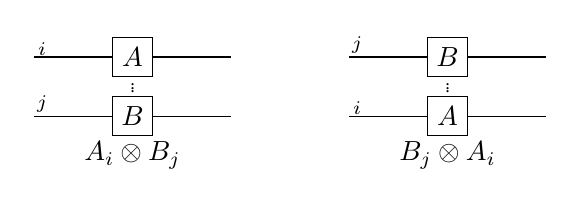
\begin{tikzpicture}
            \draw (0, 0) rectangle (0.5, 0.5) node[midway] {$A$};
            \draw (0, -0.75) rectangle (0.5, -0.25) node[midway] {$B$};
            \draw[-] (-1, 0.25) -- (0, 0.25);
            \draw[-] (-1, -0.5) -- (0, -0.5);
            \node at (-0.9, 0.35) {\scriptsize{$i$}};
            \node at (-0.9, -0.35) {\scriptsize{$j$}};
            \node at (0.25, -1) {$A_i \otimes B_j$};
            \draw[-] (0.5, 0.25) -- (1.5, 0.25);
            \draw[-] (0.5, -0.5) -- (1.5, -0.5);
            \node at (0.25, -0.1) {\scriptsize{$\cdot$}};
            \node at (0.25, -0.15) {\scriptsize{$\cdot$}};
            \node at (0.25, -0.2) {\scriptsize{$\cdot$}};

            \draw (4, 0) rectangle (4.5, 0.5) node[midway] {$B$};
            \draw (4, -0.75) rectangle (4.5, -0.25) node[midway] {$A$};
            \draw[-] (3, 0.25) -- (4, 0.25);
            \draw[-] (3, -0.5) -- (4, -0.5);
            \node at (3.1, 0.4) {\scriptsize{$j$}};
            \node at (3.1, -0.4) {\scriptsize{$i$}};
            \node at (4.25, -1) {$B_j \otimes A_i$};
            \draw[-] (4.5, 0.25) -- (5.5, 0.25);
            \draw[-] (4.5, -0.5) -- (5.5, -0.5);
            \node at (4.25, -0.1) {\scriptsize{$\cdot$}};
            \node at (4.25, -0.15) {\scriptsize{$\cdot$}};
            \node at (4.25, -0.2) {\scriptsize{$\cdot$}};
        \end{tikzpicture}
    \end{center}
\end{thmBox}
\begin{egBox}{Example 3.6}{3 Parallel Hadamard Gates on 3-Qubit Systems}
    \raggedright
    Let the Hadamard gate be $H = \frac{1}{\sqrt{2}}\begin{bmatrix} 1 & 1 \\ 1 & -1 \end{bmatrix}$.\\
    $\implies$ The tensor product of the Hadamard gate on the 1st, 2nd, and 3rd qubits of a 3-qubit system is:
    \begin{align*}
        H_1 \otimes H_2 \otimes H_3 = H^{\otimes 3} &= \frac{1}{\sqrt{2}}\begin{bmatrix} 1 & 1 \\ 1 & -1 \end{bmatrix} \otimes \frac{1}{\sqrt{2}}\begin{bmatrix} 1 & 1 \\ 1 & -1 \end{bmatrix} \otimes \frac{1}{\sqrt{2}}\begin{bmatrix} 1 & 1 \\ 1 & -1 \end{bmatrix}= \frac{1}{\sqrt{8}}\begin{bmatrix} 1 & 1 & 1 & 1 & 1 & 1 & 1 & 1 \\ 1 & -1 & 1 & -1 & 1 & -1 & 1 & -1 \\ 1 & 1 & -1 & -1 & 1 & 1 & -1 & -1 \\ 1 & -1 & -1 & 1 & 1 & -1 & -1 & 1 \\ 1 & 1 & 1 & 1 & -1 & -1 & -1 & -1 \\ 1 & -1 & 1 & -1 & -1 & 1 & -1 & 1 \\ 1 & 1 & -1 & -1 & -1 & -1 & 1 & 1 \\ 1 & -1 & -1 & 1 & -1 & 1 & 1 & -1 \end{bmatrix}
    \end{align*}
\end{egBox}


For a circuit with $n$ qubits, when we apply a CNOT gate on the $i$-th qubit with the $j$-th qubit as the control qubit:
\begin{align*}
    \text{CNOT}_{i, j} &= \ket{\ldots, x_i, \ldots, x_j \oplus x_i, \ldots} \quad \text{for } i < j\\
    \text{CNOT}_{i, j} &= \ket{\ldots, x_j \oplus x_i, \ldots, x_i, \ldots} \quad \text{for } i > j
\end{align*}
\begin{egBox}{Example 3.7}{CNOT Gate on 3-Qubit Systems}
    \raggedright
    For CNOT gate with the 3rd qubit as the control qubit and the 1st qubit as the target qubit.\\
    $\implies$ The matrix representation is:
    \begin{align*}
        \text{CNOT}_{3, 1} = \begin{bmatrix} 1 & 0 & 0 & 0 & 0 & 0 & 0 & 0 \\ 0 & 0 & 0 & 0 & 0 & 1 & 0 & 0 \\ 0 & 0 & 1 & 0 & 0 & 0 & 0 & 0 \\ 0 & 0 & 0 & 0 & 0 & 0 & 0 & 1 \\ 0 & 0 & 0 & 0 & 1 & 0 & 0 & 0 \\ 0 & 1 & 0 & 0 & 0 & 0 & 0 & 0 \\ 0 & 0 & 0 & 1 & 0 & 0 & 1 & 0 \\ 0 & 0 & 0 & 0 & 0 & 0 & 0 & 0 \end{bmatrix}
    \end{align*}
\end{egBox}


\chapter{Grover's Search Algorithm}
\textcolor{magenta}{\section{\textbf{Search Problem}}}
Suppose we have an n-bit string $x$ as input and output a function $f:\{0, 1\}^n \rightarrow \{0, 1\}$ such that $f(x) = 1$ if $x$ is the solution $s$ and $f(x) = 0$ otherwise. Our goal is to find the solution $s$ such that $f(s) = 1$.\\
\vspace{2mm}
We access the function $f$ with an oracle $U_f$ which is a unitary operator that acts as:
\begin{align*}
    U_f\ket{x} = \begin{cases}
        \ket{x} & \text{if } f(x) = 0\\
        -\ket{x} & \text{if } f(x) = 1
    \end{cases} = (-1)^{f(x)}\ket{x}
\end{align*}
Grover's Search Algorithm is a quantum algorithm that can search an unsorted database of $N$ items in $O(\sqrt{N})$ time.

\textcolor{magenta}{\section{\textbf{Grover's Search Algorithm}}}
\subsection{Steps of Grover's Search Algorithm}
The steps of Grover's Search Algorithm are as follows:
\begin{enumerate}
    \item Initialize the system to the uniform superposition of all possible states:
    \[
        \ket{\psi_0} = \frac{1}{\sqrt{N}} \sum_{x=0}^{N-1} \ket{x}
    \]
    \item Apply the oracle $U_f$ to the state $\ket{\psi_0}$:
    \[
        \ket{\psi_1} = U_f\ket{\psi_0} = \frac{1}{\sqrt{N}} \sum_{x=0}^{N-1} (-1)^{f(x)}\ket{x}
    \]
    \item Apply the Grover diffusion operator $G$ to the state $\ket{\psi_1}$:
    \[
        G = 2\ket{\psi_0}\bra{\psi_0} - I
    \]
    \item Repeat steps 2 and 3 for $k$ iterations, where $k = \frac{\pi}{4}\sqrt{\frac{N}{M}}$ and $M$ is the number of solutions to the search problem.
    \item Measure the final state $\ket{\psi_k}$ to obtain the solution $s$.
    \[
        \ket{\psi_k} = G^k U_f^k \ket{\psi_0}
    \]
\end{enumerate}
\begin{center}
    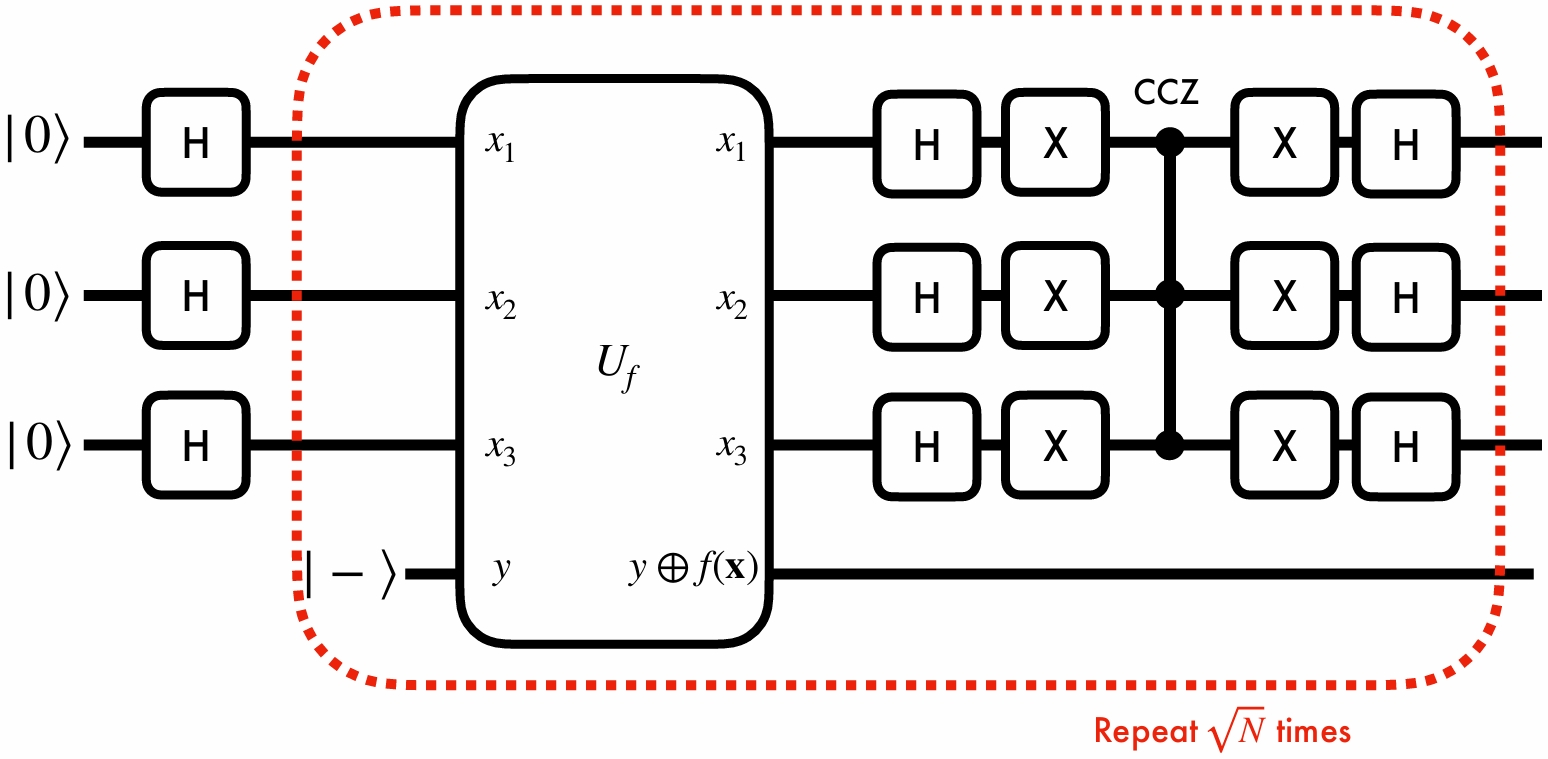
\includegraphics[scale = 0.18]{ch4/ch4_figure1.jpeg}
\end{center}
\newpage
\subsection{Geometric Interpretation of Grover's Search Algorithm}
First, we consider the quantum state space spanned by two vectors $\ket{\alpha} = \frac{1}{\sqrt{N}} \sum_{x=0}^{N-1} \ket{x}$ and $\ket{\beta} = \ket{x_0}$, where $\ket{x_0}$ is the target state.\\
$\implies$ The initial state $\ket{\psi_0}$ is represented as:
\begin{align*}
    \ket{\psi_0} = \sqrt{\frac{N - 1}{N}} \ket{\alpha} + \sqrt{\frac{1}{N}} \ket{\beta} = \cos(\theta)\ket{\alpha} + \sin(\theta)\ket{\beta}
\end{align*}
The angle between $\ket{\psi_0}$ and $\ket{\alpha}$ proves that:
\[
    \sin (\theta) = \sqrt{\frac{1}{N}} \quad \text{and} \quad \cos(\theta) = \sqrt{\frac{N - 1}{N}} \quad \text{where } \theta = \arcsin\left(\frac{1}{\sqrt{N}}\right)
\]
$\implies$ This leads to $\sin(2\theta) = 2\sin(\theta)\cos(\theta) = \frac{2\sqrt{N - 1}}{N}$.\\
\vspace{2mm}
Here is the operations of Grover's Search Algorithm with the geometric interpretation:
\begin{itemize}
    \item After the first operation (from function $f$ to operator $U_f$), the state $\ket{\psi_0}$ is transformed to $\ket{\psi'}$ by applying a phase flip on the target state $\ket{\beta}$:
    \[
        \ket{\psi'} = U_f\ket{\psi_0} = \sqrt{\frac{N - 1}{N}} \ket{\alpha} - \sqrt{\frac{1}{N}} \ket{\beta} = \cos(\theta)\ket{\alpha} - \sin(\theta)\ket{\beta}
    \]
    \item After the second operation (inversion about the mean), the state $\ket{\psi'}$ is transformed to $\ket{\psi_1}$ by reflecting through the average amplitude, flipping around the initial state $\ket{\psi_0}$:
    \[
        \ket{\psi_1} = G\ket{\psi'} = \sqrt{\frac{N - 1}{N}} \ket{\alpha} + \sqrt{\frac{1}{N}} \ket{\beta} = \cos(\theta)\ket{\alpha} + \sin(\theta)\ket{\beta}
    \]
    \item Each iteration of Grover's Search Algorithm consists of applying the oracle $U_f$ and the Grover diffusion operator $G$ to the state $\ket{\psi_k}$, which rotates the state vector by an angle of $2\theta$ in the direction of $\ket{\beta}$:
    \[
        \ket{\psi_{k+1}} = G U_f \ket{\psi_k} = \cos((k + 1)\theta)\ket{\alpha} + \sin((k + 1)\theta)\ket{\beta}
    \]
    \begin{center}
        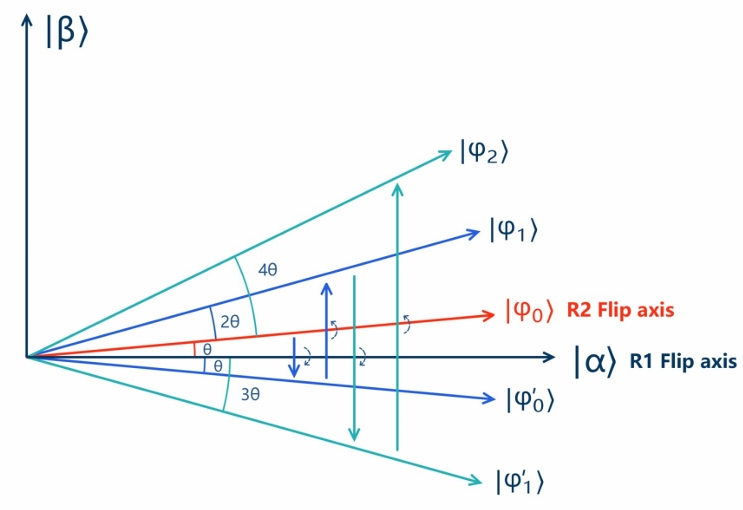
\includegraphics[scale = 0.3]{ch4/ch4_figure2.jpeg}
    \end{center}
\end{itemize}
For large $N$, the angle $\theta$ is small, and the number of iterations $k$ is approximately $\frac{\pi}{4}\sqrt{N}$ to rotate the state vector $\ket{\beta}$ with a probability of $\frac{1}{2}$ to the target state $\ket{x_0}$.\\
\newpage
\subsection{Circuit Representation of Grover's Search Algorithm}
The circuit of Grover's Search Algorithm for $N$ iterations contains the following components:
\begin{itemize}
    \item Hadamard gates on all qubits to create the uniform superposition of all possible states.
    \item Oracle $U_f$ to mark the target state.
    \item Gate $I - 2A$ to invert the amplitude of the target state.
    \item Repeat the oracle and inversion steps for $\sqrt{2^N}$ iterations.
\end{itemize}
The circuit representation of Grover's Search Algorithm is as follows:
\begin{center}
    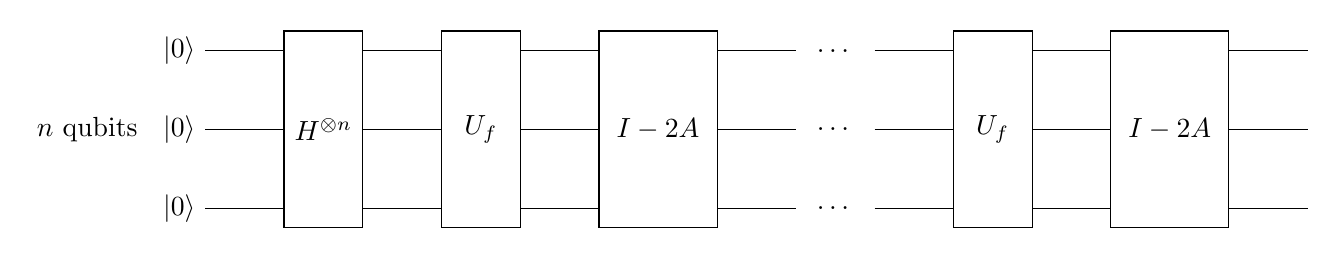
\begin{tikzpicture}
        \node at (-1.5, -1) {$n$ qubits};
        \node at (0, 0) [left] {$\ket{0}$};
        \node at (0, -1) [left] {$\ket{0}$};
        \node at (0, -2) [left] {$\ket{0}$};
        \draw [-] (0, 0) -- (1, 0);
        \draw [-] (0, -1) -- (1, -1);
        \draw [-] (0, -2) -- (1, -2);
        \draw (1, -2.25) rectangle (2, 0.25) node[midway] {$H^{\otimes n}$};
        \draw [-] (2, 0) -- (3, 0);
        \draw [-] (2, -1) -- (3, -1);
        \draw [-] (2, -2) -- (3, -2);
        \draw (3, -2.25) rectangle (4, 0.25) node[midway] {$U_f$};
        \draw [-] (4, 0) -- (5, 0);
        \draw [-] (4, -1) -- (5, -1);
        \draw [-] (4, -2) -- (5, -2);
        \draw (5, -2.25) rectangle (6.5, 0.25) node[midway] {$I - 2A$};
        \draw [-] (6.5, 0) -- (7.5, 0);
        \draw [-] (6.5, -1) -- (7.5, -1);
        \draw [-] (6.5, -2) -- (7.5, -2);
        \node at (8, 0) {$\dots$};
        \node at (8, -1) {$\dots$};
        \node at (8, -2) {$\dots$};
        \draw [-] (8.5, 0) -- (9.5, 0);
        \draw [-] (8.5, -1) -- (9.5, -1);
        \draw [-] (8.5, -2) -- (9.5, -2);
        \draw (9.5, -2.25) rectangle (10.5, 0.25) node[midway] {$U_f$};
        \draw [-] (10.5, 0) -- (11.5, 0);
        \draw [-] (10.5, -1) -- (11.5, -1);
        \draw [-] (10.5, -2) -- (11.5, -2);
        \draw (11.5, -2.25) rectangle (13, 0.25) node[midway] {$I- 2A$};
        \draw [-] (13, 0) -- (14, 0);
        \draw [-] (13, -1) -- (14, -1);
        \draw [-] (13, -2) -- (14, -2);
    \end{tikzpicture}
\end{center}
\vspace{5mm}
We mainly consider the cases for $N = 2$ and $N = 3$ qubits. \\
For $N = 2$ qubits, the circuit representation of Grover's Search Algorithm is as follows:
\begin{center}
    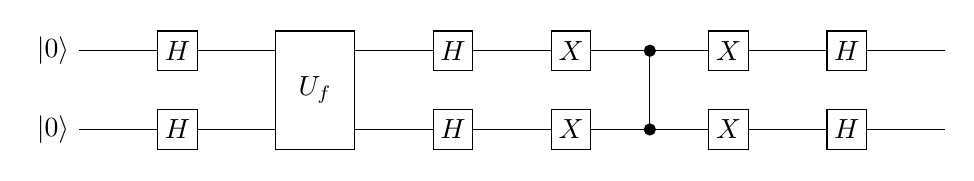
\begin{tikzpicture}
        \node at (-0.5, 0) [left] {$\ket{0}$};
        \node at (-0.5, -1) [left] {$\ket{0}$};
        \draw [-] (-0.5, 0) -- (0.5, 0);
        \draw [-] (-0.5, -1) -- (0.5, -1);
        \draw (0.5, -0.25) rectangle (1, 0.25) node[midway] {$H$};
        \draw (0.5, -1.25) rectangle (1, -0.75) node[midway] {$H$};
        \draw [-] (1, 0) -- (2, 0);
        \draw [-] (1, -1) -- (2, -1);
        \draw (2, -1.25) rectangle (3, 0.25) node[midway] {$U_f$};
        \draw [-] (3, 0) -- (4, 0);
        \draw [-] (3, -1) -- (4, -1);
        \draw (4, -0.25) rectangle (4.5, 0.25) node[midway] {$H$};
        \draw (4, -1.25) rectangle (4.5, -0.75) node[midway] {$H$};
        \draw [-] (4.5, 0) -- (5.5, 0);
        \draw [-] (4.5, -1) -- (5.5, -1);
        \draw (5.5, -0.25) rectangle (6, 0.25) node[midway] {$X$};
        \draw (5.5, -1.25) rectangle (6, -0.75) node[midway] {$X$};
        \draw [-] (6, 0) -- (7.5, 0);
        \draw [-] (6, -1) -- (7.5, -1);
        \draw [-] (6.75, 0) -- (6.75, -1);
        \filldraw (6.75, 0) circle (2pt);
        \filldraw (6.75, -1) circle (2pt);
        \draw (7.5, -0.25) rectangle (8, 0.25) node[midway] {$X$};
        \draw (7.5, -1.25) rectangle (8, -0.75) node[midway] {$X$};
        \draw [-] (8, 0) -- (9, 0);
        \draw [-] (8, -1) -- (9, -1);
        \draw (9, -0.25) rectangle (9.5, 0.25) node[midway] {$H$};
        \draw (9, -1.25) rectangle (9.5, -0.75) node[midway] {$H$};
        \draw [-] (9.5, 0) -- (10.5, 0);
        \draw [-] (9.5, -1) -- (10.5, -1);
    \end{tikzpicture}
\end{center}
For $N = 3$ qubits, the circuit representation of Grover's Search Algorithm is as follows:
\begin{center}
    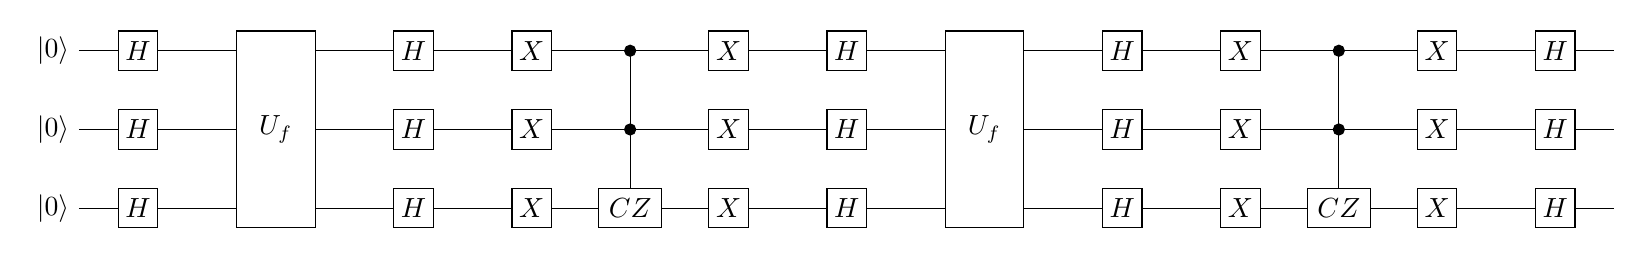
\begin{tikzpicture}
        \node at (0.5, 0) [left] {$\ket{0}$};
        \node at (0.5, -1) [left] {$\ket{0}$};
        \node at (0.5, -2) [left] {$\ket{0}$};
        \draw [-] (0.5, 0) -- (1, 0);
        \draw [-] (0.5, -1) -- (1, -1);
        \draw [-] (0.5, -2) -- (1, -2);
        \draw (1, -0.25) rectangle (1.5, 0.25) node[midway] {$H$};
        \draw (1, -1.25) rectangle (1.5, -0.75) node[midway] {$H$};
        \draw (1, -2.25) rectangle (1.5, -1.75) node[midway] {$H$};
        \draw [-] (1.5, 0) -- (2.5, 0);
        \draw [-] (1.5, -1) -- (2.5, -1);
        \draw [-] (1.5, -2) -- (2.5, -2);
        \draw (2.5, -2.25) rectangle (3.5, 0.25) node[midway] {$U_f$};
        \draw [-] (3.5, 0) -- (4.5, 0);
        \draw [-] (3.5, -1) -- (4.5, -1);
        \draw [-] (3.5, -2) -- (4.5, -2);
        \draw (4.5, -0.25) rectangle (5, 0.25) node[midway] {$H$};
        \draw (4.5, -1.25) rectangle (5, -0.75) node[midway] {$H$};
        \draw (4.5, -2.25) rectangle (5, -1.75) node[midway] {$H$};
        \draw [-] (5, 0) -- (6, 0);
        \draw [-] (5, -1) -- (6, -1);
        \draw [-] (5, -2) -- (6, -2);
        \draw (6, -0.25) rectangle (6.5, 0.25) node[midway] {$X$};
        \draw (6, -1.25) rectangle (6.5, -0.75) node[midway] {$X$};
        \draw (6, -2.25) rectangle (6.5, -1.75) node[midway] {$X$};
        \draw [-] (6.5, 0) -- (8.5, 0);
        \draw [-] (6.5, -1) -- (8.5, -1);
        \draw [-] (6.5, -2) -- (7.1, -2);
        \draw (7.1, -2.25) rectangle (7.9, -1.75) node[midway] {$CZ$};
        \draw (7.9, -2) -- (8.5, -2);
        \draw (7.5, 0) -- (7.5, -1.75);
        \filldraw (7.5, 0) circle (2pt);
        \filldraw (7.5, -1) circle (2pt);
        \draw (8.5, -0.25) rectangle (9, 0.25) node[midway] {$X$};
        \draw (8.5, -1.25) rectangle (9, -0.75) node[midway] {$X$};
        \draw (8.5, -2.25) rectangle (9, -1.75) node[midway] {$X$};
        \draw [-] (9, 0) -- (10, 0);
        \draw [-] (9, -1) -- (10, -1);
        \draw [-] (9, -2) -- (10, -2);
        \draw (10, -0.25) rectangle (10.5, 0.25) node[midway] {$H$};
        \draw (10, -1.25) rectangle (10.5, -0.75) node[midway] {$H$};
        \draw (10, -2.25) rectangle (10.5, -1.75) node[midway] {$H$};
        \draw [-] (10.5, 0) -- (11.5, 0);
        \draw [-] (10.5, -1) -- (11.5, -1);
        \draw [-] (10.5, -2) -- (11.5, -2);
        \draw (11.5, -2.25) rectangle (12.5, 0.25) node[midway] {$U_f$};
        \draw [-] (12.5, 0) -- (13.5, 0);
        \draw [-] (12.5, -1) -- (13.5, -1);
        \draw [-] (12.5, -2) -- (13.5, -2);
        \draw (13.5, -0.25) rectangle (14, 0.25) node[midway] {$H$};
        \draw (13.5, -1.25) rectangle (14, -0.75) node[midway] {$H$};
        \draw (13.5, -2.25) rectangle (14, -1.75) node[midway] {$H$};
        \draw [-] (14, 0) -- (15, 0);
        \draw [-] (14, -1) -- (15, -1);
        \draw [-] (14, -2) -- (15, -2);
        \draw (15, -0.25) rectangle (15.5, 0.25) node[midway] {$X$};
        \draw (15, -1.25) rectangle (15.5, -0.75) node[midway] {$X$};
        \draw (15, -2.25) rectangle (15.5, -1.75) node[midway] {$X$};
        \draw [-] (15.5, 0) -- (17.5, 0);
        \draw [-] (15.5, -1) -- (17.5, -1);
        \draw [-] (15.5, -2) -- (16.1, -2);
        \draw (16.1, -2.25) rectangle (16.9, -1.75) node[midway] {$CZ$};
        \draw (16.9, -2) -- (17.5, -2);
        \draw (16.5, 0) -- (16.5, -1.75);
        \filldraw (16.5, 0) circle (2pt);
        \filldraw (16.5, -1) circle (2pt);
        \draw (17.5, -0.25) rectangle (18, 0.25) node[midway] {$X$};
        \draw (17.5, -1.25) rectangle (18, -0.75) node[midway] {$X$};
        \draw (17.5, -2.25) rectangle (18, -1.75) node[midway] {$X$};
        \draw [-] (18, 0) -- (19, 0);
        \draw [-] (18, -1) -- (19, -1);
        \draw [-] (18, -2) -- (19, -2);
        \draw (19, -0.25) rectangle (19.5, 0.25) node[midway] {$H$};
        \draw (19, -1.25) rectangle (19.5, -0.75) node[midway] {$H$};
        \draw (19, -2.25) rectangle (19.5, -1.75) node[midway] {$H$};
        \draw [-] (19.5, 0) -- (20, 0);
        \draw [-] (19.5, -1) -- (20, -1);
        \draw [-] (19.5, -2) -- (20, -2);
    \end{tikzpicture}
\end{center}



\chapter{Complex Numbers and Bloch Sphere}
\textcolor{magenta}{\section{\textbf{Complex Numbers}}}
\subsection{Definition and Operations of Complex Numbers}
\begin{defBox}{Definition 5.1}{Complex Numbers}
    A complex number is a number of the form $\boxed{\textcolor{teal}{z = a + bi}}$ where $a, b \in \mathbb{R}$ and $\boxed{\textcolor{red}{i = \sqrt{-1}}}$.\\
    The real part of $z$ is denoted by \textcolor{purple}{$\Re(z) = a$} and the imaginary part of $z$ is denoted by \textcolor{purple}{$\Im(z) = b$}.
\end{defBox}
The operations on complex numbers are as follows:
\begin{itemize}
    \item Addition: $z_1 + z_2 = (a_1 + a_2) + (b_1 + b_2)i$
    \item Subtraction: $z_1 - z_2 = (a_1 - a_2) + (b_1 - b_2)i$
    \item Multiplication: $z_1 \cdot z_2 = (a_1a_2 - b_1b_2) + (a_1b_2 + a_2b_1)i$
    \item Division: $\frac{z_1}{z_2} = \frac{(a_1a_2 + b_1b_2) + (b_1a_2 - a_1b_2)i}{a^2 + b^2}$
    \item Modulus: $|z| = \sqrt{a^2 + b^2}$
    \item Argument: $\arg(z) = \tan^{-1}\left(\frac{b}{a}\right)$, which is the angle between the positive real axis and the line connecting the origin to the point $(a, b)$ in the complex plane.
    \item Complex Conjugate: $\bar{z} = a - bi$
    \item Exponential Form: $z = re^{i\theta}$ where $r = |z|$ and $\theta = \arg(z)$
    \item Polar Form: $z = r(\cos(\theta) + i\sin(\theta))$ where $r = |z|$ and $\theta = \arg(z)$
\end{itemize}
\vspace{2mm}
The 4 roots of unity are the complex numbers that satisfy the equation $z^4 = 1$. They are \hl{$1, i, -1, -i$} and can be represented in polar form as:
\begin{align*}
    \boxed{z_0 = 1 = e^{i0}} \quad, \quad \boxed{z_1 = i = e^{i\frac{\pi}{2}}} \quad, \quad \boxed{z_2 = -1 = e^{i\pi}} \quad, \quad \boxed{z_3 = -i = e^{i\frac{3\pi}{2}}}
\end{align*}
\subsection{Euler's Formula}
\begin{thmBox}{Theorem 5.1}{Euler's Formula}
    \textcolor{red}{Euler's formula} states that for any real number $\theta$:
    \[
        \boxed{\textcolor{teal}{e^{i\theta} = \cos(\theta) + i\sin(\theta)}}
    \]
    $\implies$ Relate the complex exponential function to the trigonometric functions cosine and sine.
\end{thmBox}
The proof of Euler's formula can be derived from the Taylor series expansions of the exponential function, cosine, and sine:
\begin{align*}
    e^{i\theta} = \sum_{n=0}^{\infty} \frac{(i\theta)^n}{n!} = 1 + i\theta + \frac{(i\theta)^2}{2!} + \frac{(i\theta)^3}{3!} + \cdots = 1 + i\theta - \frac{\theta^2}{2!} - i\frac{\theta^3}{3!} + \cdots &= \left(1 - \frac{\theta^2}{2!} + \frac{\theta^4}{4!} - \cdots\right) + i\left(\theta - \frac{\theta^3}{3!} + \frac{\theta^5}{5!} - \cdots\right)\\
    &= \cos(\theta) + i\sin(\theta)
\end{align*}
\newpage
\subsection{Polar Form of Complex Numbers}
\begin{thmBox}{Theorem 5.2}{Polar Form of Complex Numbers}
    The polar form of a complex number $z = a + bi$ is given by:
    \[
        \boxed{\textcolor{red}{z = re^{i\theta}}} \quad \text{where } \boxed{\textcolor{teal}{r = |z| = \sqrt{a^2 + b^2}}} \text{ and } \boxed{\textcolor{teal}{\theta = \arg(z) = \tan^{-1}\left(\frac{b}{a}\right)}}
    \]
    \begin{center}
        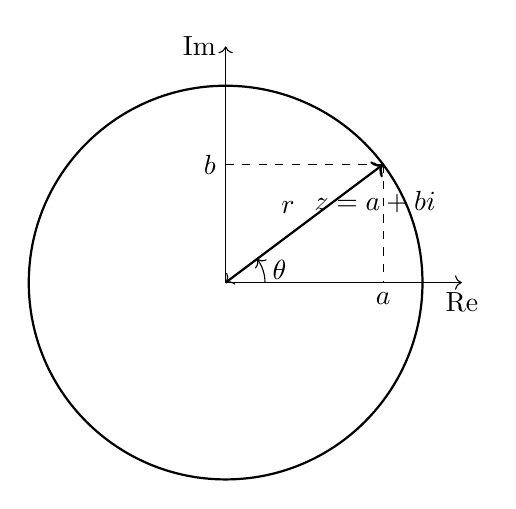
\begin{tikzpicture}
            \draw[->] (0,0) -- (3,0) node[anchor=north] {Re};
            \draw[->] (0,0) -- (0,3) node[anchor=east] {Im};
            \draw[->, thick] (0,0) -- (2,1.5) node[midway, above right] {$z = a + bi$};
            \draw[dashed] (2,1.5) -- (2,0) node[anchor=north] {$a$};
            \draw[dashed] (2,1.5) -- (0,1.5) node[anchor=east] {$b$};
            \draw[thick] (0,0) circle (2.5cm);
            \draw[->] (0.5,0) arc[start angle=0, end angle=37, radius=0.5cm] node[midway, right] {$\theta$};
            \draw[<->] (0,0) -- (2,1.5) node[midway, above left] {$r$};
        \end{tikzpicture}
    \end{center}
\end{thmBox}
The polar form of complex numbers allows us to express them in terms of their modulus and argument, which can simplify calculations involving multiplication and division.\\
\begin{itemize}
    \item Multiplication: $z_1 \cdot z_2 = r_1r_2 e^{i(\theta_1 + \theta_2)}$
    \item Division: $\frac{z_1}{z_2} = \frac{r_1}{r_2} e^{i(\theta_1 - \theta_2)}$
    \item Conjugate: $\bar{z} = re^{-i\theta}$
    \item Modulus: $|z| = r$
    \item Argument: $\arg(z) = \theta$
\end{itemize}
\textcolor{magenta}{\section{\textbf{Bloch Sphere}}}
\subsection{Definition and Representation of Bloch Sphere}
\begin{defBox}{Definition 5.2}{Bloch Sphere}
    The \textcolor{red}{Bloch sphere} is a geometrical representation of a qubit state in a three-dimensional space.\\
    A qubit state can be represented as:
    \[
        \boxed{\textcolor{teal}{\ket{\psi} = \cos\left(\frac{\theta}{2}\right)\ket{0} + e^{i\phi}\sin\left(\frac{\theta}{2}\right)\ket{1}}}
    \]
    where $\theta$ is the polar angle and $\phi$ is the azimuthal angle.
\end{defBox}
The Bloch sphere is a unit sphere in three-dimensional space, which has the following properties:
\begin{wrapfigure}[6]{r}{0.25\textwidth}
        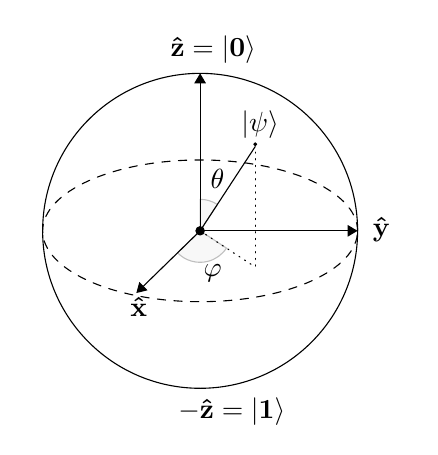
\begin{tikzpicture}[line cap=round, line join=round, >=Triangle]
  \clip(-2.19,-2.49) rectangle (2.66,2.58);
  \draw [shift={(0,0)}, lightgray, fill, fill opacity=0.1] (0,0) -- (56.7:0.4) arc (56.7:90.:0.4) -- cycle;
  \draw [shift={(0,0)}, lightgray, fill, fill opacity=0.1] (0,0) -- (-135.7:0.4) arc (-135.7:-33.2:0.4) -- cycle;
  \draw(0,0) circle (2cm);
  \draw [rotate around={0.:(0.,0.)},dash pattern=on 3pt off 3pt] (0,0) ellipse (2cm and 0.9cm);
  \draw (0,0)-- (0.70,1.07);
  \draw [->] (0,0) -- (0,2);
  \draw [->] (0,0) -- (-0.81,-0.79);
  \draw [->] (0,0) -- (2,0);
  \draw [dotted] (0.7,1)-- (0.7,-0.46);
  \draw [dotted] (0,0)-- (0.7,-0.46);
  \draw (-0.08,-0.3) node[anchor=north west] {$\varphi$};
  \draw (0.01,0.9) node[anchor=north west] {$\theta$};
  \draw (-1.01,-0.72) node[anchor=north west] {$\mathbf {\hat{x}}$};
  \draw (2.07,0.3) node[anchor=north west] {$\mathbf {\hat{y}}$};
  \draw (-0.5,2.6) node[anchor=north west] {$\mathbf {\hat{z}=|0\rangle}$};
  \draw (-0.4,-2) node[anchor=north west] {$-\mathbf {\hat{z}=|1\rangle}$};
  \draw (0.4,1.65) node[anchor=north west] {$|\psi\rangle$};
  \scriptsize
  \draw [fill] (0,0) circle (1.5pt);
  \draw [fill] (0.7,1.1) circle (0.5pt);
\end{tikzpicture}
\end{wrapfigure}
\begin{itemize}
    \item The north pole of the Bloch sphere represents the state $\ket{0}$.
    \item The south pole of the Bloch sphere represents the state $\ket{1}$.
    \item The equator of the Bloch sphere represents the superposition states of the qubit.
    \item The points on the surface of the Bloch sphere represent all possible pure states of a qubit.
    \item The center of the Bloch sphere represents the mixed states of a qubit.
    \item The radius of the Bloch sphere is 1, which represents the normalization condition of the qubit state.
    \item The angles $\theta$ and $\phi$ are related to the probability amplitudes of the qubit state.
\end{itemize}

\newpage
\subsection{Operations on the Bloch Sphere}
The sphereical coordinates of the Bloch sphere can be expressed in terms of the Cartesian coordinates as:
\begin{align*}
    \boxed{x = \sin(\theta)\cos(\phi)} \quad, \quad \boxed{y = \sin(\theta)\sin(\phi)} \quad \text{and} \quad \boxed{z = \cos(\theta)}
\end{align*}
$\implies$ The squared radius of the Bloch sphere is $\boxed{\textcolor{teal}{r^2 = x^2 + y^2 + z^2 = 1}}$.\\
\vspace{2mm}
For $X, Y, Z$ gates, 







\subsection{Rotations on the Bloch Sphere}
\begin{thmBox}{Theorem 5.3}{Rotations on the Bloch Sphere}
    The rotation of a qubit state on the Bloch sphere can be represented by the following unitary operators:
    \begin{itemize}
        \item Rotation around the $z$-axis:
        \[
            R_z(\phi) = e^{-i\frac{\phi}{2}\sigma_z} = \cos\left(\frac{\phi}{2}\right)I - i\sin\left(\frac{\phi}{2}\right)\sigma_z
        \]
        \item Rotation around the $x$-axis:
        \[
            R_x(\theta) = e^{-i\frac{\theta}{2}\sigma_x} = \cos\left(\frac{\theta}{2}\right)I - i\sin\left(\frac{\theta}{2}\right)\sigma_x
        \]
        \item Rotation around the $y$-axis:
        \[
            R_y(\theta) = e^{-i\frac{\theta}{2}\sigma_y} = \cos\left(\frac{\theta}{2}\right)I - i\sin\left(\frac{\theta}{2}\right)\sigma_y
        \]
    \end{itemize}
    where $\sigma_x$, $\sigma_y$, and $\sigma_z$ are the Pauli matrices.
\end{thmBox}




\chapter{Quantum Gates as Unitary Operators}

\textcolor{magenta}{\section{\textbf{Unitary Matrices}}}

\begin{defBox}{Definition 6.1}{Unitary Matrices}
A matrix $U \in \mathbb{C}^{n \times n}$ is \textbf{\textcolor{cyan}{unitary}} if
$\boxed{\textcolor{red}{U U^\dagger = U^\dagger U = I_n}} \quad \text{where } U^\dagger \text{ is the conjugate transpose (adjoint) of } U$.
\end{defBox}
Unitary matrices \hl{preserve inner products and correspond to reversible quantum evolutions}.\\
\vspace{2mm}
There are two examples of unitary matrices: 
\begin{itemize}
    \item \textbf{Pauli Matrices} (all unitary and Hermitian): $
    X = \begin{bmatrix} 0 & 1 \\ 1 & 0 \end{bmatrix}, \quad
    Y = \begin{bmatrix} 0 & -i \\ i & 0 \end{bmatrix}, \quad
    Z = \begin{bmatrix} 1 & 0 \\ 0 & -1 \end{bmatrix}$.
    \item \textbf{Rotation Matrices} (unitary): $R_z(\theta) = \begin{bmatrix} e^{-i\frac{\theta}{2}} & 0 \\ 0 & e^{i\frac{\theta}{2}} \end{bmatrix}$.
\end{itemize}

There are some properties of any unitary matrix $U$:
\begin{itemize}
    \item \textcolor{blue}{Invertibility}: $\boxed{U U^{-1} = U^{1} U = I_n}$ , which means $U^{-1} = U^\dagger$.
    \item \textcolor{blue}{Transpose}: $\boxed{U^T[j,k] = U[k,j]}$ .
    \item \textcolor{blue}{Conjugate}: $\boxed{\overline{U}[j,k] = \overline{U[j,k]}}$.
    \item \textcolor{blue}{Adjoint (Conjugate Transpose)}: $\boxed{U^\dagger[j,k] = \overline{U[k,j]}}$.
\end{itemize}

\textcolor{magenta}{\section{\textbf{Quantum Controlled Gates}}}

\subsection{Controlled Gates' Matrices}
There are some controlled gates that are used in quantum computing. The controlled gates are \textcolor{purple}{unitary operations that act on two qubits, where one qubit is the control qubit and the other is the target qubit}. The controlled gates can be represented by their matrices.\\
The controlled gates are defined as follows:
\begin{itemize}
    \item \textbf{\textcolor{cyan}{Controlled-NOT (CNOT) / Controlled-X (CX)}}: $\boxed{\textcolor{red}{\text{CNOT} \ket{x}\ket{y} = \ket{x}\ket{y \oplus x}}}$, where $\oplus$ is the XOR operation.\\
    $\implies$ The CNOT gate matrix is:
    \[
    \begin{bmatrix}
    1 & 0 & 0 & 0 \\
    0 & 1 & 0 & 0 \\
    0 & 0 & 0 & 1 \\
    0 & 0 & 1 & 0
    \end{bmatrix}
    \]
    \item \textbf{\textcolor{cyan}{Controlled-Z (CZ)}}: $\boxed{\textcolor{red}{\text{CZ} \ket{x}\ket{y} = (-1)^{xy}\ket{x}\ket{y}}}$ .\\
    $\implies$ The CZ gate matrix is:
    \[
    \begin{bmatrix}
    1 & 0 & 0 & 0 \\
    0 & 1 & 0 & 0 \\
    0 & 0 & 1 & 0 \\
    0 & 0 & 0 & -1
    \end{bmatrix}
    \]
    \item \textbf{\textcolor{cyan}{Controlled-U (CU)}}: $\boxed{\textcolor{red}{\bar{0}\ket{0} \otimes I + \bar{1}\ket{1} \otimes U}}$, where $U$ is a unitary matrix.\\
    The CU gate matrix is:
    \[
    \begin{bmatrix}
    1 & 0 & 0 & 0 \\
    0 & 1 & 0 & 0 \\
    0 & 0 & u_{00} & u_{01} \\
    0 & 0 & u_{10} & u_{11}
    \end{bmatrix}
    \]
\end{itemize}

\subsection{Decomposition of Controlled Gates}
Any controlled-$U$ can be constructed from CNOT and single-qubit gates. For any single-qubit unitary $U$, there exist single-qubit gates $A$, $B$, $C$ and a phase $\alpha$ such that
\[
U = e^{i\alpha} A X B X C, \quad \text{with } ABC = I
\]
where $X$ is the Pauli-X gate. The decomposition is:
\begin{align*}
A &= R_z(\beta) R_y(\gamma/2) \\
B &= R_y(-\gamma/2) R_z(-(\delta+\beta)/2) \\
C &= R_z((\delta-\beta)/2)
\end{align*}

\section{Universality of Quantum Gates}

\subsection{Universal Gate Sets}
\begin{thmBox}{Theorem 6.1}{Universality of Quantum Gates}
Any unitary operation on $n$ qubits can be approximated to arbitrary accuracy using only:
\begin{itemize}
    \item Single-qubit gates
    \item CNOT gates
\end{itemize}
\end{thmBox}

\subsection{Examples of Universal Gate Sets}
\begin{itemize}
    \item $\{H, T, \text{CNOT}\}$, where $T = \begin{bmatrix} 1 & 0 \\ 0 & e^{i\pi/4} \end{bmatrix}$
    \item $\{\text{Toffoli}, H\}$
\end{itemize}

\subsection{Toffoli Gate Construction}
The Toffoli (CCNOT) gate can be constructed from controlled-Z and Hadamard gates:
\[
\text{Toffoli} = (I \otimes H)\,\text{CCZ}\,(I \otimes H)
\]
where CCZ is the doubly-controlled-Z gate.






\chapter{Quantum Fourier Transform}
\textcolor{magenta}{\section{\textbf{Definition of Quantum Fourier Transform}}}
\begin{defBox}{Definition 7.1}{Quantum Fourier Transform}
    The \textcolor{red}{Quantum Fourier Transform (QFT)} is a quantum algorithm that linearly transforms a quantum state from the computational basis to the Fourier basis.\\
    The QFT of an $n$-qubit state $\ket{x}$ is defined as:
    \[
        \boxed{\textcolor{teal}{QFT(\ket{x}) = \frac{1}{\sqrt{2^n}} \sum_{k=0}^{2^n - 1} e^{2\pi i \frac{xy}{2^n}} \ket{k}}}
    \]
    where $x$ is the input state and $k$ is the output state.
\end{defBox}
The QFT can be represented by an unitary matrix $U_{QFT}$, which is an $N \times N$ matrix where $N = 2^n$:
\[
    \boxed{\textcolor{teal}{U_{QFT} = \frac{1}{\sqrt{N}} \begin{bmatrix} 
        1 & 1 & 1 & \cdots & 1 \\
        1 & \omega & \omega^2 & \cdots & \omega^{N-1} \\
        1 & \omega^2 & \omega^4 & \cdots & \omega^{2(N-1)} \\
        \vdots & \vdots & \vdots & \ddots & \vdots \\
        1 & \omega^{N-1} & \omega^{2(N-1)} & \cdots & \omega^{(N-1)(N-1)}
    \end{bmatrix}}} \quad \text{where } \omega = e^{2\pi i / N}
\]
The QFT can be implemented using a series of Hadamard gates and controlled phase gates. The QFT algorithm has a time complexity of $O(n^2)$, which is exponentially faster than the classical Fourier transform algorithm with a time complexity of $O(n2^n)$.









\chapter{Quantum Communication and Cryptography}

\section{Classical and Quantum Key Distribution}

\subsection{One-Time Pad Protocol (Classical)}
A one-time pad is a classical encryption method that provides perfect secrecy if the key is truly random, used only once, and kept secret.

\begin{itemize}
    \item Let $T$ be the original message (a binary string of length $n$).
    \item Let $K$ be a random key of length $n$ shared by Alice and Bob.
    \item Alice computes the encrypted message $E = T \oplus K$ and sends $E$ over a public channel.
    \item Bob decrypts by computing $T = E \oplus K$.
\end{itemize}

\subsection{Limitations of Classical Key Distribution}
In classical communication, an eavesdropper (Eve) can copy the transmitted data without detection and store it for later analysis. This makes secure key distribution challenging.

\subsection{Quantum Key Distribution (QKD) Motivation}
Quantum mechanics introduces two key properties:
\begin{itemize}
    \item \textbf{No-Cloning Theorem}: It is impossible to make a perfect copy of an unknown quantum state.
    \item \textbf{Measurement Disturbs State}: Measuring a quantum state generally changes it, so eavesdropping can be detected.
\end{itemize}

\section{Linear Algebra Concepts for Quantum Information}

\subsection{Vectors and Linear Combinations}
A vector $V$ is a linear combination of vectors $V_0, V_1, \ldots, V_{n-1}$ if
\[
V = c_0 V_0 + c_1 V_1 + \cdots + c_{n-1} V_{n-1}
\]
for some complex numbers $c_0, \ldots, c_{n-1}$.

\subsection{Linear Independence and Basis}
A set of vectors $[V_0, V_1, \ldots, V_{n-1}]$ is linearly independent if the only solution to
\[
0 = c_0 V_0 + c_1 V_1 + \cdots + c_{n-1} V_{n-1}
\]
is $c_0 = c_1 = \cdots = c_{n-1} = 0$.

A \textbf{basis} is a set of linearly independent vectors such that any vector in the space can be written as a linear combination of them.

\subsection{Standard Basis}
For $\mathbb{R}^n$ or $\mathbb{C}^n$, the standard basis is
\[
E_0 = 
\begin{bmatrix}
1 \\ 0 \\ \vdots \\ 0
\end{bmatrix},\quad
E_1 = 
\begin{bmatrix}
0 \\ 1 \\ \vdots \\ 0
\end{bmatrix},\quad
\ldots,\quad
E_{n-1} = 
\begin{bmatrix}
0 \\ 0 \\ \vdots \\ 1
\end{bmatrix}
\]
Any vector $[c_0, c_1, \ldots, c_{n-1}]^T$ can be written as $\sum_{j=0}^{n-1} c_j E_j$.

\subsection{Inner Product and Orthonormal Basis}
The inner product of $V_1 = [r_0, \ldots, r_m]^T$ and $V_2 = [r_0', \ldots, r_m']^T$ is
\[
\langle V_1, V_2 \rangle = \sum_{j=0}^m \bar{r}_j r_j'
\]
Vectors are orthogonal if their inner product is zero. An orthonormal basis is a set of vectors that are both orthogonal and of unit length.

\section{Quantum Measurement in Different Bases}
Any quantum state $|\psi\rangle$ can be written in an orthonormal basis $\{|e_i\rangle\}$ as
\[
|\psi\rangle = \sum_{i} c_i |e_i\rangle
\]
Measuring $|\psi\rangle$ in this basis yields outcome $|e_i\rangle$ with probability
\[
p_i = \frac{|c_i|^2}{\sum_j |c_j|^2}
\]

\section{The BB84 Quantum Key Distribution Protocol}

\subsection{Encoding with Two Bases}
The BB84 protocol uses two bases for encoding qubits:
\begin{itemize}
    \item \textbf{Z basis} ($+$): $\{|0\rangle, |1\rangle\} = \{[1,0]^T, [0,1]^T\}$
    \item \textbf{X basis} ($\times$): $\left\{\frac{1}{\sqrt{2}}([1,1]^T), \frac{1}{\sqrt{2}}([-1,1]^T)\right\}$
\end{itemize}

\subsection{Protocol Steps}
\begin{enumerate}
    \item Alice randomly chooses a bit value and a basis for each qubit, prepares the qubit accordingly, and sends it to Bob.
    \item Bob randomly chooses a basis for each qubit and measures.
    \item Alice and Bob publicly compare which bases they used and keep only the bits where their bases matched.
    \item To check for eavesdropping, Bob reveals a random subset of his bits; Alice checks if they match her original bits. If too many errors are found, they abort.
\end{enumerate}

\section{The Bell Basis and Quantum Entanglement}
The Bell basis consists of four maximally entangled two-qubit states:
\begin{align*}
|\Psi^+\rangle &= \frac{|01\rangle + |10\rangle}{\sqrt{2}} \\
|\Psi^-\rangle &= \frac{|01\rangle - |10\rangle}{\sqrt{2}} \\
|\Phi^+\rangle &= \frac{|00\rangle + |11\rangle}{\sqrt{2}} \\
|\Phi^-\rangle &= \frac{|00\rangle - |11\rangle}{\sqrt{2}}
\end{align*}

\section{Quantum Teleportation Protocol}
Quantum teleportation allows the transfer of an unknown quantum state using entanglement and classical communication.

\begin{enumerate}
    \item Alice and Bob share an entangled pair in the $|\Phi^+\rangle$ Bell state.
    \item Alice combines her unknown state $|\psi\rangle$ with her half of the entangled pair and performs a joint measurement (Bell measurement).
    \item Alice sends the result (two classical bits) to Bob.
    \item Bob applies a corresponding unitary operation to his qubit to reconstruct $|\psi\rangle$.
\end{enumerate}

\subsection*{Bob's Correction Operations}
\begin{center}
\begin{tabular}{|c|c|}
\hline
Alice's bits & Bob applies \\
\hline
00 & $I = \begin{bmatrix} 1 & 0 \\ 0 & 1 \end{bmatrix}$ \\
01 & $X = \begin{bmatrix} 0 & 1 \\ 1 & 0 \end{bmatrix}$ \\
10 & $Z = \begin{bmatrix} 1 & 0 \\ 0 & -1 \end{bmatrix}$ \\
11 & $XZ = \begin{bmatrix} 0 & 1 \\ -1 & 0 \end{bmatrix}$ \\
\hline
\end{tabular}
\end{center}



\chapter{Building Quantum Computers}
\section{Physical Realization of Quantum Computers: The Circuit Model}

\subsection*{DiVincenzo Criteria}
To build a quantum computer, a physical system must satisfy the following criteria (DiVincenzo, 2000):
\begin{itemize}
    \item \textbf{Scalable qubits}: A physical system with well-characterized, scalable qubits.
    \item \textbf{Initialization}: Ability to initialize qubits to a known fiducial state.
    \item \textbf{Long coherence times}: Decoherence times much longer than gate-operation times.
    \item \textbf{Universal gates}: Ability to implement a universal set of quantum gates.
    \item \textbf{Measurement}: Qubit-specific measurement capability.
\end{itemize}

\section{Quantum Dynamics and Unitary Evolution}

\subsection*{Postulate: Unitary Evolution}
The evolution of a closed quantum system (excluding measurement) is described by a unitary operator $U$. If $|\psi(t)\rangle$ is the state at time $t$, then
\[
|\psi(t+1)\rangle = U|\psi(t)\rangle.
\]

\subsection*{Schrödinger's Equation}
The time evolution of a quantum state is governed by Schrödinger's equation. For a small time increment $\Delta t$:
\begin{align*}
|\psi(t+\Delta t)\rangle - |\psi(t)\rangle &= -iH\Delta t\,|\psi(t)\rangle \\
|\psi(t+\Delta t)\rangle &= (I - iH\Delta t)\,|\psi(t)\rangle \\
&\approx e^{-iH\Delta t}|\psi(t)\rangle
\end{align*}
Thus, the unitary evolution operator is
\[
U = e^{-iH\Delta t}
\]
where $H$ is the Hamiltonian (energy operator) of the system.

\section{Hamiltonians and Quantum Gates}

\subsection*{Hamiltonian: Definition and Examples}
The Hamiltonian $H$ describes the total energy of the system. Examples:
\begin{itemize}
    \item \textbf{Classical:}
        \begin{itemize}
            \item Kinetic: $H = \frac{p^2}{2m}$
            \item Gravitational: $H = mgh$
            \item Elastic: $H = \frac{1}{2}kx^2$
        \end{itemize}
    \item \textbf{Quantum (spin in magnetic field $B_0$):}
    \[
    H = -\frac{1}{2}\hbar\gamma B_0 Z = -\frac{1}{2}\hbar\omega_0 Z =
    \begin{bmatrix}
    -\frac{1}{2}\hbar\omega_0 & 0 \\
    0 & \frac{1}{2}\hbar\omega_0
    \end{bmatrix}
    \]
\end{itemize}

\section{Hermitian and Unitary Matrices}

\subsection*{Hermitian Matrices}
A matrix $A \in \mathbb{C}^{n \times n}$ is:
\begin{itemize}
    \item \textbf{Symmetric} if $A^T = A$ ($A[j,k] = A[k,j]$).
    \item \textbf{Hermitian} if $A^\dagger = A$ ($A[j,k] = \overline{A[k,j]}$).
\end{itemize}
\textbf{Examples:}
\[
\begin{bmatrix}
5 & 4+5i & 6-16i \\
4-5i & 13 & 7 \\
6+16i & 7 & -2.1
\end{bmatrix}
\]
is Hermitian.

The Pauli matrices
\[
X = \begin{bmatrix} 0 & 1 \\ 1 & 0 \end{bmatrix},\quad
Y = \begin{bmatrix} 0 & -i \\ i & 0 \end{bmatrix},\quad
Z = \begin{bmatrix} 1 & 0 \\ 0 & -1 \end{bmatrix}
\]
are Hermitian.

\subsection*{Unitary Matrices}
A matrix $U \in \mathbb{C}^{n \times n}$ is \textbf{unitary} if
\[
U U^\dagger = U^\dagger U = I_n
\]
\textbf{Property:} If $H$ is Hermitian, then $e^{iH}$ is unitary:
\[
(e^{iH})^\dagger e^{iH} = e^{-iH} e^{iH} = I_n
\]

\textbf{Physical meaning:} To realize a quantum gate $e^{-iH\Delta t}$, engineer the system Hamiltonian $H$ for time $\Delta t$.

\section{NMR Quantum Computing Example}

\subsection*{NMR System and DiVincenzo Criteria}
NMR (Nuclear Magnetic Resonance) systems satisfy the DiVincenzo criteria:
\begin{itemize}
    \item \checkmark Qubits: nuclear spins in $B_0$ field ($\uparrow$ and $\downarrow$ as $0$ and $1$)
    \item \checkmark Quantum gates: RF pulses and delays
    \item (\checkmark) Initialization: Boltzmann distribution at room temperature
    \item \checkmark Measurement: RF coil detection
    \item \checkmark Coherence times: several seconds
\end{itemize}

% \begin{figure}[h]
%     \centering
%     \includegraphics[width=0.6\textwidth]{nmr_system.png}
%     \caption{NMR system components (Gershenfeld \& Chuang 1997, Cory, Havel \& Fahmi 1997)}
% \end{figure}

\subsection*{Single Spin System}
Hamiltonian for a single spin in $B_0$:
\[
H = -\frac{1}{2}\hbar\gamma B_0 Z = -\frac{1}{2}\hbar\omega_0 Z =
\begin{bmatrix}
-\frac{1}{2}\hbar\omega_0 & 0 \\
0 & \frac{1}{2}\hbar\omega_0
\end{bmatrix}
\]

\subsection*{Control Hamiltonian (RF Pulses)}
In the rotating frame, the control Hamiltonian is:
\[
H_c = -\frac{1}{2}\hbar\omega_1(\cos\phi\, X + \sin\phi\, Y)
\]
where $\omega_1 = \gamma B_1$ (RF amplitude), and $\phi$ is the phase. The evolution for pulse width $t_{pw}$:
\[
e^{-iH_c t_{pw}} = e^{-i\frac{1}{2}\hbar\omega_1(\cos\phi\, X + \sin\phi\, Y)t_{pw}}
\]

\section{Single-Qubit Gates as Rotations}
\begin{align*}
R_x(\theta) &= e^{-i\frac{\theta}{2}X} = \cos\frac{\theta}{2}I - i\sin\frac{\theta}{2}X =
\begin{bmatrix}
\cos\frac{\theta}{2} & -i\sin\frac{\theta}{2} \\
-i\sin\frac{\theta}{2} & \cos\frac{\theta}{2}
\end{bmatrix} \\
R_y(\theta) &= e^{-i\frac{\theta}{2}Y} = \cos\frac{\theta}{2}I - i\sin\frac{\theta}{2}Y =
\begin{bmatrix}
\cos\frac{\theta}{2} & -\sin\frac{\theta}{2} \\
\sin\frac{\theta}{2} & \cos\frac{\theta}{2}
\end{bmatrix} \\
R_z(\theta) &= e^{-i\frac{\theta}{2}Z} = \cos\frac{\theta}{2}I - i\sin\frac{\theta}{2}Z =
\begin{bmatrix}
e^{-i\theta/2} & 0 \\
0 & e^{i\theta/2}
\end{bmatrix}
\end{align*}
A general rotation about axis $\vec{D}$:
\[
R_{\vec{D}}(\theta) = \cos\frac{\theta}{2}I - i\sin\frac{\theta}{2}(D_x X + D_y Y + D_z Z) = \exp\left(-i\frac{\theta}{2}\vec{D}\cdot\vec{\sigma}\right)
\]

\subsection*{General Single-Qubit Gate Decomposition}
Any single-qubit gate $U$ can be written as:
\[
U = e^{i\alpha} Z_\beta Y_\gamma Z_\delta
\]
for real $\alpha, \beta, \gamma, \delta$, or similarly with $X$ and $Y$ rotations.

\section{Two-Qubit Interactions and Gates}

\subsection*{Coupling Hamiltonian}
For two qubits, the coupling Hamiltonian is:
\[
H_J = \hbar \frac{\pi}{2} J Z \otimes Z
\]
The evolution operator:
\[
U_J(t) = e^{-i\hbar \frac{\pi}{2} J t Z \otimes Z}
\]
For $t = \frac{1}{2\hbar J}$:
\[
U_J\left(\frac{1}{2\hbar J}\right) = e^{-i\frac{\pi}{4} Z \otimes Z}
\]

\subsection*{Controlled-Z and Controlled-NOT Gates}
\textbf{Controlled-Z:}
\[
S = \begin{bmatrix} 1 & 0 \\ 0 & i \end{bmatrix}
\]
\[
CZ = e^{i\frac{\pi}{4}(S^\dagger \otimes S^\dagger) U_J\left(\frac{1}{2\hbar J}\right)} =
\begin{bmatrix}
1 & 0 & 0 & 0 \\
0 & 1 & 0 & 0 \\
0 & 0 & 1 & 0 \\
0 & 0 & 0 & -1
\end{bmatrix}
\]

\textbf{Controlled-NOT:}
\[
CNOT = e^{i\frac{\pi}{4}(I \otimes H)(S^\dagger \otimes S^\dagger) U_J\left(\frac{1}{2\hbar J}\right)(I \otimes H)} =
\begin{bmatrix}
1 & 0 & 0 & 0 \\
0 & 1 & 0 & 0 \\
0 & 0 & 0 & 1 \\
0 & 0 & 1 & 0
\end{bmatrix}
\]







\chapter{Classical Coding Theory}
\uline{\textbf{\large Brief Introduction to Information Theory}}\\
\begin{defBox}{Definition 10.1}{Information Theory}
    \textcolor{red}{Information theory} is the \textcolor{blue}{mathematical framework} for understanding the \textcolor{blue}{quantification, storage, and communication} of information by Claude Shannon in 1948.
\end{defBox}
There are different forms of communication to exchange information more efficiently, such as:\\
$\implies$ \uline{\textbf{e.g.}}: Talking, Beacon Towers, Writing Letters, Mail with horses/pigeons, Telegraph, Telephone, Radio, Television, Email.\\
\vspace{2mm}
However, communication is not always perfect, which encounter these challenges:
\begin{enumerate}
    \item \textcolor{red}{Efficiency}: Minimize the resources used to transmit information.
    \item \textcolor{red}{Correctness}: Ensure that the information is transmitted accurately.
    \item \textcolor{red}{Security}: Protect the information from unauthorized access or tampering.
\end{enumerate}
We can use information theory to solve these challenges by Entropy, Coding Theory, and Cryptography.

\textcolor{magenta}{\section{\textbf{Shannon Entropy}}}
\subsection{Definition of Shannon Entropy}
\begin{defBox}{Definition 10.2}{Shannon Entropy}
    The \textcolor{red}{Shannon entropy} is a \textcolor{blue}{measure of the average uncertainty} or \textcolor{blue}{information content} associated with a random variable $X$ that can take on $N$ possible values $\{x_1, x_2, \ldots, x_N\}$ with probabilities $\{p(x_1), p(x_2), \ldots, p(x_N)\}$:
    \[
        \boxed{\textcolor{teal}{H(X) = -\sum_{i=1}^{N} p(x_i) \log_2 p(x_i)}} \quad \text{where } H(X) \text{ is the Shannon entropy of the random variable } X.
    \]
\end{defBox}
Since the entropy represents the average number of bits needed to encode the information, \textcolor{purple}{less predictable sources} of information requires more bits to encode than \textcolor{purple}{more predictable sources}.
\begin{egBox}{Example 10.1}{Uniform and Non-Uniform Distribution}
    \textcolor{forestgreen}{Uniform Distribution}:
    \begin{itemize}
        \item A fair coin toss has two possible outcomes: heads or tails, each with a probability of $\frac{1}{2}$. \\
        $\implies$ The Shannon entropy is $H(X) = -\left(\frac{1}{2} \log_2 \frac{1}{2} + \frac{1}{2} \log_2 \frac{1}{2}\right) = 1$.
    \end{itemize}
    \textcolor{forestgreen}{Non-Uniform Distribution}:
    \begin{itemize}
        \item A biased coin toss has a probability of $\frac{3}{4}$ for heads and $\frac{1}{4}$ for tails. \\
        $\implies$ The Shannon entropy is $H(X) = -\left(\frac{3}{4} \log_2 \frac{3}{4} + \frac{1}{4} \log_2 \frac{1}{4}\right) = 0.81$.
    \end{itemize}
    $\therefore$ \hl{The uniform distribution has a higher Shannon entropy than the non-uniform distribution}, indicating that it is less predictable and requires more bits to encode the information.
\end{egBox}
\newpage
\subsection{Shannon's Noiseless Coding Theorem}
\begin{thmBox}{Theorem 10.1}{Shannon's Noiseless Coding Theorem}
    \textcolor{red}{Shannon's noiseless coding theorem} states that for a discrete memoryless source with entropy $H(X)$, the average code length $L$ of a prefix code satisfies:
    \[
        \boxed{\textcolor{teal}{H(X) \leq L < H(X) + 1}}
    \]
\end{thmBox}
The Theorem implies that the average code length of a prefix code can be made arbitrarily close to the entropy of the source, but it cannot be less than the entropy.\begin{itemize}
    \item \textcolor{blue}{Lower Bound}: The average code length cannot be less than the entropy of the source.
    \item \textcolor{blue}{Upper Bound}: The average code length can be at most one bit longer than the entropy of the source.
\end{itemize}
If the entropy limit is approached, the average code length can be made arbitrarily close to the entropy of the source by these methods:
\begin{itemize}
    \item Encode pairs, triples, or larger blocks of symbols instead of single symbols.
    \item Use variable-length codes instead of fixed-length codes.
    \item Use more efficient and modern compression algorithms like Huffman coding, Arithmetic coding, and Lempel-Ziv coding.
\end{itemize}
\subsection{Coding Efficiency of Uniform and Non-Uniform Distribution}
\begin{thmBox}{Theorem 10.2}{Coding Efficiency}
    The \textcolor{red}{coding efficiency} is measured by its \textcolor{blue}{average code length $L$}, which is defined as:
    \[
        \boxed{\textcolor{teal}{L = \sum_{i=1}^{N} p(x_i) l(x_i)}}
    \]
    where $l(x_i)$ is the length of the codeword for the symbol $x_i$.
\end{thmBox}
From find the average code length $L$ of a prefix code, we can determine the \textcolor{purple}{coding scheme tailored to the distribution of the source symbols}:
\begin{itemize}
    \item \textcolor{blue}{Uniform Distribution}: The average code length is equal to the entropy of the source, $L = H(X)$.
    \item \textcolor{blue}{Non-Uniform Distribution}: The average code length is less than the entropy of the source, $L < H(X)$.
\end{itemize}
\begin{egBox}{Example 10.2}{Coding Efficiency of Uniform and Non-Uniform Distribution}
    Given two schemes of coding:
    \begin{itemize}
        \item Scheme 1: $x_1 = 00$, $x_2 = 01$, $x_3 = 10$, $x_4 = 11$ with probabilities $\frac{1}{4}$, $\frac{1}{4}$, $\frac{1}{4}$, and $\frac{1}{4}$ respectively.
        \item Scheme 2: $x_1 = 0$, $x_2 = 10$, $x_3 = 110$, $x_4 = 111$ with probabilities $\frac{1}{2}$, $\frac{1}{4}$, $\frac{1}{8}$, and $\frac{1}{8}$ respectively.
    \end{itemize}
    \textcolor{forestgreen}{Scheme 1}:
    \begin{itemize}
        \item The average code length is $L = \frac{1}{4} \cdot 2 + \frac{1}{4} \cdot 2 + \frac{1}{4} \cdot 2 + \frac{1}{4} \cdot 2 = 2$.
        \item The entropy is $H(X) = -\left(\frac{1}{4} \log_2 \frac{1}{4} + \frac{1}{4} \log_2 \frac{1}{4} + \frac{1}{4} \log_2 \frac{1}{4} + \frac{1}{4} \log_2 \frac{1}{4}\right) = 2$.
    \end{itemize}
    \textcolor{forestgreen}{Scheme 2}:
    \begin{itemize}
        \item The average code length is $L = \frac{1}{2} \cdot 1 + \frac{1}{4} \cdot 2 + \frac{1}{8} \cdot 3 + \frac{1}{8} \cdot 3 = 1.75$.
        \item The entropy is $H(X) = -\left(\frac{1}{2} \log_2 \frac{1}{2} + \frac{1}{4} \log_2 \frac{1}{4} + \frac{1}{8} \log_2 \frac{1}{8} + \frac{1}{8} \log_2 \frac{1}{8}\right) = 1.75$.
    \end{itemize}
    $\therefore$ \hl{The coding efficiency of Scheme 1 is equal to the entropy of the source, while the coding efficiency of Scheme 2 is less than the entropy of the source.}
\end{egBox}
\newpage
\textcolor{magenta}{\section{\textbf{Huffman Coding}}}
\begin{defBox}{Definition 10.3}{Huffman Coding}
    \textcolor{red}{Huffman coding} is a \textcolor{blue}{lossless data compression algorithm generating optimal prefix codes for given symbols and their probabilities}.\\
    $\implies$ Prefix codes are codes in which no codeword is a prefix of any other codeword, ensuring that the codes can be uniquely decoded.
\end{defBox}
The Huffman coding algorithm works as follows:
\begin{enumerate}
    \item Start with all symbols as leaf nodes in a binary tree with their corresponding probabilities.
    \item Select the two nodes with the lowest probabilities and combine them into a new node with a probability equal to the sum of the two selected nodes.
    \item Repeat the process until there is only one node left, which becomes the root of the tree.
    \item Assign binary codes to each symbol by traversing the tree: assign 1 to the left branch and 0 to the right branch.
    \item The resulting binary codes are the Huffman codes for the symbols.
\end{enumerate}
\begin{egBox}{Example 10.3}{Huffman Coding and its Performance}
    \raggedright
    Consider a source with the following symbols and their probabilities:
    \[
        P(A) = 0.4, \quad P(B) = 0.2, \quad P(C) = 0.15, \quad P(D) = 0.15, \quad P(E) = 0.1
    \]
    \begin{itemize}
        \item \textbf{Step 1}: Combine the two symbols with the lowest probabilities iteratively:
        \begin{itemize}
            \item Combine $P(D) = 0.15$ and $P(E) = 0.1$ into $P(DE) = 0.25$.
            \item Combine $P(C) = 0.15$ and $P(B) = 0.2$ into $P(BC) = 0.35$.
            \item Combine $P(DE) = 0.25$ and $P(BC) = 0.35$ into $P(BCDE) = 0.6$.
            \item Combine $P(A) = 0.4$ and $P(BCDE) = 0.6$ into $P(ABCDE) = 1.0$.
        \end{itemize}
        \item \textbf{Step 2}: Construct the final binary tree with $P(ABCDE) = 1.0$ as the root node.   \end{itemize}
    The Huffman coding algorithm generates the following binary tree:
    \begin{center}
        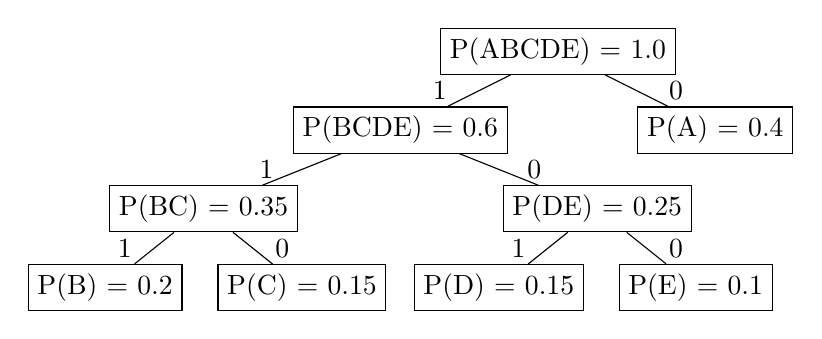
\begin{tikzpicture}[level distance=1cm,
                level 1/.style={sibling distance=4cm},
                level 2/.style={sibling distance=5cm},
                level 3/.style={sibling distance=2.5cm}]
                \node [rectangle, draw]{P(ABCDE) = 1.0}
                    child {node [rectangle, draw]{P(BCDE) = 0.6}
                        child {node [rectangle, draw]{P(BC) = 0.35}
                            child {node [rectangle, draw]{P(B) = 0.2}}
                            child {node [rectangle, draw]{P(C) = 0.15}}}
                        child {node [rectangle, draw]{P(DE) = 0.25}
                            child {node [rectangle, draw]{P(D) = 0.15}}
                            child {node [rectangle, draw]{P(E) = 0.1}}}}
                    child {node [rectangle, draw]{P(A) = 0.4}};
                \node at (1.5, -0.5) {0};
                \node at (-1.5, -0.5) {1};
                \node at (-3.7, -1.5) {1};
                \node at (-0.3, -1.5) {0};
                \node at (-3.5, -2.5) {0};
                \node at (-5.5, -2.5) {1};
                \node at (-0.5, -2.5) {1};
                \node at (1.5, -2.5) {0};
        \end{tikzpicture}
    \end{center}
    The resulting Huffman codes for the symbols are:
    \[
        A = 0, \quad B = 111, \quad C = 110, \quad D = 101, \quad E = 100
    \]
    The average code length is:
    \[
        L = 0.4 \cdot 1 + 0.2 \cdot 3 + 0.15 \cdot 3 + 0.15 \cdot 3 + 0.1 \cdot 3 = 0.4 + 0.6 + 0.45 + 0.45 + 0.3 = 2.2 \text{ bits}
    \]
    The entropy of the source is:
    \[
        H(X) = -\left(0.4 \log_2 0.4 + 0.2 \log_2 0.2 + 0.15 \log_2 0.15 + 0.15 \log_2 0.15 + 0.1 \log_2 0.1\right) \approx 2.17 \text{ bits}
    \]
    $\therefore$ \hl{The average code length of the Huffman code is close to the entropy of the source, indicating that Huffman coding is an}\\ 
    \hspace{0.3cm} \hl{efficient method for compressing data.}\\
\end{egBox}            
$\implies$ The Huffman coding algorithm is optimal for the given symbols and their probabilities, which satisfies Shannon's noiseless \\
\hspace{0.8cm} coding theorem.
\newpage
\textcolor{magenta}{\section{\textbf{Noisy Channels}}}
\subsection{Introduction to Noisy Channels}
In practical communication systems, the received messages may \textcolor{purple}{not match the transmitted messages} due to \textcolor{red}{noise, interference, or other factors}.\\
\vspace{2mm}
There are various sources of noise in communication systems, such as:\\
$\implies$ \uline{\textbf{e.g.}}: Thermal noise, Electromagnetic interference, Cosmic radiation, Physical obstacles, Component degradation and Cross-talk.\\
\vspace{2mm}
To analyze the communication over noisy channels, we can use the \hl{transition probability matrix}, the definition is as follows:
\begin{defBox}{Definition 10.4}{Transition Probability Matrix}
    The \textcolor{red}{transition probability matrix} $P(y|x)$ is a matrix that describes the \textcolor{blue}{probabilities of transitioning from one state $x$ to another state $y$} in a communication system.\\
    $\implies$ The elements of the matrix are defined as:
    \[
        \boxed{\textcolor{teal}{P(y|x) = P(Y=y|X=x) = \begin{bmatrix} 
            P(Y=0|X=0) & P(Y=0|X=1) \\
            P(Y=1|X=0) & P(Y=1|X=1)
        \end{bmatrix}}}
    \]
    \hspace{8mm} where $P(Y=y|X=x)$ is the conditional probability of receiving $y$ given that $x$ was transmitted.
\end{defBox}
\subsection{Channel Modeling}
\uline{\textbf{Binary Symmetric Channel (BSC)}}\\
\begin{defBox}{Definition 10.5}{Binary Symmetric Channel}
    \begin{wrapfigure}[6]{r}{0.2\textwidth}
        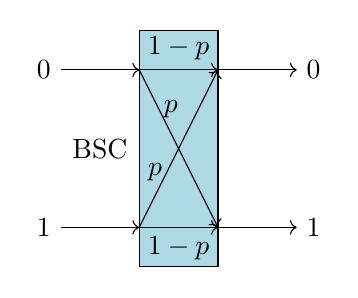
\begin{tikzpicture}
            \draw[fill=lightblue] (1, 0.5) rectangle (2, -2.5);
            \node at (0, 0) [left] {0};
            \draw [->] (0,0) -- (1,0);
            \draw [->] (1,0) -- (2,0) node [midway, above] {$1 - p$};
            \node at (0, -2) [left] {1};
            \draw [->] (0,-2) -- (1,-2);
            \draw [->] (1,-2) -- (2,-2) node [midway, below] {$1 - p$};
            \draw [->] (1,0) -- (2,-2);
            \node at (1.2, -1.3) {$p$};
            \draw [->] (1,-2) -- (2,0);
            \node at (1.4, -0.5) {$p$};
            \draw [->] (2,0) -- (3,0);
            \node at (3, 0) [right] {0};
            \draw [->] (2,-2) -- (3,-2);
            \node at (3, -2) [right] {1};
            \node at (0.5, -1) {BSC};
        \end{tikzpicture}
    \end{wrapfigure}
    The \textcolor{red}{binary symmetric channel (BSC)} is a communication channel that transmits binary symbols (0 or 1) with a certain probability of error.\\
    $\implies$ The transition probability matrix for a BSC is given by:
    \[
        \boxed{\textcolor{teal}{P(y|x) = \begin{bmatrix} 
            1 - p & p \\
            p & 1 - p
        \end{bmatrix}}}
    \]
    where $p$ is the probability of error in the channel.
\end{defBox}

\uline{\textbf{Z-Channel}}\\
\begin{defBox}{Definition 10.6}{Z-Channel}
    \begin{wrapfigure}[6]{r}{0.24\textwidth}
        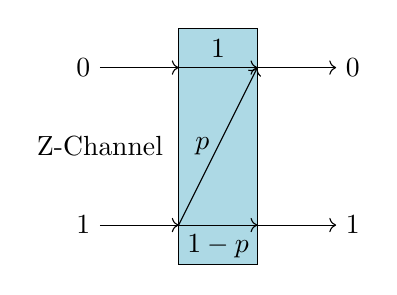
\begin{tikzpicture}
            \draw[fill=lightblue] (1, 0.5) rectangle (2, -2.5);
            \node at (0, 0) [left] {0};
            \draw [->] (0,0) -- (1,0);
            \draw [->] (1,0) -- (2,0) node [midway, above] {$1$};
            \node at (0, -2) [left] {1};
            \draw [->] (0,-2) -- (1,-2);
            \draw [->] (1,-2) -- (2,-2) node [midway, below] {$1 - p$};
            \node at (1.3, -1) {$p$};
            \draw [->] (1,-2) -- (2,0);
            \draw [->] (2,0) -- (3,0);
            \node at (3, 0) [right] {0};
            \draw [->] (2,-2) -- (3,-2);
            \node at (3, -2) [right] {1};
            \node at (0, -1) {Z-Channel};
        \end{tikzpicture}
    \end{wrapfigure}
    The \textcolor{red}{Z-channel} is an binary asymmetric communication channel that \textcolor{blue}{transmits binary symbols (0 or 1) with a certain probability of error, but only for the symbol 1}.\\
    $\implies$ The transition probability matrix for a Z-channel is given by:
    \[
        \boxed{\textcolor{teal}{P(y|x) = \begin{bmatrix} 
            1 & p \\
            0 & 1 - p
        \end{bmatrix}}}
    \]
    where $p$ is the probability of error in the channel.
\end{defBox}
\uline{\textbf{Binary Erasure Channel (BEC)}}\\
\begin{defBox}{Definition 10.7}{Binary Erasure Channel}
    \begin{wrapfigure}[6]{r}{0.22\textwidth}
        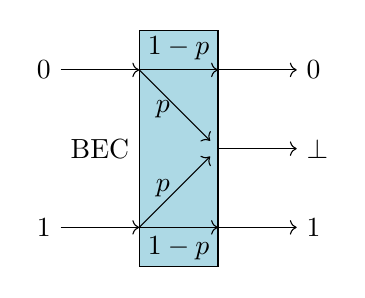
\begin{tikzpicture}
            \draw[fill=lightblue] (1, 0.5) rectangle (2, -2.5);
            \node at (0, 0) [left] {0};
            \draw [->] (0,0) -- (1,0);
            \draw [->] (1,0) -- (2,0) node [midway, above] {$1 - p$};
            \node at (0, -2) [left] {1};
            \draw [->] (0,-2) -- (1,-2);
            \draw [->] (1,-2) -- (2,-2) node [midway, below] {$1 - p$};
            \draw [->] (1,-2) -- (1.9,-1.1);
            \node at (1.3, -1.5) {$p$};
            \node at (1.3, -0.5) {$p$};
            \draw [->] (1,0) -- (1.9,-0.9);
            \draw [->] (2,-1) -- (3,-1);
            \node at (3, -1) [right] {$\perp$};
            \draw [->] (2,0) -- (3,0);
            \node at (3, 0) [right] {0};
            \draw [->] (2,-2) -- (3,-2);
            \node at (3, -2) [right] {1};
            \node at (0.5, -1) {BEC};
        \end{tikzpicture}
    \end{wrapfigure}
    The \textcolor{red}{binary erasure channel (BEC)} is a communication channel that \textcolor{blue}{transmits binary symbols (0 or 1) with a certain probability of erasure}.\\
    $\implies$ The transition probability matrix for a BEC is given by:
    \[
        \boxed{\textcolor{teal}{P(y|x) = \begin{bmatrix} 
            1 - p & 0 & p \\
            0 & 1 - p & p \\
        \end{bmatrix}}}
    \]
    where $p$ is the probability of erasure in the channel.
\end{defBox}

\newpage
\textcolor{magenta}{\section{\textbf{Error Detection and Correction}}}
To combat noise, we need to \textcolor{purple}{detect when errors have occurred} and \textcolor{purple}{correct errors without retransmitting the data}.\\
\vspace{5mm}
\subsection{Repetition Codes}
\begin{defBox}{Definition 10.8}{Repetition Codes}
    \textcolor{red}{Repetition codes} are a simple form of error-correcting codes that \textcolor{blue}{repeat the original message multiple times} to detect and correct errors by using \hl{majority voting}.\\
    $\implies$ The repetition code for a binary message $x$ is defined as:
    \[
        \boxed{\textcolor{teal}{C(x) = x^n = \underbrace{xx\ldots x}_{n \text{ times}}}} \quad \text{where } x \in \{0, 1\} \text{ and } n \text{ is the number of repetitions.}
    \]
\end{defBox}
The repetition code can correct up to $\left\lfloor \frac{n-1}{2} \right\rfloor$ errors in the received message.\\
\vspace{2mm}
Here are the steps to encode and decode a message using repetition codes:
\begin{enumerate}
    \item When a sender transmits a bit, the bit is repeated $n$ times (Note that $n$ is odd).
    \item During transmission, the bits may be flipped due to noise.
    \item The receiver receives the repeated bits and counts the number of 0s and 1s.
    \item The receiver uses majority voting to determine the most likely original bit.
\end{enumerate}
Since the noise only affects each bit independently, the probability of error in the received message is as follows:
\begin{thmBox}{Theorem 10.3}{Probability of Error in Repetition Codes}
    The probability of error in a repetition code with $n$ repetitions is given by:
    \[
        \boxed{\textcolor{red}{P_e = \sum_{k=\left\lfloor \frac{n}{2} \right\rfloor + 1}^{n} \binom{n}{k} p^k (1-p)^{n-k}}} \quad \text{where } p \text{ is the probability of error in each bit.}
    \]
\end{thmBox}
\textcolor{cyan}{As the number of repetitions $n$ increases, the probability of error decreases exponentially}, making repetition codes more reliable.
\begin{egBox}{Example 10.4}{Repetition Codes}
    Consider a binary message $x = 1$ that is transmitted using repetition codes with $n = 5$:
    \[
        C(x) = 11111
    \]
    If the received message is $y = 10111$, we can use majority voting to determine the original bit:
    \begin{itemize}
        \item Count the number of 0s and 1s: $y = 10111$ has 4 ones and 1 zero.
        \item Since the majority is 1, we decode the received message as $x' = 1$.
    \end{itemize}
    Assume the probability of error in each bit is $p = 0.1$. The probability of error in the received message is:
    \begin{align*}
        P_e = \sum_{k=3}^{5} \binom{5}{k} p^k (1-p)^{5-k} = \binom{5}{3} p^3 (1-p)^2 + \binom{5}{4} p^4 (1-p)^1 + \binom{5}{5} p^5 (1-p)^0 &= 10(0.1)^3(0.9)^2 + 5(0.1)^4(0.9)^1 + (0.1)^5 \\
        &= 0.0081 + 0.00045 + 0.00001 = 0.00856
    \end{align*}
    $\therefore$ The probability of error in the received message is approximately 0.00856, which is quite low compared to the original probability of error $p = 0.1$.
\end{egBox}
Even though the repetition codes are simple and effective, they are \hl{extremely inefficient} in terms of bandwidth and storage, as they require $n$ times the amount of data to be transmitted.\\
\newpage
\subsection{Hamming Codes}
\begin{defBox}{Definition 10.9}{Hamming Codes}
    \textcolor{red}{Hamming codes} are a class of error-correcting codes created by Richard Hamming that can \textcolor{blue}{detect and correct single-bit errors in binary messages}.\\
    $\implies$ Hamming codes are based on the \hl{concept of parity bits}, which are added to the original message to create a codeword.
\end{defBox}
\uline{\textbf{Hamming Distances}}\\
\begin{defBox}{Definition 10.10}{Hamming Distance}
    The \textcolor{red}{Hamming distance} between two binary strings of equal length is defined as the \textcolor{blue}{number of positions at which the corresponding bits are different}.\\
    $\implies$ The Hamming distance between two binary strings $x$ and $y$ is denoted as:
    \[
        \boxed{\textcolor{red}{d_H(x, y) = \sum_{i=1}^{n} |x_i - y_i|}} \quad \text{where } n \text{ is the length of the strings.}
    \]
\end{defBox}
The Hamming distance is used to measure the \textcolor{purple}{error-correcting capability} of a code.\\
\vspace{2mm}
The minimum Hamming distance $d_{min}$ of a code is the smallest Hamming distance between any two codewords in the code.\\
$\implies$ The error detection capability $t$ of a code is given by:
\[
    \boxed{\textcolor{teal}{t = d_{min} - 1}} \quad \text{where } t \text{ is the number of errors that can be detected.}
\]
$\implies$ The error-correcting capability $t$ of a code is given by:
\[
    \boxed{\textcolor{teal}{t = \left\lfloor \frac{d_{min} - 1}{2} \right\rfloor}} \quad \text{where } t \text{ is the number of errors that can be corrected.}
\]
\uline{\textbf{(7, 4) Hamming Code}}\\
\begin{defBox}{Definition 10.11}{(7, 4) Hamming Code}
    The \textcolor{red}{(7, 4) Hamming code} is a \textcolor{blue}{linear error-correcting code that encodes 4 bits of data into a 7-bit codeword by adding 3 parity bits}.
\end{defBox}
The syndrome-basedd decoding approach used by the (7, 4) Hamming code is as follows:
\begin{enumerate}
    \item Calculate the parity bits for the received codeword.
    \item Compare the calculated parity bits with the received parity bits.
    \item If there is a mismatch, determine the error position using the syndrome vector.
    \item Flip the bit at the error position to correct the error.
    \item Decode the corrected codeword to retrieve the original message.
\end{enumerate}







\chapter{Quantum Error Correction}
\textcolor{magenta}{\section{\textbf{Introduction to Quantum Error Correction}}}
Quantum error correction is a set of techniques used to protect quantum information from errors due to decoherence and other noise, which is essential for building reliable quantum computers and quantum communication systems.\\
\vspace{2mm}
Quantum error correction codes are designed to detect and correct errors in quantum states without measuring the states directly, which would collapse the quantum state.\\
\vspace{2mm}
The main principles of quantum error correction are:
\begin{itemize}
    \item \textcolor{red}{Redundancy}: Quantum information is encoded in a larger Hilbert space using multiple qubits.
    \item \textcolor{red}{Error Detection}: Errors are detected without measuring the quantum state directly.
    \item \textcolor{red}{Error Correction}: The original quantum state is recovered by applying appropriate correction operations.
    \item \textcolor{red}{Fault Tolerance}: The error correction process is designed to be fault-tolerant, meaning that it can correct errors even if some qubits are affected by noise.
\end{itemize}
To understand quantum error correction, we need to know the concept about quantum error correction codes.\\
\begin{defBox}{Definition 11.1}{Quantum Error Correction Codes}
    \textcolor{red}{Quantum error correction codes} are a set of techniques used to protect quantum information from errors due to decoherence and other noise.\\
    $\implies$ Quantum error correction codes are designed to detect and correct errors in quantum states without measuring the states directly, which would collapse the quantum state.
\end{defBox}
There are 2 examples of quantum error correction codes:
\begin{enumerate}
    \item \textcolor{cyan}{\textbf{Quantum Repetition Code}}.
    \item \textcolor{cyan}{\textbf{Shor 9-Qubit Code}}.
\end{enumerate}



\textcolor{magenta}{\section{\textbf{Quantum Repetition Code}}}
\begin{defBox}{Definition 11.2}{Quantum Repetition Code}
    The \textcolor{red}{quantum repetition code} is a simple quantum error correction code that encodes a single qubit into multiple qubits by repeating the state.\\
    $\implies$ The quantum repetition code can correct errors in the encoded qubit by using majority voting.
\end{defBox}






\textcolor{magenta}{\section{\textbf{Shor 9-Qubit Code}}}
\begin{defBox}{Definition 11.3}{Shor 9-Qubit Code}
    The \textcolor{red}{Shor 9-qubit code} is a quantum error correction code that encodes a single qubit into 9 qubits and can correct arbitrary single-qubit errors.\\
    $\implies$ The Shor 9-qubit code uses a combination of classical error correction techniques and quantum error correction techniques.
\end{defBox}
\section{Encoding Procedure for the Shor 9-Qubit Code}

The Shor code encodes a single logical qubit into 9 physical qubits, protecting against any single-qubit error (bit-flip or phase-flip).

\subsection{Step 1: Express in the $\pm$-basis}
Given an arbitrary qubit
\[
|\psi\rangle = a|0\rangle + b|1\rangle,
\]
rewrite it in the $\{|+\rangle, |-\rangle\}$ basis, where
\[
|+\rangle = \frac{|0\rangle + |1\rangle}{\sqrt{2}}, \quad |-\rangle = \frac{|0\rangle - |1\rangle}{\sqrt{2}}.
\]
Thus,
\[
|\psi\rangle = \alpha|+\rangle + \beta|-\rangle, \quad \text{where} \quad \alpha = \frac{a+b}{\sqrt{2}}, \quad \beta = \frac{a-b}{\sqrt{2}}.
\]

\subsection{Step 2: Phase-Flip Protection (Repetition in $\pm$-basis)}
Encode each $|\pm\rangle$ as a 3-qubit repetition code:
\[
|+\rangle \mapsto |+++\rangle, \qquad |-\rangle \mapsto |---\rangle.
\]
After this step,
\[
|\psi\rangle \mapsto \alpha|+++\rangle + \beta|---\rangle.
\]
This 3-qubit block can correct a single phase-flip ($Z$) error.

% \begin{remark}
% Some conventions map $|0\rangle \mapsto |+++\rangle$ and $|1\rangle \mapsto |---\rangle$ directly. This is just a basis choice and does not affect error correction.
% \end{remark}

\subsection{Step 3: Bit-Flip Protection (Repetition in Computational Basis)}
Now, encode each $|\pm\rangle$ in the computational basis using the 3-qubit bit-flip code:
\[
|+\rangle \mapsto \frac{|000\rangle + |111\rangle}{\sqrt{2}}, \qquad |-\rangle \mapsto \frac{|000\rangle - |111\rangle}{\sqrt{2}}.
\]
The final encoded state is
\[
|\psi_L\rangle = \alpha\left(\frac{|000\rangle + |111\rangle}{\sqrt{2}}\right)^{\otimes 3} + \beta\left(\frac{|000\rangle - |111\rangle}{\sqrt{2}}\right)^{\otimes 3}.
\]
Now, the logical qubit is protected against both bit-flip and phase-flip errors.

\section{Error Detection and Correction Procedure}

The Shor code corrects both bit-flip ($X$) and phase-flip ($Z$) errors by using the structure of the encoding.

\subsection{A. Bit-Flip ($X$) Error Correction}

Each group of 3 qubits (blocks $\{q_1,q_2,q_3\}$, $\{q_4,q_5,q_6\}$, $\{q_7,q_8,q_9\}$) forms a classical repetition code. To detect and correct a single $X$ error in a block:

\begin{enumerate}
    \item Measure the parities $q_1 \oplus q_2$ and $q_2 \oplus q_3$ using ancilla qubits and CNOT gates.
    \item The measurement outcomes identify which qubit (if any) was flipped.
    \item Apply an $X$ gate to correct the error if needed.
\end{enumerate}

\textbf{Parity check circuit for one block:}
% \begin{center}
% \begin{quantikz}[row sep=0.4cm, column sep=0.8cm]
% \lstick{$q_1$}      & \ctrl{3} & \qw      & \qw      & \qw           \\
% \lstick{$q_2$}      & \qw      & \ctrl{2} & \ctrl{3} & \qw           \\
% \lstick{$q_3$}      & \qw      & \qw      & \ctrl{1} & \qw           \\
% \lstick{$\ket{0}$}  & \targ{}  & \qw      & \qw      & \meter{$m_{12}$} \\
% \lstick{$\ket{0}$}  & \qw      & \targ{}  & \qw      & \meter{$m_{23}$} \\
% \lstick{$\ket{0}$}  & \qw      & \qw      & \targ{}  & \meter{}      \\
% \end{quantikz}
% \end{center}

\textbf{Correction rule:}
\begin{itemize}
    \item $m_{12}=m_{23}=1$: flip $q_2$
    \item $m_{12}=1$, $m_{23}=0$: flip $q_1$
    \item $m_{12}=0$, $m_{23}=1$: flip $q_3$
    \item $m_{12}=m_{23}=0$: no correction needed
\end{itemize}

Repeat this procedure for all three blocks. In total, $6$ ancilla qubits and $12$ CNOTs are needed for all blocks.

\subsection{B. Phase-Flip ($Z$) Error Correction}

After correcting bit-flip errors, the three blocks together form a repetition code in the $\pm$-basis, which protects against phase-flip errors.

\begin{enumerate}
    \item Apply Hadamard gates to all 9 qubits (converts $Z$ errors to $X$ errors).
    \item Measure the parity between blocks: e.g., measure parity of blocks $\{1,2,3\}$ and $\{4,5,6\}$, and between $\{4,5,6\}$ and $\{7,8,9\}$, using ancilla qubits and CNOTs.
    \item The measurement outcomes identify which block (if any) has a phase-flip error.
    \item Apply a $Z$ gate to correct the error in the identified block.
    \item Apply Hadamard gates again to return to the computational basis.
\end{enumerate}

\textbf{Syndrome extraction circuit:}

\begin{center}
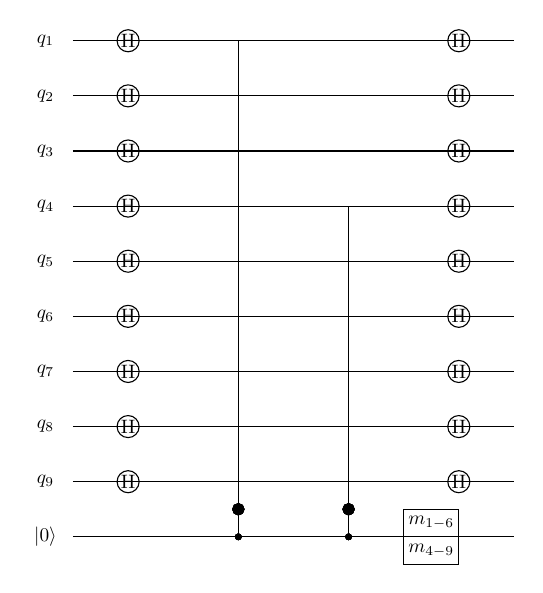
\begin{tikzpicture}[scale=0.7, every node/.style={scale=0.7}]
% Qubit lines
\foreach \y in {0,...,8} {
    \draw (0,-\y) -- (8,-\y);
    \node at (-0.5,-\y) {$q_{\the\numexpr\y+1\relax}$};
}
% Ancilla line
\draw (0,-9) -- (8,-9);
\node at (-0.5,-9) {$\ket{0}$};

% Hadamard gates
\foreach \y in {0,...,8} {
    \draw (1,-\y) circle (0.2) node {H};
}

% CNOT gates for parity checks
% First parity check (q1-q6)
\foreach \y in {0,...,5} {
    \draw (3,-\y) -- (3,-8.5);
    \filldraw (3,-8.5) circle (0.1);
    \draw (3,-9) -- (3,-8.5);
    \filldraw (3,-9) circle (0.05);
}

% Second parity check (q4-q9)
\foreach \y in {3,...,8} {
    \draw (5,-\y) -- (5,-8.5);
    \filldraw (5,-8.5) circle (0.1);
    \draw (5,-9) -- (5,-8.5);
    \filldraw (5,-9) circle (0.05);
}

% Final Hadamards
\foreach \y in {0,...,8} {
    \draw (7,-\y) circle (0.2) node {H};
}

% Measurements
\draw (6,-9) rectangle (7,-8.5) node[pos=0.5] {$m_{1-6}$};
\draw (6,-9.5) rectangle (7,-9) node[pos=0.5] {$m_{4-9}$};
\end{tikzpicture}
\end{center}

\textbf{Summary:}
\begin{itemize}
    \item The Shor code corrects any single-qubit error by first correcting bit-flip errors within each block, then correcting phase-flip errors across blocks.
    \item Error syndromes are extracted using ancilla qubits and CNOTs, and corrections are applied accordingly.
\end{itemize}


\end{document}